\documentclass[11pt,a4paper]{report}

\usepackage[left=2cm,right=2cm,top=2cm,bottom=2cm]{geometry}
\usepackage{hyperref}
\usepackage{pythonhighlight}
\usepackage{enumitem} 
\usepackage[yyyymmdd,hhmmss]{datetime}
\usepackage{amsmath}
\usepackage[utf8]{inputenc}
\usepackage{color}
\usepackage{xcolor}
\usepackage{graphicx}
\usepackage{subcaption}
\usepackage{float}
\usepackage{booktabs}
\usepackage[square,sort,comma,numbers]{natbib}
\usepackage[linesnumbered,lined,ruled]{algorithm2e}
\usepackage{subfiles}
\usepackage{imakeidx}
\makeindex

\hypersetup{
    colorlinks = true,
    linkcolor  = blue,
    filecolor  = magenta,      
    urlcolor   = magenta
}
\renewcommand{\labelitemii}{$\star$}
\SetEndCharOfAlgoLine{}
\SetAlFnt{\footnotesize\ttfamily}


\begin{document}
\title{Study on Quantitative finance}
\author{Chi Thanh Nguyen}
\date{\today \@ \currenttime}
\maketitle

\tableofcontents


\chapter{Introduction}
This is my study note on the subject of Quantitative Finance based mainly on the book \cite{pw_iqf2ed_2007}. I do hope that in the very near future I can successfully move to the finance sector and work as a Quantitative Investment Researcher. 


\appendix 
\chapter{Brief on quantitative finance}
This chapter is a very brief introduction to quantitative finance, more precisely, a collection of definitions concerning the financial markets which relate to the quantitative finance. The content of this chapter is based heavily on \cite{pw_iqf2ed_2007, ch_ofd9ed_2015}.


\section{Products and markets}
\subsection{Equities}
The most basic of financial instruments is the  \textbf{equity}\index{equity}, \textbf{stock}\index{stock} or \textbf{share}\index{share}. This is the ownership of a small piece of a company. Shares can be bought and sold freely on a regulated stock exchanges and capital can be raised efficiently. The behavior of the stock prices is far from being predictable because the prices have a large element of randomness. Therefore, the modeling must be done in a probabilistic sense. 

The value in holding stocks comes from the \textbf{dividends}\index{dividends} and any growth in the stock's value. Dividends are lump sum payments, paid out every quarter or every six months, to the holder of stock. The amount of the dividend varies depending on the profitability of the company. When the stock is bought, it either comes with its entitlement to the next dividends (\textbf{cum}\index{cum-dividend}) or not (\textbf{ex}\index{ex-dividend}). 

A stock is normally announced in a \textbf{stock-split}\index{stock-split}, e.g. a company with a stock price of \$90 announces a three-for-one split which simply means that instead of holding one stock valued at \$90, one holds three valued at \$30 each.
 
 
\subsection{Commodities}
Commodities are usually raw products such as precious metals, oil, etc. The prices of these products are unpredictable but often show seasonal effects. Commodities are usually traded by people who have no need of the raw material. Most trading is done on the futures market, making deals to buy or sell the commodity at some time in the future. The deal is then closed out before the commodity is due to be delivered. Futures contracts are discussed later.


\subsection{Currencies}
Countries in the world use different currencies, the rate at which one currency can be exchanged for another is the \textbf{exchange rate}\index{exchange rate}. This is the world of \textbf{foreign exchange}\index{foreign exchange}, or \textbf{Forex}\index{Forex} or \textbf{FX}\index{FX} for short. Whatever the exchange rates from one currency to another, there must be consistency throughout; otherwise it is possible to make \textbf{arbitrage profits}\index{arbitrage profits} by exploiting the mispricing.


\subsection{Indices}
For measuring how the stock market/economy is doing as whole, the stock market \textbf{indices}\index{indices} have been developed. A typical \textbf{index}\index{index} is made up from the weighted sum of a selection or \textbf{basket}\index{basket} of representative stocks. The selection may be designed to represent the whole market, such as the S\&P500 in the US or the FTSE100 in the UK, or a very special part of a market


\subsection{The time value of money}
The most fundamental concept in finance is the \textbf{time value of money}\index{time value of money}. \$100 today is worth more than \$100 in a year because of all the things we can do with \$100 over the year. You can lend the money to someone who can invest it in various risky ways (e.g. banks) and give you back the money with a little bit extra, the \textbf{interest}\index{interest}.

Let's denote the interest rates by $r$ and assume, for the moment, that $r$ are constant. Two most basic types of interest are simple and \textbf{compound}\index{compound}. Simple interest is when the interest is based only on the initial amount, whereas compound interest is when the interest has interest also. In reality, compound interest is the only case of relevance. Compound interest has two forms, \textbf{discretely compounded}\index{discretely compounded} and \textbf{continuously compounded}\index{continuously compounded}. The difference of these two types are illustrated below. 

\begin{center}
\begin{footnotesize}
\fbox{
\begin{minipage}{0.90\textwidth}
Suppose we invest \$100 in a bank at a discrete interest rate of $r$ paid \textit{once per annum}. After one year, the money becomes:
\begin{equation}
    100 \times \left( 1 + r \right)
\end{equation} 
and after $n$ years, we have:
\begin{equation}
    100 \times \left( 1 + r \right)^n
\end{equation}

Now, suppose there are $m$ interest payments at a rate of $r/m$ \textit{per annum}. After one year, the money in the bank is:
\begin{equation}
    100 \times \left( 1 + \frac{r}{m} \right)^m
\end{equation} 
Imagine that the interest payments come at increasingly frequent intervals, but at an increasingly smaller interest rate, this will lead to a rate of interest that is paid continuously. After one year, the money in the bank is:
\begin{equation}
    \lim_{m \to \infty}{100 \times \left( 1 + \frac{r}{m} \right)^m} \sim 100 \times e^r
\end{equation} 
And similarly, after $t$ years, we will have the amount:
\begin{equation}
    100 \times \left( 1 + \frac{r}{m} \right)^{mt} \sim 100 \times e^{rt}
    \label{cont_comp}
\end{equation} 

Equation \ref{cont_comp} can be derived via a differential equation. Suppose we have an amount $M(t)$ in the bank at time $t$. A short while later, time $t + dt$, the amount will have increased by:
\begin{equation}
    M(t+dt) - M(t) \approx \frac{dM}{dt}dt + \cdots 
\end{equation} 
where the rhs is a Taylor polynomial approximation. On the other hand, the interest we receive must be proportional to the amount we have $M$, the interest rate $r$ and the time step $dt$. Therefore:
\begin{equation}
    \frac{dM}{dt}dt = r \times M(t) dt \to \frac{dM}{dt} = r \times M(t)
\end{equation} 
This is the ordinary differential equation with the solution:
\begin{equation}
    M(t) = M(0) \times e^{rt}
\end{equation} 

The interest rate presented above is an important factor to relate the \textbf{present value}\index{present value}, $M(t)$, with the \textbf{future value}\index{future value}, $M(T)$, of the money as follows:
\begin{equation}
    M(t) = M(T) \times e^{-r(T-t)}
\end{equation} 
\end{minipage}
}
\end{footnotesize}
\end{center}


\subsection{Fixed-income securities}
A \textbf{fixed-income security}\index{fixed-income security} is an investment that provides a return in the form of \textbf{fixed periodic interest payments}\index{fixed periodic interest payment} and the eventual return of \textbf{principal at maturity}\index{principal at maturity}. Unlike \textbf{variable-income securities}\index{variable-income security}, where payments change based on some underlying measure — such as \textbf{short-term interest rates} or \textbf{floating interest rates}\index{floating interest payment} — the payments of a fixed-income security are known in advance. \textbf{Interest rate swaps}\index{interest rate swaps} are an exchange of a fixed rate of interest for a floating rate of interest.

There are various types of fixed income securities, such as:

\begin{itemize}
    \setlength\itemsep{0em}
    \item Bonds (both corporate and government) - the most common form of fixed-income securities;
    \item Treasury Bills;
    \item Money market instruments;
    \item Asset-backed securities.
\end{itemize}

The \textbf{index-linked bond}\index{index-linked bond} has been in the UK since 1981 and have provided a successful way to ensuring that income is not eroded by inflation (an inflation-proof bond). In the UK inflation is measured by the \href{https://www.investopedia.com/terms/r/rpi.asp}{\textbf{Retail Price Index (RPI)}}\index{Retail Price Index}; in the US the inflation index is the \href{https://www.investopedia.com/terms/c/consumerpriceindex.asp}{\textbf{Consumer Price Index (CPI)}}\index{Consumer Price Index}. The dynamics of the relationship between inflation and short-term interest rates is particularly interesting; the level of interest rates will affect the rate of inflation, but also interest rates are often used by central banks as a tool for keeping inflation down.


\subsection{Forwards and futures}
A \href{https://en.wikipedia.org/wiki/Forward_contract}{\textbf{forward contract}}\index{forward contract} is a private agreement between two parties giving the buyer an obligation to purchase an asset (and the seller an obligation to sell an asset) at a specified price (\textbf{the delivery price}\index{delivery price}) at a specified time (\textbf{the delivery date}\index{delivery date}) in the future. No money changes hands until the delivery date or \textbf{maturity}\index{maturity} of the contract. The asset could be a stock, a commodity or a currency. The \href{https://investinganswers.com/dictionary/f/forward-contract}{forward contract} has a value of zero initially. As we approach maturity, the value of the contract will change from initially zero to the difference between the underlying asset and the delivery price, at maturity.

A \href{https://en.wikipedia.org/wiki/Futures_contract}{\textbf{futures contract}}\index{futures contract} is very similar to a forward contract. \href{https://investinganswers.com/dictionary/f/futures-contract}{Futures contracts} are usually traded through an exchange, which standardizes the terms of the contracts - standardization means the same thing to everyone in the market. The profit or loss from the futures position is calculated every day and the change in this value is paid from one party to the other. Thus with futures contracts there is a gradual payment of funds from initiation until maturity. Because the change in value is settled on a daily basis, the value of a futures contract at any time during its life is zero. The different between the forward contracts and the future contracts can be found \href{https://en.wikipedia.org/wiki/Futures_contract}{here} or \href{https://www.investopedia.com/ask/answers/06/forwardsandfutures.asp}{here}. A series of brief lessons for forward and future contracts can be found \href{https://financetrain.com/series/futures-forwards/}{here}.

There are two kinds of forward- and future-contract participants: hedgers and speculators. Hedgers do not usually seek a profit but rather seek to stabilize the revenues or costs of their business operations; therefore hedging is avoidance of risk. Their gains or losses are usually offset to some degree by a corresponding loss or gain in the market for the underlying asset. Speculators are usually not interested in taking possession of the underlying assets. They essentially place bets on which way prices will go. 

Forward contracts tend to attract more hedgers than speculators. Speculators are often blamed for big price swings, but they also provide a lot of liquidity to the futures market. Look at section 1.9.1 in \cite{pw_iqf2ed_2007} for a hedged portfolio of asset and forward and the \textbf{no-arbitrage}\index{no-arbitrage} principle.

\begin{center}
\begin{footnotesize}
\fbox{
\begin{minipage}{0.90\textwidth}
Consider a forward contract that obliges us to hand over an amount \$$F$ at time $T$ to receive the underlying asset. Today's date is $t$ and the price of the asset is currently \$$S(t)$ - the \textbf{spot price}\index{spot price}. At maturity, we will hand over the amount \$$F$ and receive the asset then worth \$$S(T)$.

Assume that we simultaneously sell the asset when we enter into the forward contract - \textbf{going short}\index{going short} when we sell something we don't own. Now, we have an amount of $S(t)$ in cash due to the sale of the asset, a forward contract and a short asset position. Our net position now is zero. Then, we put the cash in the bank to receive interest. 
  
At maturity, we hand over the amount $F$ and receive the asset of $S(T)$ - this cancels our short asset position. We are also left with \textit{guaranteed} -$F$ in cash and the bank account with the initial investment of $S(t)$ with added interest. Our net position at maturity is then:
\begin{equation}
    S(t) \times e^{r(T-t)}-F
\end{equation}

Because we began with a portfolio worth zero and we end up with a predictable amount, that amount should also be zero (following the no-arbitrage principle). We can conclude that:
\begin{equation}
    F = S(t) \times e^{r(T-t)}
\end{equation}

This is the relationship between the spot price and the forward price. It is a linear relationship, the forward price is proportional to the spot price. If this relationship is violated then there will be an arbitrage opportunity. The standard economic argument then says that investors will act quickly to exploit the opportunity, and in the process prices will adjust to eliminate it.
\end{minipage}
}
\end{footnotesize}
\end{center}

Futures are usually traded publicly through an exchange which means they are very liquid
instruments and have lots of rules and regulations surrounding them. Here are a few
concepts related futures contracts.
\begin{itemize}
    \setlength\itemsep{0em}
    \item Available assets: a futures contract will specify the asset which is being invested in, the contract also specifies how many of each asset must be delivered, and the quantity will depend on the market. As an asset, a natural \href{https://en.wikipedia.org/wiki/Commodity}{\textbf{commodity}}\index{commodity} is particularly interesting because of non-uniformity in the type and quality of the asset to be delivered.
    \item Delivery and settlement: the futures contract will specify when the asset is to be delivered and settlement is the act of consummating the contract. The contract can be settled in \href{https://financetrain.com/settlement-of-futures-contracts/}{three ways}: (1) \textbf{closeout}\index{closeout}, (2) \textbf{physical delivery}\index{physical delivery} and (3) \textbf{cash settlement}\index{cash settlement}. Most futures contracts are closed out before delivery, with the trader taking the opposite position before maturity.
    \item Margin: changes in the value of futures contracts are settled each day - \textbf{marking to market}\index{marking to market}. To reduce the likelihood of one party defaulting, being unable or unwilling to pay up, the exchanges insist on traders depositing a sum of money to cover changes in the value of their positions. This money is deposited in a \textbf{margin account}\index{margin account}. Margin comes in two forms, the \textbf{initial margin}\index{initial margin} and the \textbf{maintenance margin}\index{maintenance margin}. The initial margin is the amount deposited at the initiation of the contract. The total amount held as margin must stay above a prescribed maintenance margin. If it ever falls below this level then more money (or equivalent in bonds, stocks, etc.) must be deposited. 
    \item Commodity futures: futures on commodities don't necessarily obey the no-arbitrage law that led to the asset/future price relationship because of the messy topic of storage. The holder of the futures contract must compensate the holder of the commodity for his storage costs. This can be expressed in percentage terms by an adjustment $s$ to the risk-free rate of interest. On the other hands, most people actually holding the commodity are benefiting from it in some way. And the benefit from holding the commodity is commonly measured in terms of the convenience yield $c$:
\begin{equation}
    F = S(t) \times e^{(r+s-c)(T-t)}
\end{equation}
Depending on the storage cost and the convenience yield, the price varies. When 
\begin{equation}
    F < S(t) \times e^{r(T-t)}
\end{equation}
the market is said to be \textbf{backwardation}\index{backwardation}; when 
\begin{equation}
    F > S(t) \times e^{r(T-t)}
\end{equation}
the market is said to be \textbf{contango}\index{contango}.
    \item FX futures: there are no problems associated with storage when the asset is a currency, we only need to modify the no-arbitrage result to allow for interest received on the foreign currency $r_f$. Then we have:
    \begin{equation}
    F = S(t) \times e^{(r-r_f)(T-t)}
\end{equation}
    \item Index futures: futures contracts on stock indices are settled in cash. Again, there are no storage problems, but now we have dividends, which play a role similar to that of a foreign interest rate on FX futures, to contend by the dividend yield $q$. 
\begin{equation}
    F = S(t) \times e^{(r-q)(T-t)}
\end{equation}
\end{itemize}

Here are the summary of a few loose definitions for the important financial terminologies that have been presented above. 
\begin{itemize}
    \setlength\itemsep{0em}
    \item \textbf{Premium}\index{premium}: the amount paid for the contract initially.
    \item \textbf{Underlying (asset)}\index{underlying asset} the financial instrument on which the option value depends denoted by $S$. The option payoff is defined as some function of the underlying asset at expiry.
    \item \textbf{Strike (price)} or \textbf{exercise price}: the amount for which the underlying can be bought (call) or sold (put) denoted by $E$. This definition only really applies to the simple calls and puts.
    \item \textbf{Expiration (date)} or \textbf{expiry (date)}: date on which the option can be exercised or date on which the option ceases to exist or give the holder any rights denoted by $T$.
    \item \textbf{Intrinsic value}\index{intrinsic value}: the payoff that would be received if the underlying is at its current level when the option expires.
    \item \textbf{Time value}\index{time value}: any value that the option has above its intrinsic value since the option value is generally different from the intrinsic value.
    \item \textbf{In the money}\index{in the money}: an option with positive intrinsic value. A call option when the asset price is above the strike, a put option when the asset price is below the strike.
    \item \textbf{Out of the money}\index{out of the money}: an option with no intrinsic value, only time value. A call option when the asset price is below the strike, a put option when the asset price is above the strike.
    \item \textbf{At the money}\index{at the money}: a call or put with a strike that is close to the current asset level.
    \item \textbf{Long position}\index{long position}: a positive amount of a quantity, or a positive exposure to a quantity.
    \item \textbf{Short position}\index{short position}: a negative amount of a quantity, or a negative exposure to a quantity. Many assets can be sold short, with some constraints on the length of time before they must be bought back. More explanation for the long and short position can be found \href{http://positron-investments.com/en/technical-analysis-basics/long-versus-short-selling/}{here}.
\end{itemize}


\section{Derivatives}
\subsection{Options}
In the future or forward contracts, the holder is obliged to trade at the maturity of the contract. The \textbf{option}\index{option} gives the holder the \textit{right} to trade in the future at a previously agreed price but takes away the obligation, e.g. if the stock falls, we don't have to buy it after all. A \textbf{call option}\index{call option} is the right to buy a particular asset for an agreed amount (the \textbf{exercise price}\index{exercise price} or \textbf{strike price}\index{strike price}) at a specified time in the future (the \textbf{expiry}\index{expiry} or \textbf{expiration date}\index{expiration date}). The stock on which the option is based is known as the \textbf{underlying asset}\index{underlying asset}. We would exercise the option at expiry if the stock is above the strike and not if it is below. If we use $S$ to mean the stock price and $E$ the strike then at expiry the option is worth:
\begin{equation}
    \max(S - E, 0)
\end{equation}
This function of the underlying asset is called the \textbf{payoff function}\index{payoff function}.

A \textbf{put option}\index{put option} is the right to sell a particular asset for an agreed amount at a specified time in the future. The holder of a put option wants the stock price to fall so that he can sell the asset for more than it is worth. The payoff function for a put option is:
\begin{equation}
    \max(E - S, 0)
\end{equation}
And now the option is only exercised if the stock falls below the strike price.

Calls and puts have a non-linear dependence on the underlying asset. The randomness in the underlying asset and the curvature of the option value with respect to the asset are intimately related. Other terms used to describe contracts with some dependence on a more fundamental asset are \textbf{derivatives}\index{derivatives} or \textbf{contingent claims}\index{contingent claim}.

An option's value at expiry is normally visualized in a \href{http://positron-investments.com/en/options-basics/payoff-diagrams/}{\textbf{payoff diagram}}\index{payoff diagram} in which the value of an option at expiry is a function of the underlying, or in a \textbf{profit diagram}\index{profit diagram} in which the payoff subtracted by the premium originally paid for the call option is a function of the underlying. More explanation on the loss/profit diagram can be found \href{https://www.optiontradingtips.com/options101/payoff-diagrams.html}{here}.

The \href{http://positron-investments.com/en/options-basics/option-buyer-vs-option-writer/}{\textbf{writer}}\index{writer} of an option is the person who promises to deliver the underlying asset, if the option is a call, or buy it, if the option is a put. The writer is the person who receives the premium. Writing options is very risky. The downside of buying an option is just the initial premium, the upside may be unlimited. The upside of writing an option is limited, but the downside could be huge. To cover the risk of default in the event of an unfavorable outcome, the \textbf{clearing houses}\index{clearing houses} that register and settle options insist on the deposit of a margin by the writers of options.

Most of the simpler options contracts are bought and sold through \textbf{exchanges}\index{exchange}. These exchanges make it simpler and more efficient to match buyers with sellers. Part of this simplification involves the conventions about features of the contracts. Having standardized contracts traded through an exchange promotes liquidity of the instruments. Some options are an agreement between two parties, often brought together by an intermediary. These agreements can be very flexible and the contract details do not need to satisfy any conventions. Such contracts are known as \textbf{over the counter}\index{over the counter} or \textbf{OTC}\index{OTC} contracts.


\subsection{The value of the option}
The \textit{fair value} of the option contracts $V$ depends on the underlying asset price $S$ and time $t$, $V(S,t)$. At the expiry date $t = T$, the function $V$ is the payoff function, e.g. for the call option:
\begin{equation}
    V(S,T) = \max(S - E, 0)
\end{equation}    

Factors influencing the derivative prices consists of \textbf{variables}\index{variables} (e.g. the value of the underlying asset $S$ and the time to expiry $t$) and \textbf{parameters}\index{parameters} (e.g. the interest rate and the strike price). There is one important parameter which has a major impact on the option value. That parameter is the \textbf{volatility}\index{volatility} which is a measure of the amount of fluctuation in the asset price, a measure of the randomness. Volatility is a particularly interesting parameter because it is so hard to estimate since it never stays constant and is unpredictable.


\subsection{Speculation and gearing}
If you buy a far out-of-the-money option it may not cost very much, especially if there is not very long until expiry. If the option expires worthless, then you also have not lost very much. However, if there is a dramatic move in the underlying, so that the option expires in the money, you may make a large profit relative to the amount of the investment. This is an example of \textbf{gearing}\index{gearing} or \textbf{leverage}\index{leverage}. The out-of-the-money option has a high gearing, a possible high payoff for a small investment. The downside of this \href{https://en.wikipedia.org/wiki/Leverage_(finance)}{leverage} is that the call option is more likely than not to expire completely worthless and you will lose all of your investment. Further reading about gearing and leverage can be found in \href{https://www.investopedia.com/terms/l/leverageratio.asp}{here}, \href{https://www.investopedia.com/terms/g/gearingratio.asp}{here} and \href{https://specialties.bayt.com/en/specialties/q/146664/what-is-the-difference-between-leverage-ratio-and-gearing-ratio/}{here}

Due to the unpredictable adverse price movements in an asset, the writer of the option normally buy other contracts to offset his risk. This offsetting of risk by buying other related contracts is called \textbf{hedging}\index{hedging}. \href{https://en.wikipedia.org/wiki/Hedge_(finance)}{Hedging} is the practice of taking a position in one market to offset and balance against the risk adopted by assuming a position in a contrary or opposing market or investment. Further reading about hedging can be found in \href{https://www.investopedia.com/terms/h/hedge.asp}{here} and \href{https://www.investopedia.com/trading/hedging-beginners-guide/}{here}.


\subsection{Option strategies}
\subsubsection{Single-option}
Calls and puts are the two simplest forms of option, they are often referred to as \textbf{vanilla}\index{vanilla}. Increasingly important are the \textbf{binary}\index{binary option} or \textbf{digital options}\index{digital option}. Binary options have an expiry date and/or time. At the time of expiry, the price of the underlying asset must be on the correct side of the strike price (based on the trade taken) for the trader to make a profit. Further explanations on the binary options can be found \href{https://www.investopedia.com/terms/b/binary-option.asp}{here}.

Three other popular options in practice are:
\begin{itemize}
    \setlength\itemsep{0em}
    \item \textbf{American options}\index{American option} which can be exercised at any time up to the maturity;
    \item \textbf{European options}\index{European option} which can be exercised only on the expiration date itself; and,
    \item \textbf{Bermudan options}\index{Bermudan option} which allow exercise on specified dates or in specified periods.
\end{itemize} 


\subsubsection{Put-Call parity}
Imagine that today at $t$ you buy one European call option with a strike of $E$ and an expiry of $T$ and that you write a European put option with the same strike and expiry, you now have a pair of long-call and short-put. The payoff for the portfolio of the two options is the sum of the individual payoffs:
\begin{equation}
    \max(S(T) - E, 0) - \max(E - S(T), 0) = S(T) - E
\end{equation}  
where $S(T)$ is the value of the underlying asset at time $T$, today it cost you $S(t)$. 

The cash-flow of the portfolio is independent of the future behaviour of the stock and is modelled as:
\begin{equation}
    C - P = S - Ee^{-r(T-t)}
\end{equation}  
where $C$ and $P$ are today's values of the call and the put respectively. This relationship holds at any time up to expiry and is known as the \textbf{put-call parity}\index{put-call parity}. If this relationship did not hold then there would be riskless arbitrage opportunities.
 

\subsubsection{Multiple-option}
In a portfolio, normally several different options are combined to maximize the profit or minimize the risk. There are numerous combinations in practice, a few simple one can be listed as:
\begin{itemize}
    \setlength\itemsep{0em}
    \item \href{https://www.investopedia.com/terms/s/spread.asp}{Spread}
    \item \href{https://www.investopedia.com/terms/b/bullspread.asp}{Bull spread}
    \item \href{https://www.investopedia.com/terms/b/bearspread.asp}{Bear spread}
    \item \href{https://www.investopedia.com/terms/c/condorspread.asp}{Condor spread}
    \item \href{https://www.investopedia.com/terms/c/calendarspread.asp}{Calendar spread}
    \item \href{https://www.investopedia.com/terms/c/creditspread.asp}{Credit spread}
    \item \href{https://www.investopedia.com/terms/d/debitspread.asp}{Debit spread}
    \item \href{https://brilliant.org/wiki/straddle-strangle/}{Straddle and Strangle} and \href{https://www.investopedia.com/ask/answers/05/052805.asp}{their differences}
    \item Risk reversal 
\end{itemize}


\subsubsection{Miscellaneous}
\begin{itemize}
    \setlength\itemsep{0em}
    \item \textbf{Warrants}\index{warrant}: a contract that is very similar to an option is a warrant.Warrants are call options issued by a company on its own equity. The main differences between traded options and warrants are the timescales involved, warrants usually have a longer lifespan, and on exercise the company issues new stock to the warrant holder. On exercise, the holder of a traded option receives stock that has already been issued.
    \item \textbf{Convertible bonds}\index{convertible bond}: convertible bonds (or \textbf{CBs}) have features of both bonds and warrants. They pay a stream of coupons with a final repayment of principal at maturity, but they can be converted into the underlying stock before expiry. Because the CB can be converted into the asset, its value has to be at least the value of the asset. This makes CBs similar to American options
    \item \textbf{Over-the-Counter (OTC)}\index{over-the-counter, OTC} options: Not all options are traded on an exchange. Some, known as over the counter or OTC options, are sold privately from one counter-party to another.
\end{itemize}



\section{The binomial model}
\label{sec:intro_binomial_model}
\subsection{Introduction}
The binomial model is the simplest model for asset prices that can be used for pricing derivatives and to explain a couple of very important financial concepts. The original binomial concept is due to Cox et al. \cite{cox_optionpricing_1979}. More details description of the model can be found in \cite{pw_poqf2ed_2006, pw_iqf2ed_2007, ch_ofd9ed_2015}. Hull \cite{ch_ofd9ed_2015} also describes its use in the fixed-income world. Mathematical treatment of the binomial model is briefly presented in Section \ref{sec:binomial_tree}. This section only summaries the main idea of the binomial model based on the illustration in Chapter 3 of \cite{pw_iqf2ed_2007}.

\begin{center}
\begin{footnotesize}
\fbox{
\begin{minipage}{0.90\textwidth}
The model is used for the behavior of an equity, e.g. a stock and to illustrate how to value options. The starting point of the model includes:
\begin{itemize}
    \setlength\itemsep{0em}
    \item We will have a stock currently worth \$100.
    \item The stock can either rise or fall by a known amount at a known probability between today and tomorrow; a rise to \$101 with a probability of 0.6 and a fall to \$99 with a probability of 0.4. 
    \item Interest rates are zero.
\end{itemize}

We have the call option on the stock with a strike of \$100 and expires tomorrow. The question is what the option is worth today ? Sadly, not \textbf{0.6} as you may calculate with the rise/fall amounts and the corresponding probability, but \textbf{0.5}. 

To understand the option value of 0.5, we must construct a portfolio consisting of one option and short $\frac{1}{2}$ of the underlying stock. By doing so, the portfolio takes the value of $-\frac{99}{2}$ regardless of whether the stock rises or falls. This portfolio is a perfectly \textbf{risk-free portfolio}\index{risk-free portfolio}. As the portfolio is worth $-\frac{99}{2}$ tomorrow and interest rates are zero, it must also be wroth $-\frac{99}{2}$ today. This is an example of \textbf{no arbitrage}\index{no arbitrage}. 

In the above example, the value of an option does not depend on the probability of the stock rising or falling. This is equivalent to saying that the stock growth rate is irrelevant for \href{https://www.investopedia.com/terms/o/optionpricingtheory.asp}{option pricing}. This is because we have \textbf{hedged} \textit{the option with the stock} hence we do not care whether the stock rises or falls.

The quantity of stock that much be sold for hedging is $\frac{1}{2}$. This is called as \textbf{Delta-hedging}\index{Delta-hedging}, $\Delta$, which means choosing a proportion such that the portfolio value does not depend on the direction of the stock. In general:
\begin{equation}
    \Delta = \frac{\text{range of option payoffs}}{\text{range of stock prices}} = \frac{1-0}{101-99} = \frac{1}{2}
\end{equation}
which actually comes from the equality:
\begin{equation}
    1 - \Delta \times 101 = 0 - \Delta \times 99
\end{equation}
$\Delta$ can represent the sensitivity of the option to changes in the stock.

How does the option value change if the interest rate is non-zero? We still delta-hedge as before to construct a risk-free portfolio, then we use exactly the same delta to present value that back in time by multiplying by a discount factor. 

Assume that $r = 0.1$ then the discount factor for going back one day is:
\begin{equation}
    \frac{1}{1+0.1/252} = 0.9996
\end{equation}

The portfolio value today must be the \textit{present value} of the portfolio value tomorrow:
\begin{equation}
    ? - 0.5 \times 100 = 0 - 0.5 \times 99 \times 0.9996
\end{equation}
so that $? = 0.51963$.
\end{minipage}
}
\end{footnotesize}
\end{center}

The \textbf{theoretical price}\index{theoretical price} derived above should be identical to the \textbf{market price}\index{market price} otherwise there is risk-free money to be made. If the option costs less than 0.5 simply buy it and hedge to make a profit. If it is worth more than 0.5 in the market then sell it and hedge, and make a guaranteed profit. In reality, it is possible for arbitrage opportunities to exist, and to exist for a long time. The market also really need there to be some practical mechanism for arbitrage to be `removed'. Supply and demand should act to make the option price converge to the 0.5.


\subsection{Risk-neutrality}
In the \textbf{real world}\index{real world}, statistical skills have been used to estimate the future possible stock prices (99 and 101) and the probabilities of reaching them (0.4 and 0.6). Some properties of the real world can be listed as (1) we know about delta hedging and risk elimination; (2) we are sensitive to risk and expect greater return for taking risk; and (3) only the two stock prices matter for option pricing, not the probabilities.

People often refer to the \textbf{\href{https://www.investopedia.com/terms/r/riskneutral.asp}{risk-neutral} world}\index{risk-neutral world} in which people don't care about risk. The risk-neutral world has the following characteristics (1) we don't care about risk, and don't expect any extra return for taking unnecessary risk; (2) we don't ever need statistics for estimating probabilities of events happening; and (3) we believe that everything is priced using \textbf{simple expectations}.

\begin{center}
\begin{footnotesize}
\fbox{
\begin{minipage}{0.90\textwidth}
Imagine that we are in the risk-neutral world and:
\begin{itemize}
    \setlength\itemsep{0em}
    \item we have a stock currently worth \$100;
    \item the stock can either rise to \$101 or fall to \$99. 
\end{itemize}

Using simple expectation and the symmetry of rising/falling, the \textbf{risk-neutral probability}\index{risk-neutral probability} $p'$ can be calculated from:
\begin{equation}
    p' \times 101 + (1-p') \times 99 = 100
\end{equation}
hence $p' = 0.5$. Please note that $p'$ is only a mathematical term, it is not real since it is derived based on a fundamentally wrong assumption that simple expectations are used for pricing, hence no allowance has been made for risk.

If we just continue to value the call option based on $p'$ and the simple expectation we have:
\begin{equation}
    ? = p' \times 1 + (1-p') \times 0 = 0.5
\end{equation}
This is called the \textbf{risk-neutral expectation}\index{risk-neutral expectation} and it is correct. So actually two times of wrongly-using `simple expectation' cancel each other out. 

When interest rates are non-zero we must perform exactly the same operations but whenever we equate values at different times we must allow for present valuing. For example, with $r = 0.1$, we calculate the risk-neutral probability from:
\begin{equation}
    \frac{1}{1+0.1/252} \left( p' \times 101 + (1-p') \times 99 \right) = 100
\end{equation}
in which the first term is the discount factor as in the previous example and equal 0.9996; so $p' = 0.51984$.

The expected option payoff is now:
\begin{equation}
    0.51984 \times 1 + (1 - 0.51984) \times 0 = 0.51984
\end{equation}
and the present value of the option is:
\begin{equation}
    0.9996 \times 0.51984 = 0.51963
\end{equation}
and this must be the option value.
\end{minipage}
}
\end{footnotesize}
\end{center}

It can be seen that the option values derived in the risk-neutral world are correct answers, or in the other world, in the risk-neutral world they have exactly the same price for the option (but for different reasons). In reality, risk-neutral pricing is a very powerful technique. Just remember that the risk-neutral probability is not real, it is a mathematical term only. The real probability of the stock price was always in our example 0.6, however we don't use it now. 


\subsection{The binomial tree}
The binomial model allows the stock to move up or down a prescribed amount over the next time step. If the stock starts out with value $S$ then it will take either the value $S^+$ or $S^-$ after the next time step. We can extend the random walk to the further steps, i.e. after two time steps the asset will be at either $S^{++}$ if there were two up moves, $S^{+-}$ if an up was followed by a down or vice versa, or $S^{--}$ if there were two consecutive down moves. One can imagine extending this random walk out all the way until expiry. The resulting structure looks like Figure \ref{fig:binomial_tree} where the nodes represent the values taken by the asset. This structure is called the \textbf{binomial tree}\index{binomial tree}. 

It can be seen that the top and bottom branches of the tree at expiry can only be reached by one path each, either all up or all down moves, whereas there will be several paths possible for each of the intermediate values at expiry. The probability of reaching a particular node in the binomial tree depends on the number of distinct paths to that node and the probabilities of the up and down moves. The binomial tree therefore contains within it an approximation to the probability density function for the lognormal random walk. 

\begin{figure}[H]
    \centering
    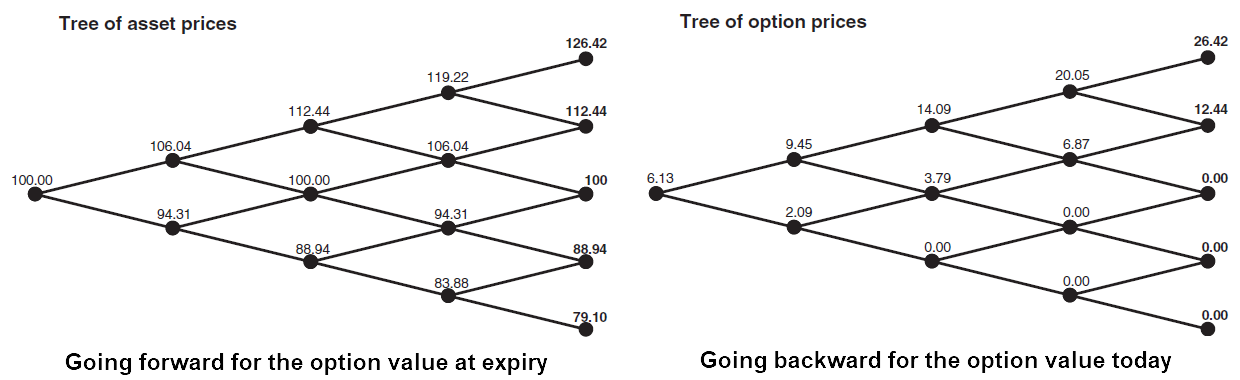
\includegraphics[width=\textwidth]{figure/binomial_tree.png} 
    \caption{The binomial tree}
    \label{fig:binomial_tree}
\end{figure}

The binomial tree also illustrate how to fully calculate the asset prices and the option prices. By going forward, one can find the option value at expiry $(V^+, V^-)$ at time $T$. As we know these values, we can find the option values one step further back in time. And by going backward to the root which is the current time and asset value, we can find the option value today. Programming of this process is given in Section \ref{sec:binomial_tree}

The aforementioned binomial setting is for European-style exercise. The algorithm of American-style exercise is identical with one exception  in the formula for $V$. We must ensure that there are no arbitrage opportunities at any of the nodes, i.e. the option value must be higher than the payoff value at any time.


\subsection{Miscellaneous}
The greeks are defined as derivatives of the option value with respect to various variables and parameters. These greeks will later be very important when we talk about risk management. It is important to distinguish whether the differentiation is with respect to a variable or a parameter (it could, of course, be with respect to both). If the differentiation is only with respect to the asset price and/or time then there is sufficient information in our binomial tree to estimate the derivative. It may not be an accurate estimate, but it will be an estimate. The option’s delta, gamma and theta, defined below can all be estimated from the tree. On the other hand, if you want to examine the sensitivity of the option with respect to one of the parameters, then you must perform another binomial calculation.

The binomial model can also lead us to the famous Black–Scholes equation. The binomial model is a discrete-time model whereas Black–Scholes is in continuous time.

The binomial method is just a simple version of an explicit finite-difference scheme. Finite-difference methods are far more flexible and can, in many ways, incorporate dividends, allow Bermudan exercise, value path-dependent contracts and price contracts depending on other stochastic variables such as interest rates. The binomial can also do these but in a more complicated way. 

Further remarks on risk neutrality by Paul Wilmott are given here:
\begin{itemize}
    \setlength\itemsep{0em}
    \item Hedging is used to eliminate risk.
    \item In simple models, hedging can be used to eliminate all risk from an option position.
    \item As well as eliminating risk, hedging removes dependence of an option value on the direction of an asset.
    \item If we don't care whether the asset price rises or falls, we shouldn't care about the probability of the rise or fall.
    \item \textit{The risk-neutral random walk is one that has the same volatility as the real asset random walk but a drift rate that is the same as the risk-free interest rate and not the real drift rate.}\footnote{Italic, here and down, means I still don't understand what Wilmott is talking about :).}
    \item \textit{The punchline is that the option value is the present value of the option payoff under a risk-neutral random walk}.
\end{itemize}



\section{Random behavior of assets}
\subsection{Jensen's inequality}
\textbf{Jensen's inequality}\index{Jensen's inequality} illustrates the importance of randomness in option theory. Let's look into the example below.

\begin{center}
\begin{footnotesize}
\fbox{
\begin{minipage}{0.90\textwidth}
The stock price is \$100 today. In one year's time, it could be \$50 or 150 with both equally likely. How can we value an option on this stock, e.g. a call option with a strike of 100 expiring in one year?

With those two possible scenarios we could say that we expect the stock price to be at \$100 in one year, this being the average of the possible future values. The payoff for the call option would then be 0, since it is exactly at the money. And the present value of this is zero.

Alternatively we could look at the two possible payoffs and then calculate that expectation. If the stock falls to 50 then the payoff is zero, if it rises to 150 then the payoff is 50. The average payoff is therefore 25, which we could present value to give us some idea of the option's value.

It turns out that the second calculation is closer to what we do in practice to value options although we know that the real probabilities don't come into the calculation. But that calculation illustrates another point of great importance, that the order in which we do the payoff calculation and the expectation matters, i.e.:
\begin{align}
    \text{Payoff} \left( \text{Expected} \left[ \text{Stock price} \right] \right) & = 0 \\
    \text{Expected} \left[ \text{Payoff} \left( \text{Stock price} \right) \right] & = 0     
\end{align}
This is an example of Jensen's inequality.

We can estimate how much the left-hand side is larger than the right-hand side. If we have a convex function $f(S)$ - the payoff function for a call of a random variable $S$ - the stock price then:
\begin{equation}
    E \left[ f \left( S \right) \right] \geq f \left( E \left[ S \right] \right)
\end{equation}

As $S$ is a random variable, let's assume that:
\begin{equation}
    S = E \left[ S \right] + \epsilon = \bar{S} + \epsilon
\end{equation}
in which $\bar{S}$ is the mean of $S$ and hence $E \left[ \epsilon \right] = 0$.

Now, we use the Taylor series approximation:
\begin{align}
    E \left[ f \left( S \right) \right] & = E \left[ f \! \left( \bar{S} + \epsilon \right) \right] = E \left[ f \! \left( \bar{S} \right) + \epsilon f' \! \left( \bar{S} \right) + \frac{1}{2} \epsilon^2 f'' \! \left( \bar{S} \right) \right] \\
    & \approx f \! \left( \bar{S} \right) + \frac{1}{2} f'' \! \left( \bar{S} \right) E \left[ \epsilon^2 \right] \\
    & = f \! \left[ E \left( S \right) \right] + \frac{1}{2} f'' \! \left( E \left[ S \right] \right) E \left[ \epsilon^2 \right]
\end{align}

$E \left[ \epsilon^2 \right]$ is the randomness in the underlying, and it variance. Modeling randomness is the key to modeling options.
\end{minipage}
}
\end{footnotesize}
\end{center}


\subsection{Returns}
This part is based on Chapter 4 of Wilmott \cite{pw_iqf2ed_2007}. When we invest in something, we would expect to have a comfortable return on our investment. By return, we mean the percentage growth in the value of an asset, together with accumulated dividends, over some period:
\begin{equation}
    \text{Return} = \frac{\text{change in value of the asset + accumulated cash flows}}{\text{original value of the asset}}
\end{equation}

When we model assets, it is the return that we should concentrate on. Part of the business of estimating returns for each asset is to estimate how much unpredictability there is in the asset value. It turns out that randomness plays a large part in financial markets \cite{pw_iqf2ed_2007}.

In modeling the returns, the following concepts, terms and processes are extremely important:
\begin{itemize}
    \setlength\itemsep{0em}
    \item The daily returns look very much like `noise' and is modeled as such. You, perhaps, have to wait months before you can spot the trend.
    \item The empirical returns are close enough to a random variable following the NORMAL distribution function with a non-zero mean and a non-zero standard deviation.
    \item The asset return model is similar to a model for a \textbf{random walk} of the asset price.
    \begin{equation}
        R_i = \frac{S_{i+1} - S_i}{S_i} = \mu \; \delta t + \sigma \; \phi \; \delta t^{1/2}
    \end{equation}
    or:
    \begin{equation}
        S_{i+1} = S_i \times \left(1 + \mu \; \delta t + \sigma \; \phi \; \delta t^{1/2} \right)
    \end{equation}    
    \item The parameter $\mu$ is called the drift rate, the expected return of the growth rate of the asset. In the classical option pricing theory, the drift plays almost no role. 
    \item The parameter $\sigma$ is called the volatility of the asset. The volatility is the most important and elusive quantity in the theory of derivatives. It is highly unlikely that volatility is constant for any given asset. Changing economic circumstances, seasonality, etc. will inevitably result in volatility changing with time.
    \item Because of their scaling with time, the drift and volatility have different effects on the asset path. The drift is not apparent over short timescales for which the volatility dominates. Over long timescales, for instance decades, the drift becomes important.
    \item The random walk model still have a discrete time step, this is a first step to develop a model in continuous-time. By changing from the normal distributions and discrete time to the \textbf{Wiener process}, the asset price model in the continuous-time limit using the Wiener process notation can be written as:
    \begin{equation}
        dS = \mu \; S \; dt + \sigma \; S \; dX
    \end{equation}
    This stochastic differential equation is a continuous-time model of an asset price. It is the most widely accepted model for equities, currencies, commodities and indices and the foundation of finance theory.
\end{itemize}
They will be described in more detailed in Section \ref{sec:randomness_assets}.
\chapter{Basic financial simulation I}
\cite{pw_optionpricing_1994, pw_mathfinderiv_1995, pw_derivatives_1998, pw_poqf2ed_2006, pw_iqf2ed_2007, mg_nmof_2019}

\section{Returns modeling}
\label{sec:randomness_assets}
Return is defined as the percentage growth in the value of an asset, together with accumulated dividends, over some period \citep{pw_iqf2ed_2007}:
\begin{equation}
    \text{Return} = \frac{\text{change in value of the asset + accumulated cash flows}}{\text{original value of the asset}}
\end{equation}

Denoting the asset value on the $i$-th day by $S_i$ then the return from day $i$ to day $i+1$ is given by:
\begin{equation}
     R_i = \frac{S_{i+1} - S_i}{S_i}
\end{equation}
The dividends are ignored here, they are easily allowed for, especially since they only get
paid two or four times a year typically. 

The mean of the returns distribution is:
\begin{equation}
    \text{mean} = \bar{R} = \frac{1}{M} \sum_{i = 1}^{M} R_i
    \label{equ:mean}
\end{equation}
and the sample standard deviation is:
\begin{equation}
    \text{sd} = \sqrt{\frac{1}{M-1} \sum_{i = 1}^{M} \left( R_i - \bar{R} \right)^2}
    \label{equ:std}
\end{equation}
where $M$ is the number of returns in the sample (one fewer than the number of asset prices). 

Figures \ref{fig:daily_return}(a,b) show the quoted price of a stock and its daily return in the duration considered. The daily return looks very much like `noise' and is modeled as such. Corresponding to the data in the example, the mean is 0.002916 and the standard deviation is 0.024521. Notice how the mean daily return is much smaller than the standard deviation. This is very typical of financial quantities over short timescales. On a day-by-day basis you will tend to see the noise in the stock price, and will have to wait months perhaps before you can spot the trend.

The frequency distribution of this time series of daily returns is plotted in Figure \ref{fig:daily_return}(c), it has been scaled and translated to give it a mean zero, a standard deviation of one and an area under the curve of one. This distribution is fairly close to the standardized normal distribution of
\begin{equation}
    \frac{1}{\sqrt{2\pi}} e^{-\frac{1}{2}\phi^2}
\end{equation}
where $\phi$ is a standardized normal variable.

Then, it is possible to assume that the returns can be modeled as a random variable drawn from a normal distribution with a know, constant, non-zero mean and a known, constant, non-zero standard deviation:
\begin{equation}
    R_i = \frac{S_{i+1} - S_i}{S_i} = \text{mean} + \text{sd} \times \phi
\end{equation}

\begin{figure}[H]
    \centering
    \begin{subfigure}[b]{0.3\textwidth}
        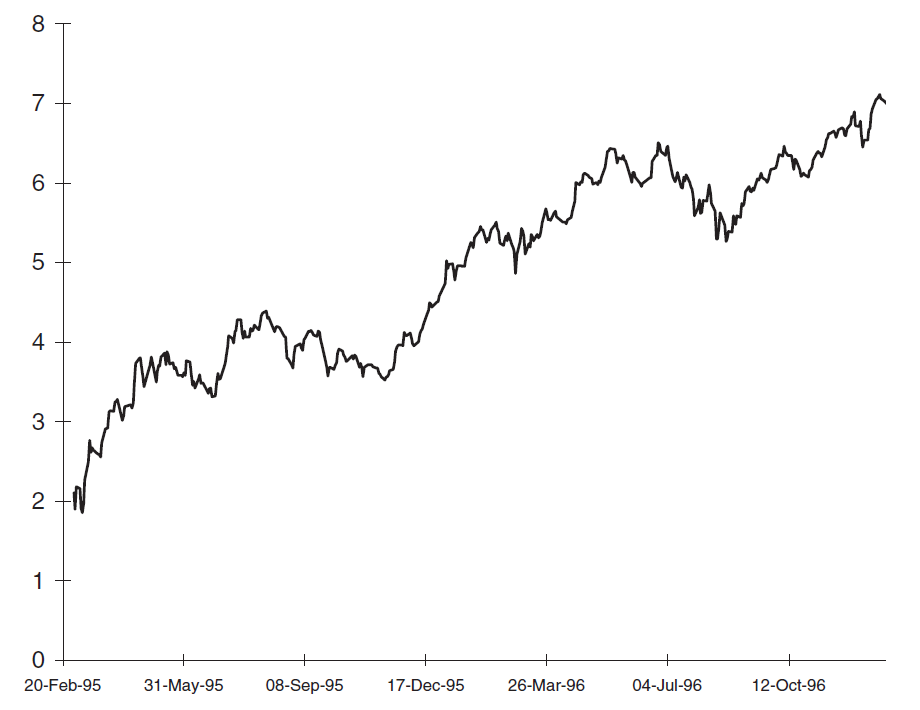
\includegraphics[width=\textwidth]{figure/daily_return_1.png}
        \caption{Quoted price of a stock}
    \end{subfigure}
    \begin{subfigure}[b]{0.3\textwidth}
        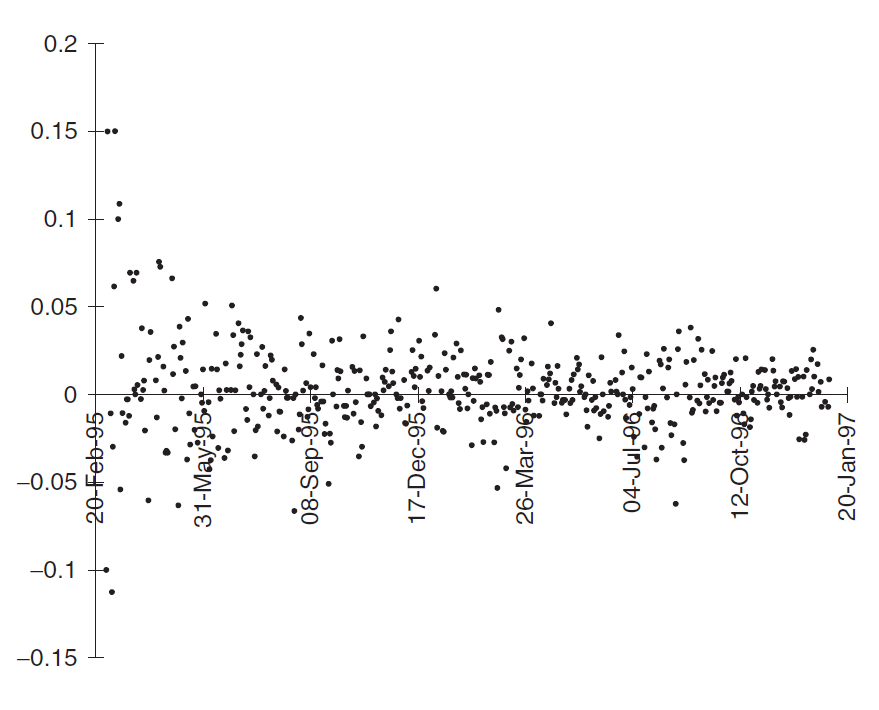
\includegraphics[width=\textwidth]{figure/daily_return_2.png}
        \caption{Daily returns}
    \end{subfigure}
    \begin{subfigure}[b]{0.3\textwidth}
        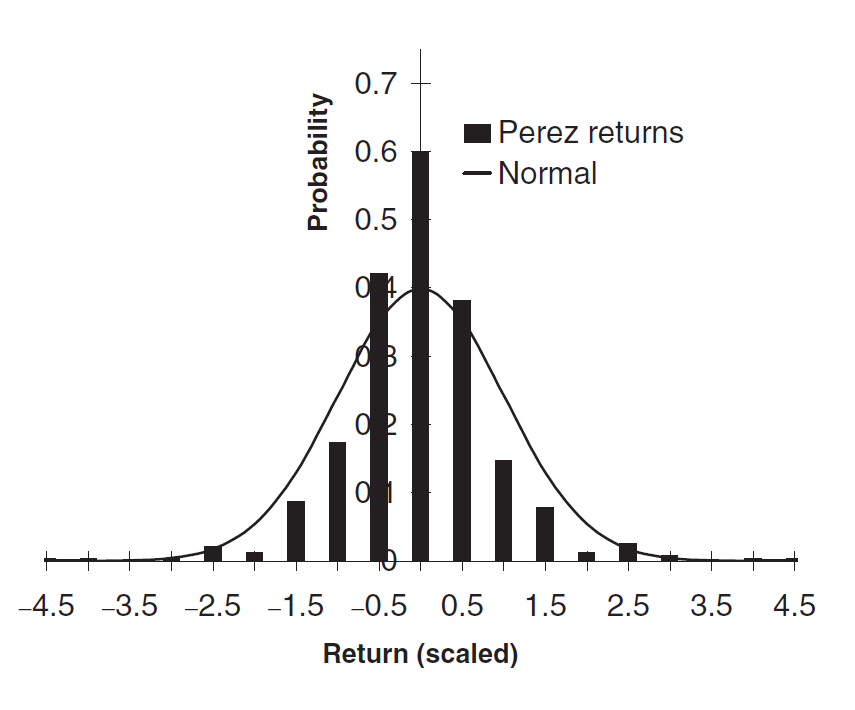
\includegraphics[width=\textwidth]{figure/daily_return_3.png}
        \caption{Norm. frequency distribution}
    \end{subfigure}
    \caption{Example of a daily return}
    \label{fig:daily_return}
\end{figure}



\subsection{Discrete-time model}
In reality, the assets may be measured in different time scale, i.e. hourly, daily, weekly... hence we need to take into account the time step in modeling returns. Call the time step $\delta t$. Following Equation \ref{equ:mean}, it is reasonable to assume that the return scales with the size of the time step as follows:
\begin{equation}
    \text{mean} = \mu \; \delta t
\end{equation}
for some $\mu$ which is assumed to be constant now. Similarly, following Equation \ref{equ:std}, the standard deviation of the asset return over a time step $\delta t$ must be $O \left( \delta t^{1/2} \right)$:
\begin{equation}
    \text{sd} = \sigma \; \delta t^{1/2}
\end{equation}
where $\sigma$ is some parameter measuring the amount of randomness, the larger this parameter the more uncertain is the return. And the asset return model becomes:
\begin{equation}
    R_i = \frac{S_{i+1} - S_i}{S_i} = \mu \; \delta t + \sigma \; \phi \; \delta t^{1/2}
\end{equation}
or:
\begin{equation}
    S_{i+1} - S_i = \mu \; S_i \; \delta t + \sigma \; S_i \; \phi \; \delta t^{1/2} 
\end{equation}   
The left-hand side of this equation is the change in the asset price from time step $i$ to time step $i+1$. The right-hand side is the `model'. We can think of this equation as a model for a \textbf{random walk}\index{random walk} of the asset price.

The parameter $\mu$ is called the \textbf{drift rate}\index{drift rate}, the \textbf{expected return}\index{expected return} or the \textbf{growth rate}\index{growth rate} of the asset. It can be estimated by:
\begin{equation}
    \mu = \frac{1}{M \delta t} \sum_{i = 1}^{M} R_i
    \label{equ:drift}
\end{equation}
Statistically it is very hard to measure since the mean scales with the usually small parameter $\delta t$. The unit of time that is usually used is the year, in which case $\mu$ is quoted as an annualized growth rate. In the classical option pricing theory the drift plays almost no role. So even though it is hard to measure, this doesn't matter too much \cite{pw_iqf2ed_2007}.

The parameter $\sigma$ is called the \textbf{volatility}\index{volatility} of the asset. It can be estimated by:
\begin{equation}
    \sigma = \sqrt{\frac{1}{\left( M - 1 \right) \delta t} \sum_{i = 1}^{M} \left( R_i - \bar{R} \right)^2}
    \label{equ:volatility_1}
\end{equation}
Again, this is almost always quoted in annualized terms. The volatility is the most important and elusive quantity in the theory of derivatives. If $\delta t$ is sufficiently small, the mean return $\bar{R}$ term can be ignored; and in this case, the following equation:
\begin{equation}
    \sigma = \sqrt{\frac{1}{\left( M - 1 \right) \delta t} \sum_{i = 1}^{M} \left( \log S(t_i) - \log S(t_{i-1}) \right)^2}
    \label{equ:volatility_2}
\end{equation}
can be used where $S(t_i)$ is the closing price on day $t_i$.

Because of their scaling with time, the drift and volatility have different effects on the asset path. The drift is not apparent over short timescales for which the volatility dominates. Over long timescales, for instance decades, the drift becomes important.

It is highly unlikely that volatility is constant for any given asset. Changing economic circumstances, seasonality, etc. will inevitably result in volatility changing with time. If
you want to know the volatility today you must use some past data in the calculation.  Unfortunately, this means that there is no guarantee that you are actually calculating today's volatility. Typically you would use daily closing prices to work out daily returns and then use the past 10, 30, 100, ... daily returns in the formula above.

\begin{figure}[H]
    \centering
    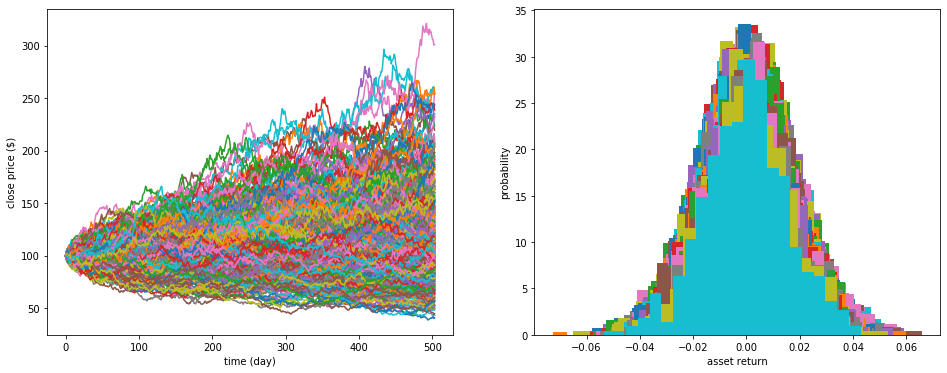
\includegraphics[width=\textwidth]{figure/random walk.png}
    \caption{Random walk model for an asset and corresponding return}
    \label{fig:random_walk_500}
\end{figure}

Figure \ref{fig:random_walk_500} reproduces the random walk model presented in Section 4.8 \cite{pw_iqf2ed_2007} for 500 evolution scenarios of an asset with the initial value of \$100, the drift rate $\mu$ of 0.10, the volatility $\sigma$ of 0.25, a daily quote in two-year duration. The corresponding asset returns of those 500 scenarios are also calculated, it can be seen that the asset returns closely follow the normal distribution as expected. Python code for this basic model can be found \href{https://github.com/chitn/quantfin_study/blob/master/code/asset_modeling-random_walk.py}{here}.



\subsection{Continuous-time model}
The random walk model described in the previous section has a discrete time step; in this section, a brief introduction to the continuous-time limit of the random walk model is presented as a starting point for the world of stochastic modeling and Wiener processes. These topics will be presented in more detailed in Section \ref{sec:stochastic_calculus}.

We rewrite the asset return model here for convenience:
\begin{equation}
    S_{i+1} - S_i = \mu \; S_i \; \delta t + \sigma \; S_i \; \phi \; \delta t^{1/2}
\end{equation}

First we introduce a quantity $dS$ representing \textit{the change in} the asset price in \textit{continuous time}, i.e. we go to the limit $\delta t = 0$. So the left-hand side becomes $dS$. The first $\delta t$ in the right-hand side can also translate into $dt$. 

For the second term of the right-hand side, however, we can not straightforwardly translate $\delta t^{1/2}$ into $dt^{1/2}$ \textit{otherwise any random $dt^{1/2}$ will dominate any deterministic $dt$ term}. It turns out, we will see in Section \ref{sec:stochastic_calculus}, that because the variance of the random term is $O(\delta t)$ we can make a sensible continuous-time limit of our discrete-time model. The term $\phi \delta t^{1/2}$ is rewritten as $dX$ which can be thought as a random variable drawn from a normal distribution with mean zero and variance $dt$, i.e. $E[dX] = 0$ and $E[dX^2] = dt$. This is called a Wiener process. It should be noted that \textit{this is not exactly what it is but it is close enough}, the important point is that we can build up a continuous-time theory using Wiener processes instead of normal distribution and discrete time. 

The asset price model in the continuous-time limit using the Wiener process notation can be written as:
\begin{equation}
    dS = \mu \; S \; dt + \sigma \; S \; dX
\end{equation}
This is our first stochastic differential equation. It is a continuous-time model of an asset price. It is the most widely accepted model for equities, currencies, commodities and indices, and the foundation of so much finance theory. This equation will be derived following different approaches in next sections.



\section{Elementary stochastic calculus}
\label{sec:stochastic_calculus}

Main references: \cite{pw_iqf2ed_2007}

\subsection{Introduction}
\textbf{Stochastic calculus}\index{stochastic calculus} is very important in the mathematical modeling of financial processes because of the underlying random nature of financial markets. This section provides a brief introduction to elementary stochastic calculus. 

This section will follow the methodology of chapter 5 of \cite{pw_iqf2ed_2007} in which technical terminologies are explained by examples relating to a \textbf{coin tossing}\index{coin tossing}, if possible, to make them intuitive. 

\begin{center}
\begin{footnotesize}
\fbox{
\begin{minipage}{0.90\textwidth}

Toss a coin. Every time you throw a head I give you \$1, every time you throw a tail you give
me \$1. If $R_i$ represents the random amount either \$1 or \$1 you make on the $i$-th toss then we have:
\begin{equation}
    E\left[ R_i \right] = 0, \quad E\left[ R_i^2 \right] = 1, \quad E\left[ R_i R_j \right] = 0
\end{equation}
These expectations are not conditional on the past; in other words, if I threw five heads in a row it does not affect the outcome of the sixth toss.

Introduce $S_i$ to represent the total amount of money you have won up and including the $i$-th toss so that:
\begin{equation}
    S_i = \sum_{j = 1}^{i} R_j
\end{equation}
and assume that $S_0 = 0$, i.e. you start with no money. If we calculate the expectations of $S_i$ it does matter what information we have:
\begin{equation}
    E\left[ S_i \right] = 0, \quad E\left[ S_i^2 \right] = E\left[ R_1^2 + 2R_1R_2 + ... \right] = i
\end{equation}
On the other hand, if there are five tosses already, then the expectation of the sixth toss will depends on the fifth tosses. This is the conditional expectation. The expectation of $S_i$ conditional upon the previous five tosses gives:
\begin{equation}
    E \left[ S_6 | R_1, R_2, ..., R_5 \right] = S_5
\end{equation}

\end{minipage}
}
\end{footnotesize}
\end{center}

The property that the expected value of the random variable $S_i$ \textit{conditional upon all of the past events only depends on the previous value} $S_{i-1}$ (doesn't have to be the case that the expected value of $S_i$ is equal to $S_{i-1}$) is called \textbf{Markov property}\index{Markov property}. We say that the random walk has no memory beyond where it is now. Almost all of the financial models have the Markov property. This is of fundamental importance in modeling in finance.

\begin{center}
\begin{footnotesize}
\fbox{
\begin{minipage}{0.90\textwidth}

After the fifth toss, you know how much money you have won. Your expected winnings after the sixth toss, and actually after any number of tosses if we keep playing, is just the amount you already hold.
\begin{equation}
    E \left[ S_i | R_j, j < i \right] = S_j
\end{equation}

\end{minipage}
}
\end{footnotesize}
\end{center}

The property that the conditional expectation of your winnings at any time in the future is just the amount you already hold is called the \textbf{martingale property}\index{martingale property}. This is another important property in finance.

The \textbf{quadratic variation}\index{quadratic variation} of the random walk is defined as:
\begin{equation}
    \sum_{j = 1}^i \left( S_j - S_{j-1} \right)^2
\end{equation}
Going back to the coin tossing example, because you either win or lose an amount \$1 after each toss, we actually have $\left| S_j - S_{j-1} \right| = 1$, thus the quadratic variation is always $i$.

The \textbf{mean square limit}\index{mean square limit} technique states that:
\begin{equation}
    E \left[ \left( \sum_{j=1}^n \left( X(t_j) - X(t_{j-1}) \right)^2 - t \right) \right] = O \left( \frac{1}{n} \right)
\end{equation}
as $n \rightarrow \infty$ this tends to zero. Therefore, we can say that:
\begin{equation}
    \sum_{j=1}^n \left( X(t_j) - X(t_{j-1}) \right)^2 = t
\end{equation}
in the `mean square limit'. This is often written as:
\begin{equation}
    \int_0^t (dX)^2 = t
\end{equation}



\subsection{Brownian motion}
\begin{center}
\begin{footnotesize}
\fbox{
\begin{minipage}{0.90\textwidth}

Now we make some changes in the coin tossing game: first, the time allowed for tossing is a period $t$; second, within the period $t$ we will perform $n$ tosses with the bet size of each throw is $\sqrt{t/n}$. This new experiment clearly still possesses both the Markov and martingale properties, and its quadratic variation measured over the whole experiment is:
\begin{equation}
    \sum_{j = 1}^n \left( S_j - S_{j-1} \right)^2 = n \times \left( \sqrt{\frac{t}{n}} \right)^2 = t
\end{equation}

To speed up the game, we will make $n$ larger and larger, i.e. decreasing the time between tosses, with a smaller amount for each bet, i.e. still keep the bet size of $\sqrt{t/n}$. You will see that as we go to the limit $n = \infty$, the resulting random walk stays finite. It has an expectation conditional on a starting value of zero and a variance of $t$:
\begin{align}
    E \left[ S(t) \right] &= 0 \\
    E \left[ S(t)^2 \right] &= t        
\end{align}

\end{minipage}
}
\end{footnotesize}
\end{center}

The limiting process for this random walk as the time steps go to zero is called \textbf{Brownian motion}\index{Brownian motion}, and it is denoted by $X(t)$. The important properties of Brownian motion, which are also very important for financial models, are as follows:
\begin{itemize}
    \setlength\itemsep{0em}
    \item \textbf{Finiteness}: any other scaling of the bet size or `increments' with time step would have resulted in either a random walk going to infinity in a finite time, or a limit in which there was no motion at all. It is important that the increment scales with the square root of the time step.
    \item \textbf{Continuity}: the paths are continuous, there are no discontinuities. Brownian motion is the continuous-time limit of our discrete time random walk.
    \item \textbf{Markov}: the conditional distribution of $X(t)$ given information up until $\tau < t$ depends only on $X(\tau)$.
    \item \textbf{Martingale}: given information up until $\tau < t$ the conditional expectation of $X(t)$ is $X(\tau)$.
    \item \textbf{Quadratic variation}: if we divide the time 0 to $t$ into $n+1$ partition points $t_i = it/n$ then:
    \begin{equation}
        \sum_{j = 1}^n \left( X \left( t_j \right) - X \left( t_{j-1} \right) \right)^2 \rightarrow t
    \end{equation}
    \item \textbf{Normality}: over finite time increments $t_{i-1}$ to $t_i$, $X \left( t_j \right) - X \left( t_{j-1} \right)$ is normally distributed with mean zero and variance $t_i - t_{i-1}$.
\end{itemize}


\subsection{Stochastic integration and differentiation}
Introductory calculus courses teach differentiation first and integration second. The Itô calculus is derived and taught in the reverse order:
first we need to understand the definition of an Itô (stochastic) integral, and then we can understand what it means for a stochastic process to have a differential.

The construction of the Itô integral begins with the backward Riemann sum:
\begin{equation}
    W(t) = \int_0^t f(\tau) \; dX(\tau) = \lim_{n \rightarrow \infty} \sum_{j=1}^{n} f \left( t_{j-1} \right) \; \left( X \left( t_j \right) - X \left( t_{j-1} \right) \right)
    \label{equ:itoo_001}
\end{equation}
with:
\begin{equation}
    t_j = \frac{jt}{n}
\end{equation}
The function $f(t)$ which is integrated is evaluated in the summation at the left-hand point $t_{j-1}$ which means each function evaluation does not know about the random increment that multiplies it, i.e. the integration is non \textbf{anticipatory}. This choice of integration is natural in finance, ensuring that we use no information about the future in our current actions.

Taking the ``differentiating'' of the first equation of Equation \ref{equ:itoo_001} we have:
\begin{equation}
    dW = f(t) \; dX
\end{equation}
$dX$ can be considered as an an increment in $X$, i.e. a normal random variable with mean zero and standard deviation $\sqrt{dt}$. This equation looks like an ordinary differential equation but we do not make it identical to the ODE by dividing by $dt$ because then we have the difficult task of defining $\frac{dX}{dt}$.

Pursuing this idea further, then the equation:
\begin{equation}
    dW = g(t) \; dt + f(t) \; dX
\end{equation}
is equivalent to:
\begin{equation}
    W(t) = \int_0^t g(\tau) \; d\tau + \int_0^t f(\tau) \; dX(\tau)
    \label{equ:sde}
\end{equation}
Equations like \ref{equ:sde} are called \textbf{stochastic differential equations (SDE)}\index{stochastic differential equations} \index{SDE}. 



\subsubsection{Itô's lemma}
We know that in deterministic calculus if $F = X^2$ then $dF = 2X \; dX$. However this rule is not applicable in a stochastic environment. \textbf{Itô's lemma}, the most important rule of stochastic calculus, is used for this purpose since it allows us to manipulate functions of a random variable. This section provides the derivation of the Itô's lemma for an arbitrary function $F(X)$.

First we introduce a very, very small time scale:
\begin{equation}
    \frac{\delta t}{n} = h
\end{equation}
This timescale is so small that the function $F(X(t+h))$ can be approximated by a Taylor series:
\begin{equation}
    F(X(t+h)) - F(X(t)) = (X(t+h) - X(t)) \; \frac{dF}{dX} (X(t)) + \frac{1}{2}(X(t+h) - X(t))^2 \; \frac{d^2F}{dX^2}(X(t))
\end{equation}
This can be followed as:
\begin{align}
    [F(X(t+h)) &- F(X(t))] + [F(X(t+2h)) - F(X(t+h))] + ... \nonumber \\
    &+ [F(X(t+nh)) - F(X(t+(n-1)h))] \nonumber \\
    &= \sum_{j=1}^n (X(t+jh) - X(t+(j-1))) \; \frac{dF}{dX} (X(t+(j-1)h)) \nonumber \\
    &+ \frac{1}{2} \; \sum_{j=1}^n (X(t+jh) - X(t+(j-1)))^2 \; \frac{d^2F}{dX^2}(X(t))
    \label{equ:itoo_002}
\end{align}
in which we use the approximation:
\begin{equation}
    \frac{d^2F}{dX^2}(X(t+(j-1)h)) = \frac{d^2F}{dX^2}(X(t))
\end{equation}
which is consistent with the order of accuracy we require here. 

The first term in Equation \ref{equ:itoo_002} can be rewritten as:
\begin{equation}
    F(X(t+nh)) - F(X(t)) = F(X(t+\delta t)) - F(X(t))
\end{equation}
the second term is just the definition of a normal integral:
\begin{equation}
    \sum_{j=1}^n (X(t+jh) - X(t+(j-1))) \frac{dF}{dX} (X(t+(j-1)h)) = \int_t^{t+\delta t}\frac{dF}{dX}dX
\end{equation}
and the last term, following the mean square limit (this will be presented later), can be shortened into:
\begin{equation}
    \frac{1}{2} \sum_{j=1}^n (X(t+jh) - X(t+(j-1)))^2 \frac{d^2F}{dX^2}(X(t)) = \frac{1}{2} \; \frac{d^2F}{dX^2}(X(t)) \; \delta t
\end{equation}
Finally we have:
\begin{equation}
    F(X(t+\delta t)) - F(X(t)) = \int_t^{t+\delta t}\frac{dF}{dX}(X(\tau)) \; dX(\tau) + \frac{1}{2} \int_t^{t+\delta t}\frac{d^2F}{dX^2}(X(\tau)) \; d\tau
\end{equation}
Now we extend this result over longer timescale, $0 \rightarrow t$, to get:
\begin{equation}
    F(X(t)) = F(X(0)) + \int_0^t \frac{dF}{dX}(X(\tau)) \; dX(\tau) + \frac{1}{2} \int_0^t \frac{d^2F}{dX^2}(X(\tau)) \; d\tau
\end{equation}
This is the integral version of \textbf{Itô's lemma}\index{Itô's lemma} which is usually written as:
\begin{equation}
    dF = \frac{dF}{dX} dX + \frac{1}{2} \frac{d^2F}{dX^2} dt
    \label{equ:itoo_003}
\end{equation}

Now if we look back at the naive Taylor series expansion of $F$, completely disregarding the random nature of $X$, and treating $dX$ as a small increment in $X$, we would get:
\begin{equation}
    F(X+dX) = F(X) + \frac{dF}{dX}dX + \frac{1}{2} \frac{d^2F}{dX^2}dX^2
\end{equation}
and if we consider $F(X+dX) - F(X)$ is just the change in $F$ we have:
\begin{equation}
    dF = \frac{dF}{dX}dX + \frac{1}{2} \frac{d^2F}{dX^2}dX^2
\end{equation}
This equation is very similar to Equation \ref{equ:itoo_003} (as Taylor series is very similar to Itô) with the only difference being that there is a $dX^2$ instead of a $dt$. However, following the mean square limit, we have:
\begin{equation}
    \int_0^t (dX)^2 = t
\end{equation}
we could write:
\begin{equation}
    dX^2 = dt
\end{equation}
This equation is technically incorrect, but using Taylor series with this ``rule of thumb'' in practice, we can get the right result. Besides, we shouldn't really think of $dX^2$ as being the square of a single normally distributed random variable, mean zero, variance $dt$. We should think of it as the sum of squares of lots and lots (an infinite number) of independent and identically distributed normal variables, each one having
mean zero and a very, very small (infinitesimal) variance. When we add together lots of i.i.d. variables, we will get a quantity with a mean of $dt$ and a variance which goes rapidly to zero as the `lots' approach `infinity'. 

\begin{center}
\begin{footnotesize}
\fbox{
\begin{minipage}{0.90\textwidth}

Now we can come back to the first example of this section, if $F=X^2$ then the stochastic differential equation of which $F$ satisfies is:
\begin{equation}
    dF = 2X \; dX + dt
\end{equation}
In an integrated form:
\begin{equation}
    X^2 = F(X) = F(0) + \int_0^t 2X \; dX + \int_0^t 1 d\tau = \int_0^t 2X \; dX + t
\end{equation}
therefore:
\begin{equation}
    \int_0^t X \; dX = \frac{1}{2} X^2 - \frac{1}{2} t
\end{equation}

\end{minipage}
}
\end{footnotesize}
\end{center}

To end this section, we consider the stochastic differential equation:
\begin{equation}
    dS = a(S) \; dt + b(S) \; dX
\end{equation}
for some functions $a(S)$ and $b(S)$, and $dX$ is the usual Brownian increment. Now if we have a function $V(S)$ of $S$, the stochastic differential equation applicable for $V$ is:
\begin{equation}
    dV = \frac{dV}{dS}dS + \frac{1}{2} b^2 \frac{d^2V}{dS^2}dt
\end{equation}
We can also further subtitute $dS$ into the above equation to get an equation for $dV$ in terms of the pure Brownian motion $X$:
\begin{equation}
    dV = \left( a(S)\frac{dV}{dS} + \frac{1}{2} b(S)^2 \frac{d^2V}{dS^2} \right) dt + b(S) \frac{dV}{dS} dX
\end{equation}



\subsubsection{Itô in higher dimensions}
In financial problem, we often have functions of one stochastic variable $S$ and a deterministic variable $t$ (time) as $V(S,t)$. If:
\begin{equation}
    dS = a(S,t) \; dt + b(S,t) \; dX
\end{equation}
then the increment $dV$ is given by:
\begin{equation}
    dV = \frac{\partial V}{\partial t} dt + \frac{\partial V}{\partial S} dS + \frac{1}{2} b^2 \frac{\partial^2 V}{\partial S^2} dt
\end{equation}
This shorthand notation for the correct integrated from is written in the form of partial instead of ordinary derivatives.

Occasionally, we have a function of two or more random variables, and time as well, i.e. $V(S_1,S_2,t)$. We will write the behaviour of $S_1$ and $S_2$ in the general form:
\begin{align}
    dS_1 &= a_1(S_1,S_2,t) \; dt + b_1(S_1,S_2,t) \; dX_1 \\
    dS_2 &= a_2(S_1,S_2,t) \; dt + b_2(S_1,S_2,t) \; dX_2
\end{align}
in which we have two Brownian increment $dX_1$ and $dX_2$. We can think of these variables as being normally distributed with variance $dt$ but they are \textit{correlated}. The correlation between these two random variables is called $\rho$ which can also be a function of $S_1$, $S_2$ and $t$ but must satisfy:
\begin{equation}
    -1 \leq \rho \leq 1
\end{equation} 
The `rule of thumb' for this case can be:
\begin{equation}
    dX_1^2 = dt \quad dX_2^2 = dt \quad dX_1 dX_2 = \rho dt
\end{equation}
Then Itô's lemma becomes:
\begin{equation}
    dV = \frac{\partial V}{\partial t} dt + \frac{\partial V}{\partial S_1} dS_1 + \frac{\partial V}{\partial S_2} dS_2 + \frac{1}{2} b_1^2 \frac{\partial^2 V}{\partial S_1^2} dt + \frac{1}{2} b_2^2 \frac{\partial^2 V}{\partial S_2^2} dt + \rho b_1 b_2 \frac{\partial V}{\partial S_1 \partial S_2}
\end{equation}



\subsection{Some common random walks}
In this section, a couple of common random walks will be presented. Recall that a stochastic differential equation model for variable $S$ has the general form:
\begin{equation}
    dS = \underline{\hspace{2cm}} dt + \underline{\hspace{2cm}} dX
\end{equation}
The part in front of the $dt$ is deterministic and the part in front of the $dX$ tells us how much randomness there is. Modelling is about choosing the functional form for the deterministic part and the functional form for the amount of randomness.


\subsubsection{Brownian motion with drift}
A Brownian motion with drift has the form:
\begin{equation}
    dS = \mu \; dt + \sigma \; dX
\end{equation}
The point to note about this model is that $S$ can go negative. This random walk would therefore not be a good model for many financial quantities, such as interest rates or equity prices. This stochastic differential equation can be integrated exactly to get"
\begin{equation}
    S(t) = S(0) + \mu \; t + \sigma \; (X(t) - X(0))
\end{equation}



\subsubsection{The lognormal random walk}
The lognormal random walk is similar to the Brownian with drift but the drift and randomness scale with $S$:
\begin{equation}
    dS = \mu \; S \; dt + \sigma \; S \; dX
\end{equation}
With this model, if $S$ starts out positive, it can never go negative, the closer that $S$ gets to zero, the smaller the increments $dS$. The integral form of this stochastic differential equation follows from the stochastic differential equation for $F(S) = \log S$ (that's why it has the name ``lognormal''):
\begin{equation}
    S(t) = S(0) e^{\left( \mu - \frac{1}{2}\sigma^2 \right)t + \sigma \; (X(t) - X(0))}
\end{equation}
This stochastic differential equation is particularly important in the modelling of many asset classes. And if we have some function $V(S, t)$ then from Itô it follows that :
\begin{equation}
    dV = \frac{\partial V}{\partial t} \; dt + \frac{\partial V}{\partial S} \; dS + \frac{1}{2} \sigma^2 S^2 \frac{\partial^2 V}{\partial S^2} \; dt
\end{equation}



\subsubsection{A mean-reverting random walk}
A typical mean-reverting random walk has the form:
\begin{equation}
    dS = (\nu - \mu S) \; dt + \sigma \; dX
\end{equation}
If $S$ is large, the negative coefficient in front of $dt$ means that $S$ will move down on average, if $S$ is small it rises on average. There is still no incentive for $S$ to stay positive in this random walk. Mean-reverting models are used for modeling a random variable that `isn't going anywhere'. That's why they are often used for interest rates, e.g. governmental bonds.



\subsection{Summary}
This section revisited the most important tool of the trade, Itô's lemma. If we think of $S$ as the value of an asset for which we have a stochastic differential equation, a `model', then we can handle functions of the asset, and ultimately value contracts such as options.

If we use Itô as a tool we do not need to know why or how it works, only how to use it. Then, with use, familiarity breeds, if not contempt, sufficient confidence to make you believe that you understand. Some nice remarks on Itô's lemma given by Paul Wilmott \cite{pw_iqf2ed_2007} are presented here:
\begin{itemize}
    \setlength\itemsep{0em}
    \item Stochastic differential equations are like recipes for generating random walks.
    \item If you have some quantity, i.e. $S$, that follows a random walk, then any function of $S$ is also going to follow a random walk.
    \item The answer for the question `What is the random walk for this function of S?' comes from applying something very like Taylor series but with some `rule of thumb':
    \begin{itemize}
    \setlength\itemsep{0em} 
        \item When you do the Taylor series expansion, only keep terms of size $dt$ or bigger $dt^{1/2}$ ($dt^2 = 0$).
        \item Every time you see a $dX^2$ term replace it with $dt$.
        \item All terms with $dX \cdot dt$ varnishes, i.e. $dX \cdot dt = 0$ .
    \end{itemize}
\end{itemize}  

Essentially all we require to successfully use the lemma is a rule of thumb, as explained in the text.



\subsection{Exercises}
This section represents some exercises from \cite{pw_iqf2ed_2007} to practice with stochastic calculus.


\subsubsection{Problem}
Given an Brownian motion $X(t)$, show that:
\begin{equation}
    \int_0^t X(\tau) \; dX(\tau) = \frac{1}{2} X^2(t) - \frac{1}{2}t
    \nonumber
\end{equation}

\begin{equation}
    \int_0^t \tau \; dX(\tau) = t \; X(t) - \int_0^t X(\tau) \; d\tau
    \nonumber
\end{equation}

\begin{equation}
    \int_0^t X^2(\tau) \; dX(\tau) = \frac{1}{3} X^3(t) - \int_0^t X(\tau) \; d\tau
    \nonumber
\end{equation}


\subsubsection{Problem}
Given a function $f(t)$ which is continuous and bounded on $[0,t]$, prove the integration by parts:
\begin{equation}
    \int_0^t f(\tau) \; dX(\tau) = f(t) \; X(t) - \int_0^t X(\tau) \; df(\tau)
\end{equation}


\subsubsection{Problem}
Find $u(W,t)$ and $v(W,t)$ where:
\begin{equation}
    dW(t) = u \; dt + v \; dX(t)
    \nonumber
\end{equation}
in three scenarios:
\begin{itemize}
    \setlength\itemsep{0em}
    \item $W(t) = X^2(t)$
    \item $W(t) = e^{X(t)} + t + 1$
    \item $W(t) = f(t) \; X(t)$
\end{itemize} 
and $f(t)$ is a bounded and continuous function.


\subsubsection{Problem}
If $S$ follows a lognormal random walk, use Itô's lemma to find the differential equations satisfied by:
\begin{itemize}
    \setlength\itemsep{0em}
    \item $f(S) = aS + b$
    \item $g(S) = S^n$
    \item $h(S,t) = S^n \; e^{mt}$
\end{itemize} 
where $a, b, m, n$ are constants.


\subsubsection{Problem}
If:
\begin{equation}
    dS = \mu \; S \; dt + \sigma \; S \; dX
    \nonumber
\end{equation}
use Itô's lemma to find the stochastic differential equation satisfied by $f(S) = \log(S)$.


\subsubsection{Problem}
The change in the share price satisfies:
\begin{equation}
    dS = A(S,t) \; dX + B(S,t) \; dt
    \nonumber
\end{equation}
for some functions $A, B$, find the stochastic differential equation satisfied by $f(S,t)$.


\subsubsection{Problem}
Two shares follow geometric Brownian motions as:
\begin{align*}
    dS_1 &= \mu_1 \; S_1 \; dt + \sigma_1 \; S_1 \; dX_1 \\
    dS_2 &= \mu_2 \; S_2 \; dt + \sigma_2 \; S_2 \; dX_2     
\end{align*}
The share price changes are correlated with correlation coefficient $\rho$, find the stochastic differential equation satisfied by a function $f(S_1,S_2)$.


















\section{Black-Scholes model} 
Main references: \cite{pw_mathfinderiv_1995, pw_iqf2ed_2007}.


\subsection{Black-Scholes equation}
This section describes and explains the basic building blocks of derivatives theory which are delta hedging and no arbitrage.

\subsubsection{A portfolio}
The option value $V$ can be written as:
\begin{equation}
    V(S,t \; ; \sigma, \mu \; ; E, T \; ; r)
\end{equation}
in which:
\begin{itemize}    
    \setlength\itemsep{0em}
    \item the asset price $S$ and the current time $t$ are variables;
    \item the drift $\sigma$ and the volatility $\mu$ are parameters associated with the asset price;
    \item the strike price $E$ and the date of expiry $T$ are parameters associated with the details of the particular contract;
    \item the interest rate $r$ is a parameter associated with the currency in which the asset is quoted.
\end{itemize}
For the moment, we will only write $V(S,t)$ to denote the option value.

Now, consider a portfolio of one long option position and a short position in some quantity $\Delta$ of the underlying and denote $\Pi$ as the value of that portfolio, we have:
\begin{equation}
    \Pi = V(S,t) - \Delta S
    \label{equ:bs_000}
\end{equation}
The term $\Delta S$ is the short asset position, therefore it has a minus sign. The quantity $\Delta$ will be some constant quantity of our choosing. 

Now, assume that the underlying asset follows a lognormal random walk:
\begin{equation}
    dS = \mu S dt + \sigma S dX
\end{equation}
The change in the value of the option from time $t$ to time $t+dt$ is due partly to the change in the option value and partly to the change in the underlying:
\begin{equation}
    d\Pi = dV - \Delta dS
\end{equation}
Notice that $\Delta$ has not changed during the time step, as we assumed. 

From Itô's lemma we have:
\begin{equation}
    dV = \frac{\partial V}{\partial t} dt + \frac{\partial V}{\partial S} dS + \frac{1}{2} \sigma^2 S^2 \frac{\partial^2 V}{\partial S^2} dt
\end{equation}
Thus, the portfolio changes by:
\begin{equation}
    d\Pi = \frac{\partial V}{\partial t} dt + \frac{\partial V}{\partial S} dS + \frac{1}{2} \sigma^2 S^2 \frac{\partial^2 V}{\partial S^2} dt - \Delta dS
    \label{equ:bs_001}
\end{equation}


\begin{center}
\begin{footnotesize}
\fbox{
\begin{minipage}{0.90\textwidth}

The binomial analysis seems to be easier to understand than the stochastic analysis of the Black–Scholes model. In principle they are nearly identical, it's just that the math is a more abstract with the Black–Scholes model. From a technical point of view, in the binomial model we did lots of modeling, hedging, etc. first before arriving at the Black–Scholes partial differential equation by performing a Taylor series expansion. In the Black–Scholes analysis the Taylor series expansion, in its stochastic form, comes first and the hedging,
etc. comes later.

\end{minipage}
}
\end{footnotesize}
\end{center}



\subsubsection{Delta hedging}
The right-hand side of Equation \ref{equ:bs_001} contains two types of terms, the deterministic terms being with $dt$ and the random terms being with $dS$. Assume that we know $V$ and its derivatives then we know everything on the right-hand side except for the value of $dS$. In fact we can never known this term in advance. The randomness terms are the risk in the portfolio. To reduce, or even eliminate this risk, we can, in theory and almost in practice, chose:
\begin{equation}
    \Delta = \frac{\partial V}{\partial S}
    \label{equ:bs_002}
\end{equation}
then the randomness reduces to zero. Any reduction in randomness is generally termed \textbf{hedging}. The perfect elimination of risk, by exploiting correlation between two instruments (in this case an option and its underlying), is generally called \textbf{delta hedging}. Delta hedging is an example of a \textbf{dynamic hedging} strategy. From one time step to the next, the quantity $\frac{\partial V}{\partial S}$ changes therefore the perfect hedge must be continually rebalanced. 



\subsubsection{No arbitrage}
After choosing the quantity $\Delta$, we hold a portfolio whose value changes by the amount:
\begin{equation}
    d\Pi = \left( \frac{\partial V}{\partial t} + \frac{1}{2} \sigma^2 S^2 \frac{\partial^2 V}{\partial S^2} \right) dt
    \label{equ:bs_003}
\end{equation}
This change is completely riskless. And in that case, the completely risk-free change $d\Pi$ must be the same as the growth we would get if we put the equivalent amount of cash in a risk-free interest-bearing account (i.e. the money-in-the-bank equation):
\begin{equation}
    d\Pi = r \Pi dt
    \label{equ:bs_004}
\end{equation}
This is an example of the \textbf{no-arbitrage} principle.



\subsubsection{Black-Scholes equation}
Substituting Equations \ref{equ:bs_000}, \ref{equ:bs_002} and \ref{equ:bs_003} into \ref{equ:bs_004} we find that;
\begin{equation}
    \left( \frac{\partial V}{\partial t} + \frac{1}{2} \sigma^2 S^2 \frac{\partial^2 V}{\partial S^2} \right) dt = r \left( V - S \frac{\partial V}{\partial S} \right) dt
\end{equation}
Dividing by $dt$ and rearranging we get:
\begin{equation}
    \frac{\partial V}{\partial t} + \frac{1}{2} \sigma^2 S^2 \frac{\partial^2 V}{\partial S^2} + rS \frac{\partial V}{\partial S} - rV = 0
    \label{equ:bs_original}
\end{equation}
This is the Black–Scholes equation published in 1973 by Fischer Black and Myron Scholes. The Black–Scholes equation contains all the obvious variables and parameters such as the underlying $S$, time $t$, and volatility $\sigma$, but there is no mention of the drift rate $\mu$ since it is dropped out at the same time as we eliminated the $dS$ component of the portfolio.

The Black–Scholes equation equation is a \textbf{linear} \textbf{parabolic} \textbf{partial differential equation}. 
\begin{itemize}
    \item As a linear function, if you have two solutions of the equation then the sum of these is itself also a solution.
    \item As a parabolic PDE (since it has a second derivative with respect to one variable, $S$, and a first derivative with respect to the other, $t$), it is related to the heat or diffusion equation of mechanics.
\end{itemize}   

The Black–Scholes equation can be accurately interpreted as a reaction-convection diffusion equation \cite{pw_iqf2ed_2007}. The basic diffusion equation is a balance of a first-order $t$ derivative and a second-order $S$ derivative:
\begin{equation}
    \frac{\partial V}{\partial t} + \frac{1}{2} \sigma^2 S^2 \frac{\partial^2 V}{\partial S^2} 
    \nonumber
\end{equation}
However, the diffusion coefficient is a function of one of the variables $S$, thus we really have diffusion in a non-homogeneous medium.

The first order $S$-derivative term:
\begin{equation}
    rS \frac{\partial V}{\partial S}
    \nonumber
\end{equation}
can be thought of as a convection term. For example, if this equation represents the diffusion of smoke particles in the atmosphere, then the convective term would be due to a wind blowing the smoke in a preferred direction.

The final term:
\begin{equation}
    -rV
    \nonumber
\end{equation}
is a reaction term. Balancing this term and the time derivative would give a model for decay of a radioactive body, with the half-life being related to $r$.

Putting these terms together and we get a reaction-convection-diffusion equation. An almost identical equation would be arrived at for the dispersion of pollutant along a flowing river with absorption by the sand. In this, the dispersion is the diffusion, the flow is the convection, and the absorption is the reaction \cite{pw_iqf2ed_2007}.



\subsection{Initial/final and boundary conditions}
To uniquely specify a problem we must prescribe boundary conditions and an initial or final condition. Boundary conditions tell us how the solution must behave for all time at certain values of the asset. 

In financial problems we usually specify the behavior of the solution at $S = 0$ and as $S \rightarrow \infty$. We must also tell the problem how the solution begins, i.e. a \textbf{initial condition}\index{initial condition}. The Black–Scholes equation is a backward equation, meaning that the signs of the $t$ derivative and the second $S$ derivative in the equation are the same when written on the same side of the equals sign. We therefore have to impose a \textbf{final condition}\index{final condition}. This is usually the payoff function at expiry.

Besides, the Black-Scholes equation \ref{equ:bs_original} knows nothing about what kind of option we are valuing, whether it is a call or a put, nor what is the strike and the expiry. These points are dealt with by, also, the final condition. We must specify the option value $V$ as a function of the underlying at the expiry date $T$, i.e. prescribing the payoff $V(S,T)$.
\begin{itemize}
    \setlength\itemsep{0em}
    \item For a call option:
    \begin{equation}
        V(S,T) = \max(S - E, 0)
    \end{equation}
    \item For a put option:
    \begin{equation}
        V(S,T) = \max(E - S, 0)
    \end{equation}
    \item For a binary call:
    \begin{equation}
        V(S,T) = \mathcal{H}(S - E, 0)
    \end{equation}
    in which $\mathcal{H}(x)$ is the \textbf{Heaviside function}\index{Heaviside function} which is zero when its argument is negative and one when it is positive.
    \item For a binary put:
    \begin{equation}
        V(S,T) = \mathcal{H}(E - S, 0)
    \end{equation}
\end{itemize}



\subsection{Some other ways of deriving Black-Scholes equation}
The derivation of the Black–Scholes equation above is the classical one, and similar to the original Black and Scholes derivation. There are other ways of getting to the same result. Here are a few approaches without any details \cite{pw_iqf2ed_2007}:
\begin{itemize}
    \setlength\itemsep{0em}
    \item The binomial model is a discrete time, discrete asset price model for underlying and again uses hedging and no arbitrage to derive a pricing algorithm for options. In taking the limit as the time step shrinks to zero we get the continuous-time Black–Scholes equation. We will see this derivation later.
    \item The martingale approach \footnote{The martingale approach follows the idea that the value of an option can be shown to be an expectation, not a real expectation but a special, risk-neutral one; this result forms the basis for pricing by simulation. The concepts of hedging and no arbitrage are still used in this derivation. The major drawback with this approach is that it requires a probabilistic description of the financial world}.  
    \item Capital Asset Pricing Model \footnote{CAPM is a model for the behavior of risky assets and a principle and algorithm for defining and finding optimal ways to allocate wealth among the assets. Portfolios are described in terms of their risk (standard deviation of returns) and reward (expected growth). If you include options in this framework then the possible combinations of risk and reward are not increased. This is because options are just functions of their underlyings. This is market completeness. The risk and reward on an option and on its underlying are related and the Black–Scholes equation follows}.
\end{itemize}

\textit{I haven't studied the two later approaches mentioned above, just name them here as examples.} More details information on those approaches can be found in \cite{ja_bsderivation_1998}.



\subsection{Forward and future contracts}
\subsubsection{Forward contracts}
Let $V(S,t)$ be the value of the forward contract at any time during its life on the underlying asset $S$ and maturing at time $T$. Set up the portfolio of one long forward contract and short $\Delta$ of the underlying asset:
\begin{equation}
    \Pi = V(S,t) - \Delta S
\end{equation}
From time $t$ to $t+dt$, this change by an amount:
\begin{equation}
    d\Pi = \frac{\partial V}{\partial t} dt + \frac{1}{2} \sigma^2 S^2 \frac{\partial^2 V}{\partial S^2} dt + \frac{\partial V}{\partial S} dS - \Delta dS 
\end{equation}
To eliminate risk, again we choose:
\begin{equation}
    \Delta = \frac{\partial V}{\partial S}
\end{equation} 
and by applying the no-arbitrage argument, we end up with exactly the Black-Scholes PDE again.

The final condition for the equation is simply the difference between the asset price $S$ and the fixed delivery price $\bar{S}$ - assumed for now that we know it, therefore:
\begin{equation}
    V(S,t) = S - \bar{S}
\end{equation}

The solution of the Black-Scholes with this final condition is:
\begin{equation}
    V(S,t) = S - \bar{S} e^{-r(T-t)}
\end{equation}
This is the forward contract's value during its life. 

Now we will calculate back $\bar{S}$. The delivery price is set initially $t = t_0$ as the price that gives the forward contract zero value. If the underlying asset is $S_0$ at $t_0$ then:
\begin{equation}
    0 = S_0 - \bar{S} e^{-r(T-t_0)}
\end{equation}
or:
\begin{equation}
    \bar{S} = S_0 e^{-r(T-t_0)}
\end{equation}

The forward price, as quoted, is the delivery price, as varying from day to day. So the forward price for the contract maturing at $T$ is:
\begin{equation}
    S \; e^{r(T-t)}
\end{equation}



\subsubsection{Future contracts}
Let $F(S,t)$ denote the futures price. Remember that the value of the futures contract during its life is always zero because the change in value is settled daily, this cash flow must be taken into account in our analysis. Therefore, if we set up a portfolio of one long futures contract and short $\Delta$ of the underlying, we have the value of that portfolio is:
\begin{equation}
    \Pi = \Delta S
\end{equation}
The portfolio change in value is:
\begin{equation}
    d\Pi = dF - \Delta dS
\end{equation}
in which $dF$ represents the cash flow due to the continual settlement. Applying the Itô's lemma we have:
\begin{equation}
    d\Pi = \frac{\partial F}{\partial t} dt + \frac{1}{2} \sigma^2 S^2 \frac{\partial^2 F}{\partial S^2} dt + \frac{\partial F}{\partial S} dS - \Delta dS
\end{equation}

Again, applying the hedging and no-arbitrage argument, i.e.:
\begin{equation}
    \Delta = \frac{\partial V}{\partial S} \quad \text{and} \quad d\Pi = r \Pi dt
\end{equation}
to get:
\begin{equation}
    \frac{\partial F}{\partial t} + \frac{1}{2} \sigma^2 S^2 \frac{\partial^2 F}{\partial S^2} + r S \frac{\partial F}{\partial S} = 0
\end{equation}
This equation has only three terms and it is not the same as the Black-Scholes equation.

The final condition is:
\begin{equation}
    F(S,T) = S
\end{equation}
indicating that the future price and the underlying must have the same value at maturity. The solution is just:
\begin{equation}
    F(S,t) = S e^{r(T-t)}
\end{equation}



\subsection{Some popular options}
\subsubsection{Option on dividend-paying equities}
The first generalization we discuss is how to value options on stocks paying dividends. To keep things simple let's assume that the asset receives a continuous and constant dividend yield $D$. Thus in a time $dt$ each asset receives an amount $DS dt$. This must be factored into the derivation of the Black–Scholes equation. 

The change in the value of the portfolio is given by:
\begin{equation}
    d\Pi = \frac{\partial V}{\partial t} dt + \frac{1}{2} \sigma^2 S^2 \frac{\partial^2 V}{\partial S^2} dt + \frac{\partial V}{\partial t} dS - \Delta dS - D \Delta S dt
\end{equation}
in which the last term is the amount of the dividend per asset $D S dt$ multiplied by the number of the asset held $-\Delta$. The $\Delta$ is still given by the rate of change of the option value with respect to the underlying, and after some simple substitutions we now get:
\begin{equation}
    \frac{\partial V}{\partial t} + \frac{1}{2} \sigma^2 S^2 \frac{\partial^2 V}{\partial S^2} + (r-D) S \frac{\partial V}{\partial S} - r V = 0
\end{equation}



\subsubsection{Currency options}
Options on currencies are handled in exactly the same way. In holding the foreign currency we receive interest at the foreign rate of interest $r_f$. This is just like receiving a continuous dividend, and we also have:
\begin{equation}
    \frac{\partial V}{\partial t} + \frac{1}{2} \sigma^2 S^2 \frac{\partial^2 V}{\partial S^2} + (r-r_f) S \frac{\partial V}{\partial S} - r V = 0
\end{equation}



\subsection{Main solution methods}
The three main mathematical approaches to derivative pricing are differential equations; binomial trees and expectations. All of these methods are based on pretty much the same assumptions. All of them will therefore give the same values for a contract, if all parameter values are the same. 

Analytical solutions for the Black-Scholes equation are rather complicated. A few techniques can be listed here for references \cite{pw_iqf2ed_2007}:
\begin{itemize}
	\setlength\itemsep{0em}
	\item Transformation to constant coefficient diffusion equation (see on the exercise section)
	\item Green's functions
	\item Series solutions
	\item Similarity reduction
	\item Fourier transforms
	\item Laplace transforms
\end{itemize} 
Analytical techniques, actually, can be used to solve only a small number of realistic financial problems; therefore you won't need to find explicit solutions. In practice, in the vast majority of cases we must solve the Black–Scholes equation numerically.   

Speaking of numerical methods, each of the three approaches has its own associated numerical method. Differential equations, and the Black–Scholes equation, in particular, can be solved by finite-difference methods. The binomial tree model is, interestingly, also its own numerical method. Finally, pricing by calculating risk-neutral expectations can be solved with Monte Carlo simulations. These three methods will be briefly described in this note.



\subsection{Exercises}
This section represents some exercises from \cite{pw_iqf2ed_2007} to practice with stochastic calculus.

\subsubsection{Problem}
Check that the following are solutions of the Black-Scholes equation:
\begin{itemize}
    \setlength\itemsep{0em}
    \item $V(S,t) = S$
    \item $V(S,t) = e^{rt}$
\end{itemize}


\subsubsection{Problem}
What is the most general solution of the Black-Scholes equation with each of the following forms:
\begin{itemize}
    \setlength\itemsep{0em}
    \item $V(S,t) = A(S)$
    \item $V(S,t) = B(S) \times C(t)$
\end{itemize}
i.e. find the most general form of functions $A, B$ and $C$.


\subsubsection{Problem}
Given an European call options $C(S,t)$ with expiry at time $T$ on an underlying share price $S$ with no dividends, prove the following bounds:
\begin{itemize}
    \setlength\itemsep{0em}
    \item $C \leq S$
    \item $C \geq \max(S-Ee^{-r(T-t)})$
    \item $0 \leq C_1 - C_2 \leq (E_2 - E_1) e{-r(T-t)}$
\end{itemize}
where $C_1, C_2$ are calls with exercise prices $E_1, E_2$, respectively and $E_1 < E_2$.


\subsubsection{Problem}
Given an European put options $P(S,t)$ with expiry at time $T$ on an underlying share price $S$ with no dividends, prove the following bounds:
\begin{itemize}
    \setlength\itemsep{0em}
    \item $P \leq Ee^{-r(T-t)}$
    \item $P \geq Ee^{-r(T-t)} - S$
    \item $0 \leq P_2 - P_1 \leq (E_2 - E_1) e{-r(T-t)}$
\end{itemize}
where $P_1, P_2$ are puts with exercise prices $E_1, E_2$, respectively and $E_1 < E_2$.


\subsubsection{Problem}
Given an European call options $C(S,t)$ on an underlying share price $S$ with no dividends, prove the following bounds:
\begin{itemize}
    \setlength\itemsep{0em}
    \item for $C_A$ and $C_B$ are calls with the same exercise price $E$ and expiry dates $T_A$ and $T_B$, respectively and $T_A > T_B$
    \begin{equation}
        C_A \geq C_B
    \end{equation}
    \item for $C_1, C_2$ and $C_3$ are calls with the same expiry $T$ and have exercise prices $E_1, E_2$ and $E_3$, respectively, and $E_1 < E_2 < E_3$
    \begin{equation}
        C_2 \leq \frac{E_3 - E_2}{E_3 - E_1} C_1 + \frac{E_2 - E_1}{E_3 - E_1} C_3
    \end{equation}
    Hint: consider a portfolio of $\Pi = \alpha C_1 - C_2 + (1-\alpha) C_3$.
\end{itemize}


\subsubsection{Problem}
Given $C(S,t)$ and $P(S,t)$ are the values of European call and put options with exercise price $E$ and expiry at time $T$. Show that a portfolio of long the call and short the put satisfies the Black-Scholes equation. What boundary and final conditions hold for this portfolio ?


\subsubsection{Problem}
Find the random walk followed by a European option $V(S, t)$. Use Black–Scholes to simplify the equation for $dV$.


\subsubsection{Problem}
Check that $u_\delta$ satisfies the diffusion equation where:
\begin{equation}
    u_\delta = \frac{1}{2\sqrt{\pi \tau}} e^{-\frac{x^2}{4 \tau}}
\end{equation}


\subsubsection{Problem}
Solve the Black-Scholes equation by transformation to constant coefficient diffusion equation (a change of variables technique) as:
\begin{itemize}
    \setlength\itemsep{0em}
    \item Set:
    \begin{equation}
        V(S,t) = e^{\alpha x + \beta \tau} U(x,\tau)
    \end{equation}
    in which:
    \begin{align*}
        \alpha &= -\frac{1}{2} \left( \frac{2r}{\sigma^2} - 1 \right)   \\
        \beta  &= -\frac{1}{4} \left( \frac{2r}{\sigma^2} + 1 \right)^2 \\
        S      &= e^{x}                                                 \\
        t      &= T - \frac{2\tau}{\sigma^2}
    \end{align*}
    \item Then $U(x,\tau)$ satisfies the basic diffusion equation:
    \begin{equation}
        \frac{\partial U}{\partial \tau} = \frac{\partial^2 U}{\partial x^2}
    \end{equation}
\end{itemize}
The solution for this problem will be described in the next section. 


\subsubsection{Problem}
Consider an option with value $V(S, t)$ which has payoff at time $T$. Reduce the Black–Scholes equation, with final and boundary conditions, to the diffusion equation, using the following transformations:
\begin{align*}
    S         &= e^{x}                               \\
    t         &= T - \frac{2\tau}{\sigma^2}          \\
    V(S,t)    &= EV(x,\tau)                          \\
    v(x,\tau) &= e^{\alpha x + \beta \tau} u(x,\tau)
\end{align*}
for some $\alpha$ and $\beta$. What is the transformed payoff? What are the new initial and boundary conditions? Illustrate with a vanilla European call option.


\subsubsection{Problem}
Reduce the following parabolic equation to the diffusion equation:
\begin{equation}
    \frac{\partial u}{\partial \tau} = \frac{\partial^2 u}{\partial x^2} + a \frac{\partial u}{\partial x} + b
\end{equation}
where $a$ and $b$ are constants. 


\subsubsection{Problem}
Using a change of time variable, reduce:
\begin{equation}
    c(\tau) \frac{\partial u}{\partial \tau} = \frac{\partial^2 u}{\partial x^2}
\end{equation}
to the diffusion equation when $c(\tau) > 0$.

Consider the Black–Scholes equation, when $\sigma$ and $r$ can be functions of time, but $k = 2r/\sigma^2$ is still a constant. Reduce the Black–Scholes equation to the diffusion equation in this case.



\section{Black-Scholes formul{\ae} and Greeks}

\subsection{Derivation for calls, puts and simple digitals}
The Black–Scholes equation has simple solutions for calls, puts and binary options whose payoff is a known function of the asset price at expiry. In this section, such solutions are presented. These will serve as the verification for the numerical solutions later. 

The Black-Scholes equation is:
\begin{equation}
    \frac{\partial V}{\partial t} + \frac{1}{2} \sigma^2 S^2 \frac{\partial^2 V}{\partial S^2} + r S \frac{\partial V}{\partial S} - r V = 0
    \label{equ:black-scholes-sol}
\end{equation}
which holds for $S > 0$ with $t \in [0, T)$. This equation must be solved with final condition depending on the payoff, i.e. $V(S,T) = \text{payoff of the derivatives}$, each contract will have a different functional form prescribed at expiry $t = T$.

The main steps to solve the Black-Scholes equation consist of:
\begin{enumerate}
	\setlength\itemsep{0em}
    \item change variable from present value to future value terms: since the payoff is received at time $T$ but we are valuing the option at time $t$, we can write:
    \begin{equation}
        V(S,t) = e^{-r(T-t)} U(S,t)
    \end{equation}    
    This makes Equation \ref{equ:black-scholes-sol} becomes:
    \begin{equation}
        \frac{\partial U}{\partial t} + \frac{1}{2} \sigma^2 S^2 \frac{\partial^2 U}{\partial S^2} + r S \frac{\partial U}{\partial S} = 0
    \end{equation}
    \item change time from $t$ to $\tau = T - t$ as we are solving a backward equation to make the equation becomes:
    \begin{equation}
        \frac{\partial U}{\partial \tau} = \frac{1}{2} \sigma^2 S^2 \frac{\partial^2 U}{\partial S^2} + r S \frac{\partial U}{\partial S}
    \end{equation}
    \item change variable from $S$ to $\xi = \log(S)$ to make all of the coefficients in the equation constant, independent of the underlying, we get:
    \begin{equation}
        \frac{\partial}{\partial S} = e^{-\xi}\frac{\partial}{\partial \xi} \quad \frac{\partial^2}{\partial S^2} = e^{-2\xi}\frac{\partial^2}{\partial \xi^2} - e^{-2\xi}\frac{\partial}{\partial \xi}
    \end{equation}
	and Equation \ref{equ:black-scholes-sol} becomes:
	\begin{equation}
	    \frac{\partial U}{\partial \tau} = \frac{1}{2} \sigma^2 \frac{\partial^2 U}{\partial \xi^2} + \left( r - \frac{1}{2} \sigma^2 \right) \frac{\partial U}{\partial \xi}
	\end{equation}
	This is a big step forward thanks to the lognormality of the underlying asset. 
    \item translate the coordinate system:
    \begin{align}
        x      &= \xi + \left( r - \frac{1}{2} \sigma^2 \right) \tau \\
        U(S,t) &= W(x,\tau)
    \end{align} 
    to make Equation \ref{equ:black-scholes-sol} becomes the standard heat equation which the solution can traditionally be found:
    \begin{equation}
        \frac{\partial W}{\partial \tau} = \frac{1}{2} \sigma^2 \frac{\partial^2 W}{\partial x^2}
        \label{equ:bs-heat}
    \end{equation}
\end{enumerate}

Those steps above can be summarised as follows:
\begin{align*}
    V(S,t) &= e^{-r(T-t)} U(S,t) \\
           &= e^{-r \tau} U(S,T - \tau) \\
           &= e^{-r \tau} U(e^{\xi},T - \tau) \\
           &= e^{-r \tau} U \left( e^{x - \left( r - \frac{1}{2} \sigma^2 \right) \tau},T - \tau \right) \\
           &= e^{-r \tau} W(x, \tau)
\end{align*}

We interest in a special solution of Equation \ref{equ:bs-heat} which has the following form:
\begin{equation}
    W(x,\tau) = \frac{1}{\sqrt{2 \pi \tau} \sigma}e^{-\frac{(x-x')^2}{2 \sigma^2 \tau}}
\end{equation}
where $x'$ is an arbitrary constant. The reason for this interest is explained in \citep{pw_iqf2ed_2007}.

Now, as the payoff $\text{Payoff}(S)$ is the value of the option at time $t = T$, we can write:
\begin{equation}
    V(S,T) = \text{Payoff}(S)
\end{equation}
and this is also the final condition for the function $V$ satisfying the Black-Scholes equation. In the equation of the new variables, this final condition is:
\begin{equation}
    W(x,0) = \text{Payoff}(e^x)
\end{equation}
The solution of this for $\tau > 0$ is:
\begin{align}
    W(x, \tau) &= \int_{-\infty}^{\infty} W(x, \tau, x') \text{Payoff}(e^{x'}) dx' \\ 
               &= \int_{-\infty}^{\infty} \frac{1}{\sqrt{2 \pi \tau} \sigma}e^{-\frac{(x-x')^2}{2 \sigma^2 \tau}} \text{Payoff}(e^{x'}) dx'
\end{align}

If we now come back to the original variables then the solution becomes:
\begin{equation}
    V(S,t) = \frac{e^{-r(T-t)}}{\sigma \sqrt{2 \pi (T-t)}} \int_0^\infty e^{-\frac{\left( \log(\frac{S}{S'}) + \left( r - \frac{1}{2} \sigma^2 \right)(T-t) \right)^2}{2 \sigma^2 (T-t)}} \; \text{Payoff}(S') \; \frac{dS'}{S'}
    \label{equ:exact_bsm}
\end{equation}
where we have written $x' = \log(S')$. This is the exact solution for the option value in terms of the arbitrary payoff function.

Before moving to some special payoff functions, let take a break by looking at the integral of the form:
\begin{equation}
    \int_a^\infty e^{-\frac{1}{2}x^2} dx
    \label{equ:cdf_bsm_01}
\end{equation}
for some $a$. This integral is rather similar to the cumulative distribution function for the standardized normal distribution defined by:
\begin{equation}
    N(x) = \frac{1}{\sqrt{2\pi}}\int_{-\infty}^x e^{-\frac{1}{2}\phi^2} d\phi
    \label{equ:cdf_bsm_02}
\end{equation}
This function is the probability that a normally distributed variable is less than $x$. You will see, later, that this $N(x)$ function is used alot in the solution of different payoff functions. The derivative of $N(x)$ is:
\begin{equation}
    N'(x) = \frac{1}{\sqrt{2\pi}} e^{-\frac{1}{2}x^2}
\end{equation}

To calculate $N(x)$, we can use the following formula which gives an accurate, and fast, approximation to the cumulative distribution function of the standardized normal distribution. For $x > 0$:
\begin{equation}
	N(x) \approx 1 - \frac{1}{\sqrt{2\pi}} e^{-\frac{1}{2}x^2} \left( a_1 d + a_2 d^2 + a_3 d^3 + a_4 d^4 + a_5 d^5 \right)
\end{equation}
in which:
\begin{alignat*}{3}
    & d   = \frac{1}{1 + 0.2316419x}  \quad && a_1  = 0.31938153   \quad && a_2 = -0.356563782 \\
    & a_3 = 1.781477937               \quad && a_4  = -1.821255978 \quad && a_5 = 1.330274429
\end{alignat*}
And for $x < 0$ use the fact that $N(x) + N(-x) = 1$.


\subsubsection{Formula for a call}
The call option has the payoff function as:
\begin{equation}
    \text{Payoff}(S) = \max(S-E, 0)
\end{equation}
The solution following Equation \ref{equ:exact_bsm} can then be written as:
\begin{equation}
    \frac{e^{-r(T-t)}}{\sigma \sqrt{2 \pi (T-t)}} \int_E^\infty e^{-\frac{\left( \log(\frac{S}{S'}) + \left( r - \frac{1}{2} \sigma^2 \right)(T-t) \right)^2}{2 \sigma^2 (T-t)}} \; (S' - E) \; \frac{dS'}{S'}
\end{equation}
Return to the variable $x' = \log(S')$ we have the solution as:
\begin{align}
    \frac{e^{-r(T-t)}}{\sigma \sqrt{2 \pi (T-t)}} & \int_{\log E}^\infty e^{-\frac{\left( -x' + \log S + \left( r - \frac{1}{2} \sigma^2 \right)(T-t) \right)^2}{2 \sigma^2 (T-t)}} \; (e^{x'} - E) \; dx' \\
    &= \frac{e^{-r(T-t)}}{\sigma \sqrt{2 \pi (T-t)}} \int_{\log E}^\infty e^{-\frac{\left( -x' + \log S + \left( r - \frac{1}{2} \sigma^2 \right)(T-t) \right)^2}{2 \sigma^2 (T-t)}} \; e^{x'} \; dx' \\
    &-E \frac{e^{-r(T-t)}}{\sigma \sqrt{2 \pi (T-t)}} \int_{\log E}^\infty e^{-\frac{\left( -x' + \log S + \left( r - \frac{1}{2} \sigma^2 \right)(T-t) \right)^2}{2 \sigma^2 (T-t)}} \; dx' 
\end{align}

Both integrals in this expression can be written in the form of Equation \ref{equ:cdf_bsm_01} and, hence, \ref{equ:cdf_bsm_02}, therefore the option price can be written as two separate terms involving the cumulative distribution function of a normal distribution:
\begin{equation}
    \text{Call option value } = S \; N(d_1) - Ee^{-r(T-t)} \; N(d_2)  
\end{equation}
where:
\begin{align}
    d_1 &= \frac{\log(S/E) + \left( r + \frac{1}{2} \sigma^2 \right)(T-t)}{\sigma \sqrt{T-t}} \\
    d_2 &= \frac{\log(S/E) + \left( r - \frac{1}{2} \sigma^2 \right)(T-t)}{\sigma \sqrt{T-t}} = d_1 - \sigma \sqrt(T-t)
\end{align}

When there is continuous dividend yield on the underlying, or it is a currency, then:
\begin{equation}
    \text{Call option value } = S e^{-D(T-t)} \; N(d_1) - E e^{-r(T-t)} \; N(d_2)
\end{equation}
and:
\begin{align}
    d_1 &= \frac{\log(S/E) + \left( r - D + \frac{1}{2} \sigma^2 \right)(T-t)}{\sigma \sqrt{T-t}} \\
    d_2 &= \frac{\log(S/E) + \left( r - D - \frac{1}{2} \sigma^2 \right)(T-t)}{\sigma \sqrt{T-t}} = d_1 - \sigma \sqrt(T-t)
\end{align}


\subsubsection{Formula for a put}
The call option has the payoff function as:
\begin{equation}
    \text{Payoff}(S) = \max(E-S, 0)
\end{equation}
Following the same approach as described above, we get:
\begin{equation}
    \text{Put option value } = -S \; N(-d_1) + Ee^{-r(T-t)} \; N(-d_2)  
\end{equation}
with exactly the same $d_1$ and $d_2$. When there is continuous dividend yield on the underlying, or it is a currency, then:
\begin{equation}
    \text{Put option value } = -S e^{-D(T-t)} \; N(-d_1) + E e^{-r(T-t)} \; N(-d_2)
\end{equation}

Another, and more beautiful, approach to find the put option value is found thanks to the linearity of the Black-Scholes equation (i.e. a linear combination of solutions is again a solution) and the solution for a call which we have already found. Recall a payoff of a call-put parity:
\begin{equation}
    -[\text{call payoff}] + [\text{put payoff}] + [\text{asset price}] = E
\end{equation}
therefore:
\begin{equation}
    [\text{put payoff}] = [\text{call payoff}] - S + E
\end{equation}
Recall the individual solutions:
\begin{table}[H]
\begin{center}
\caption{Individual solutions of the Black-Scholes equation}
\begin{tabular}{l | l | l}
	\toprule
    Final condition    & Solution               & Note     \\
    \midrule
    $\max(S-E, 0)$     & $V_{\text{call}}(S,t)$ & above    \\
    $S$                & $S$                    & exercise \\
    $E$                & $Ee^{-r(T-t)}$         & exercise \\
    \bottomrule
\end{tabular}
\end{center}
\end{table}
And using the linearity property we have:
\begin{align}
    \text{Final condition: } & \max(E-S, 0) = \max(S-E, 0) - S + E \\
    \text{Solution: }        & V_{\text{put}}(S,t) = V_{\text{call}}(S,t) - S + Ee^{-r(T-t)}
\end{align}
and if we write in the same form of the call option value we have:
\begin{equation}
    \text{Put option value } = -S e^{-D(T-t)} \; N(-d_1) + E e^{-r(T-t)} \; N(-d_2)
    \nonumber
\end{equation}
This comes from the equality $N(x) + N(-x) = 1$.

\begin{center}
\begin{footnotesize}
\fbox{
\begin{minipage}{0.90\textwidth}

\textit{\textbf{Combined strategies}}

If the strategy is a linear combination of call and put options, then its price is the same linear combination of the call and put options prices, thanks to the linearity of the Black-Scholes PDE.

Example: consider a butterfly option strategy
\begin{itemize}
    \setlength\itemsep{0em}
	\item If we buy call options with exercise prices $E_1$, $E_3$ and sell two call options with exercise prices $E_2$ in which $E_1 < E_2 < E_3$ and $E_1 + E_3 = 2 E_2$.
	\item The payoff of the strategy can be written as:
	\begin{equation}
    	V(S,T) = \max(S - E_1,0) - 2\max(S - E_2,0) + \max(S - E_3,0)
	\end{equation}
	\item And hence, the Black-Scholes price is:
	\begin{equation}
    	V(S,t) = V_{\text{call}}(S,t,E_1) - 2V_{\text{call}}(S,t,E_2) + V_{\text{call}}(S,t,E_3)
	\end{equation}
\end{itemize}  

\end{minipage}
}
\end{footnotesize}
\end{center}


\subsubsection{Formula for a binary call}
The binary call has the payoff function:
\begin{equation}
    \text{Payoff}(S) = \mathcal{H}(S-E)
\end{equation}
where $\mathcal{H}$ is the Heaviside function taking the value one when its argument is positive and zero otherwise. The corresponding option value is then:
\begin{equation}
    \frac{e^{-r(T-t)}}{\sigma \sqrt{2 \pi (T-t)}} \int_{\log E}^\infty e^{-\frac{\left( -x' - \log S - \left( r - \frac{1}{2} \sigma^2 \right)(T-t) \right)^2}{2 \sigma^2 (T-t)}} dx'
\end{equation}
or:
\begin{equation}
    e^{-r(T-t)} N(d_2)
\end{equation}


\subsubsection{Formula for a binary put}
The binary put has the payoff function:
\begin{equation}
    \text{Payoff}(S) = \mathcal{H}(E-S)
\end{equation}
The binary put option value is then:
\begin{equation}
    e^{-r(T-t)} \left( 1 - N(d_2) \right)
\end{equation}
since a binary call and a binary put must add up to the present value of \$1 received at time T.


\subsection{Greeks}

\subsubsection{Delta}
The delta $\Delta$ of an option or a portfolio of options is the sensitivity of the option or portfolio to the underlying. It is the rate of change of value with respect to the asset:
\begin{equation}
    \Delta = \frac{\partial V}{\partial S}
\end{equation}
In this equation, $V$ can be the value of a single contract or of a whole portfolio of contracts. The delta of a portfolio of options is just the sum of the deltas of all the individual positions.

Delta hedging is used in practice for eliminating risk, but the usage of it is not simple. Please read section 8.3 of \cite{pw_iqf2ed_2007} for insights of delta hedging. Formul{\ae} for the deltas of common contracts are given below:
\begin{itemize}
	\setlength\itemsep{0em}
	\item A call option:
	\begin{equation}
		e^{-D(T-t)} N(d_1)
	\end{equation}
	\item A put option:
	\begin{equation}
		e^{-D(T-t)} \left( N(d_1) - 1 \right)
	\end{equation}
	\item A binary call:
	\begin{equation}
		\frac{e^{-r(T-t)} N'(d_2)}{\sigma S \sqrt{T-t}}
	\end{equation}
	\item A binary put:
	\begin{equation}
		-\frac{e^{-r(T-t)} N'(d_2)}{\sigma S \sqrt{T-t}}
	\end{equation}
\end{itemize}


\subsubsection{Gamma}
The gamma $\Gamma$ of an option or a portfolio of options is the second derivative of the position with respect to the underlying.
\begin{equation}
    \Delta = \frac{\partial^2 V}{\partial S^2}
\end{equation}
Since the gamma is the sensitivity of the delta to the underlying it is a measure of how much or how often a position must be rehedged in order to maintain a delta-neutral position. Although the delta also varies with time this effect is dominated by the Brownian nature of the movement in the underlying. In a delta-neutral position the gamma is partly responsible for making the return on the portfolio equal to the risk-free rate, the no-arbitrage condition. The rest of this task falls to the time-derivative of the option value, the theta given later. More insights in the role and the usage of the gamma can be found in section 8.4 of \cite{pw_iqf2ed_2007}.

Formul{\ae} for the gammas of common contracts are given below:
\begin{itemize}
	\setlength\itemsep{0em}
	\item A call option:
	\begin{equation}
		\frac{e^{-D(T-t)} N'(d_1)}{\sigma S \sqrt{T-t}}
	\end{equation}
	\item A put option:
	\begin{equation}
		\frac{e^{-D(T-t)} N'(d_1)}{\sigma S \sqrt{T-t}}
	\end{equation}
	\item A binary call:
	\begin{equation}
		\frac{e^{-r(T-t)} d_1 N'(d_2)}{\sigma^2 S^2 (T-t)}
	\end{equation}
	\item A binary put:
	\begin{equation}
		-\frac{e^{-r(T-t)} d_1 N'(d_2)}{\sigma^2 S^2 (T-t)}
	\end{equation}
\end{itemize}


\subsubsection{Theta}
The theta is the rate of change of the option price with time.
\begin{equation}
    \Theta = \frac{\partial V}{\partial t}
\end{equation}
The theta is related to the option value, the delta and the gamma by the Black–Scholes equation. In a delta-hedged portfolio the theta contributes to ensuring that the portfolio earns the risk-free rate. But it contributes in a completely certain way, unlike the gamma which contributes the right amount on average.

Formul{\ae} for the thetas of common contracts are given below:
\begin{itemize}
	\setlength\itemsep{0em}
	\item A call option:
	\begin{equation}
		-\frac{\sigma S e^{-D(T-t)} N'(d_1)}{2\sqrt{T-t}} + D S N(d_1) e^{-D(T-t)} - r E e^{-r(T-t)} N(d_2)
	\end{equation}
	\item A put option:
	\begin{equation}
		-\frac{\sigma S e^{-D(T-t)} N'(-d_1)}{2\sqrt{T-t}} - D S N(-d_1) e^{-D(T-t)} + r E e^{-r(T-t)} N(-d_2)
	\end{equation}
	\item A binary call:
	\begin{equation}
		r e^{-r(T-t)} N(d_2) + e^{-r(T-t)} N'(d_2) \left( \frac{d_1}{2(T-t)} - \frac{r-D}{\sigma \sqrt{T-t}} \right)
	\end{equation}
	\item A binary put:
	\begin{equation}
		r e^{-r(T-t)} \left( 1- N(d_2) \right) - e^{-r(T-t)} N'(d_2) \left( \frac{d_1}{2(T-t)} - \frac{r-D}{\sigma \sqrt{T-t}} \right)
	\end{equation}
\end{itemize}


\subsubsection{Speed}
The speed of an option is the rate of change of the gamma with respect to the stock price.
\begin{equation}
    \text{Speed } = \frac{\partial^3 V}{\partial S^3}
\end{equation}
Traders use the gamma to estimate how much they will have to rehedge when the stock moves. If the stock moves by \$1 so the delta changes by whatever the gamma is. But that's only an approximation. The delta may change by more or less than this, especially if the stock moves by a larger amount, or the option is close to the strike and expiration. Hence the use of speed in a higher-order Taylor series expansion.

Formul{\ae} for the speeds of common contracts are given below:
\begin{itemize}
	\setlength\itemsep{0em}
	\item A call option:
	\begin{equation}
		-\frac{e^{-D(T-t)} N'(d_1)}{\sigma^2 S^2 (T-t)} \left( d_1 + \sigma \sqrt{T-t} \right)
	\end{equation}
	\item A put option:
	\begin{equation}
		-\frac{e^{-D(T-t)} N'(d_1)}{\sigma^2 S^2 (T-t)} \left( d_1 + \sigma \sqrt{T-t} \right)
	\end{equation}
	\item A binary call:
	\begin{equation}
		-\frac{e^{-r(T-t)} N'(d_2)}{\sigma^2 S^3 (T-t)} \left( -2d_1 + \frac{1 - d_1 d_2}{\sigma \sqrt{T-t}} \right)
	\end{equation}
	\item A binary put:
	\begin{equation}
	 	\frac{e^{-r(T-t)} N'(d_2)}{\sigma^2 S^3 (T-t)} \left( -2d_1 + \frac{1 - d_1 d_2}{\sigma \sqrt{T-t}} \right)
	\end{equation}
\end{itemize}


\subsubsection{Vega}
The vega, a.k.a. zeta and kappa, is a very important quantity. It is the sensitivity of the option price to volatility.
\begin{equation}
    \text{Vega} = \frac{\partial V}{\partial \sigma}
\end{equation}
This is completely different from the other greeks since it is a derivative with respect to a parameter and not a variable. In practice, the volatility of the underlying is not known with certainty. Not only is it very difficult to measure at any time, it is even harder to predict what it will do in the future. One can vega-hedge to reduce sensitivity to the volatility. This is a major step towards eliminating some model risk, since it reduces dependence on a quantity that is not known very accurately. More insights in the vega can be found in section 8.7 of \cite{pw_iqf2ed_2007}.

Formul{\ae} for the vegas of common contracts are given below:
\begin{itemize}
	\setlength\itemsep{0em}
	\item A call option:
	\begin{equation}
		S \sqrt{T-t} e^{-D(T-t)} N'(d_1)
	\end{equation}
	\item A put option:
	\begin{equation}
		S \sqrt{T-t} e^{-D(T-t)} N'(d_1)
	\end{equation}
	\item A binary call:
	\begin{equation}
		-e^{-r(T-t)} N'(d_2) \frac{d_1}{\sigma}
	\end{equation}
	\item A binary put:
	\begin{equation}
	 	e^{-r(T-t)} N'(d_2) \frac{d_1}{\sigma}
	\end{equation}
\end{itemize}


\subsubsection{Rho}
The rho is the sensitivity of the option value to the interest rate used in the Black–Scholes formul{\ae}
\begin{equation}
    \rho = \frac{\partial V}{\partial r}
\end{equation}
In practice one often uses a whole term structure of interest rates, meaning a time dependent rate $r(t)$. The rho would then be the sensitivity to the level of the rates assuming a parallel shift in rates at all times.

Formul{\ae} for the rhos of common contracts are given below:
\begin{itemize}
	\setlength\itemsep{0em}
	\item A call option:
	\begin{equation}
		E (T-t) e^{-r(T-t)} N(d_2)
	\end{equation}
	\item A put option:
	\begin{equation}
		-E (T-t) e^{-r(T-t)} N(-d_2)
	\end{equation}
	\item A binary call:
	\begin{equation}
		-(T-t) e^{-r(T-t)} N(d_2) + \frac{\sqrt{T-t}}{\sigma} e^{-r(T-t)} N'(d_2)
	\end{equation}
	\item A binary put:
	\begin{equation}
	 	-(T-t) e^{-r(T-t)} \left( 1 - N(d_2) \right) - \frac{\sqrt{T-t}}{\sigma} e^{-r(T-t)} N'(d_2)
	\end{equation}
\end{itemize}

The sensitivities of common contract to the dividend yield are given by the following formul{\ae}:
\begin{itemize}
	\setlength\itemsep{0em}
	\item A call option:
	\begin{equation}
		-(T-t) S e^{-D(T-t)} N(d_1)
	\end{equation}
	\item A put option:
	\begin{equation}
		(T-t) S e^{-D(T-t)} N(-d_1)
	\end{equation}
	\item A binary call:
	\begin{equation}
		-\frac{\sqrt{T-t}}{\sigma} e^{-r(T-t)} N'(d_2)
	\end{equation}
	\item A binary put:
	\begin{equation}
	 	\frac{\sqrt{T-t}}{\sigma} e^{-r(T-t)} N'(d_2)
	\end{equation}
\end{itemize}



\subsection{Implied volatility}
The Black–Scholes formula for a call option takes as input the expiry $T$, the strike $E$, the underlying $S$ and the interest rate $r$ together with the volatility $\sigma$ to output the price. All but the volatility are easily measured.

In the relationship between volatility and an option price, if we can see the price at which the option is trading, we can ask 'What volatility must I use to get the correct market price?' This is called the implied volatility. The implied volatility is the volatility of the underlying which when substituted into the Black–Scholes formula gives a theoretical price equal to the market price. 

Assuming that we are using call prices to estimate the implied volatility then provided the option price is less than the asset and greater than zero then we can find a unique value for the implied volatility. Because there is no simple formula for the implied volatility as a function of the option value we must solve the equation:
\begin{equation}
    V_{BS} \left( S_0, t_0, \sigma, r, E, T \right) = \textbf{known value}
\end{equation}
for $\sigma$ in which $V_{BS}$ is the Black-Scholes formula, today's asset price is $S_0$, the date is $t_0 = 0$ and everything else in this equation is known except for $\sigma$. To solve this equation, one can use the Newton-Raphson method in which the derivative of the option price with respect to the volatility (the vega) is calculated. An illustrative algorithm in this case can be given as:

\vspace{\baselineskip}
\begin{algorithm}[H]
\caption{Implied volatility for a simple call option}
\label{algo:imp_vol_simple_call}  
\Begin{
    $\text{Asset } S_0, E, r, t_0 = 0, T, V_{\text{real}}$  \tcc*[r]{Input} 
    \text{Volatility initiated  } $\sigma = \sigma_0$       \tcc*[r]{Initialisation}
    \text{Accuracy required     } $\epsilon$                \\ 
	$d\sigma = \epsilon + 1$
    \tcc*[r]{Iterative calculation}
    \While{$d\sigma > \epsilon$}{
    	$d_1 = \frac{\log(S/E) + \left( r + \frac{1}{2} \sigma^2 \right)T}{\sigma \sqrt{T}}$ \\
    	$d_2 = d_1 - \sigma \sqrt{T}$                    \\
    	$V_{\text{error}} = S N(d_1) - E e^{-rT} N(d_2) - V_{\text{real}}$ \\
    	$\text{Vega} = S \sqrt{T} N'(d_1)$               \\
    	$d\sigma = \frac{V_{\text{error}}}{\text{Vega}}$ \\
    	$\sigma = \sigma - d\sigma$
	}
} 
\end{algorithm}
\vspace{\baselineskip}

In practice if we calculate the implied volatility for many different strikes and expiries on the same underlying then we find that the volatility is not constant. The implied volatilities for the calls and puts should be identical, because of put-call parity. The dependence of the implied volatility on strike and expiry can be interpreted in many ways. The easiest interpretation is that it represents the market's view of future volatility in some complex way \cite{pw_iqf2ed_2007}.



\subsection{Short introduction into volatility modelling}
In practice, we do not know what volatility currently is or what it may be in the future. Volatility analysis and modelling takes a crucial role in finance simulation. More information from \cite{pw_iqf2ed_2007} is represented in Section \ref{sec:volatility_modelling}. This section describes several volatility estimation by statistical means.

\subsubsection{Constant volatility/moving window}
If we believe that volatility is constant or slowly varying, and we have $N$ days data, we can use:
\begin{equation}
    \sigma^2 = \frac{1}{N} \sum_{i=1}^N R_i^2
\end{equation}
where:
\begin{equation}
	R_i = \frac{S_i - S_{i-1}}{S_{i-1}}
\end{equation}
is the return on the $i$-th day. Note that this term is not annualized (multiply by the square root of the number of trading days in a year) yet. 

There are major problems associated with this volatility measure, because the returns are equally weighted you will get a plateauing effect associated with a large return. If there is a large one-day return in will increase the volatility instantaneously, but the estimate of volatility will stay raised until $N$ days later when that return drops out of the sample. This is a totally spurious effect.


\subsubsection{Incorporating mean reversion}
Now consider time-varying volatility. We don't just have one $\sigma$ but must consider $\sigma_n$, our estimate of the volatility on the $n$-th day, using data available up to that point. If we believe that volatility tends to vary about a long-term mean $\sigma$, then we could use:
\begin{equation}
	\sigma_n^2 = \alpha \bar{\sigma}^2 + (1 - \alpha) \frac{1}{n} \sum_{i=1}^n R_i^2
\end{equation}
Here there is a weighting assigned to each long-run volatility estimate and the current estimate based on the last $n$ returns. This is called an \textbf{ARCH} model, for \textbf{Autoregressive Conditional Heteroscedasticity}. The hidden assumption in this model is that the last $n$ returns are equally important.


\subsubsection{Exponentially weighted moving average}
Consider this estimate for volatility:
\begin{equation}
	\sigma_n^2 = (1 - \lambda) \sum_{i=1}^\infty\lambda^{i-1} R_{n-i+1}^2
\end{equation}
The parameter $\lambda$ must be greater than zero and less than one. This is an example of an exponentially weighted moving average estimate. The more recent the return, the more weight is attached. The sum extends back to the beginning of time. The coefficient of $1 - \lambda$ ensures that the weights all add up to one.

This expression can be simplified to:
\begin{equation}
	\sigma_n^2 = \lambda \sigma_{n-1}^2 + (1 - \lambda) R_n^2
\end{equation}
Note that this uses the most recent return and the previous estimate of the volatility. This is \textit{RiskMetrics} volatility measure.

\begin{figure}[H]
    \centering
    \begin{subfigure}[b]{0.405\textwidth}
        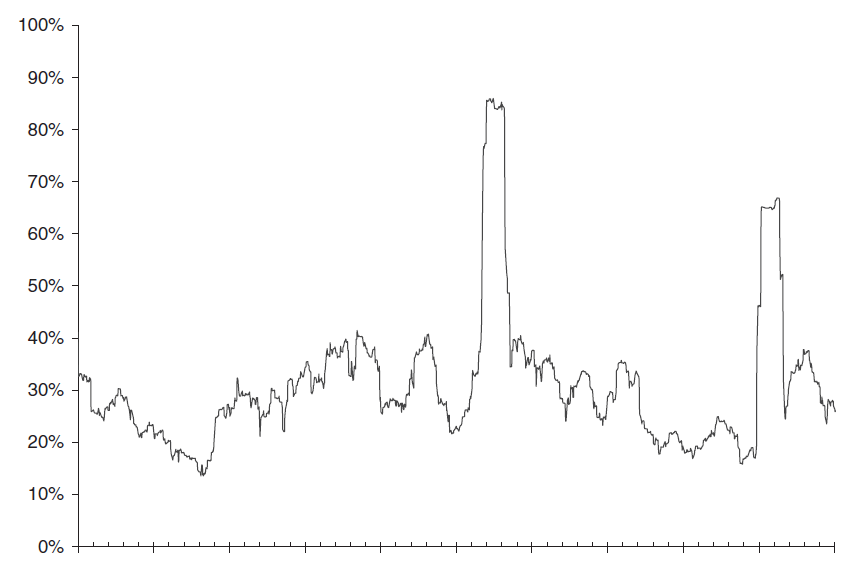
\includegraphics[width=\textwidth]{figure/mw_volatility.png}
        \caption{Moving-window volatility}
    \end{subfigure}
    \begin{subfigure}[b]{0.4\textwidth}
        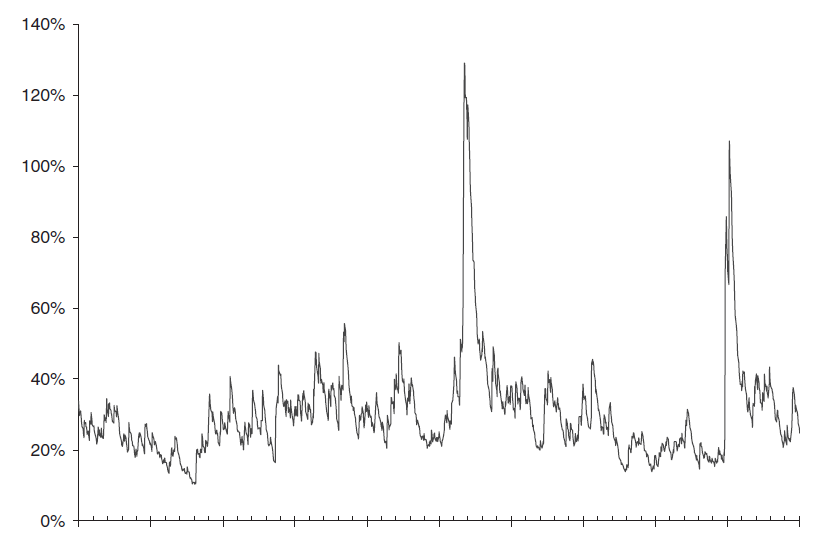
\includegraphics[width=\textwidth]{figure/ew_volatility.png}
        \caption{Exponentially weighted volatility}
    \end{subfigure}
    \caption{Volatility modelling with move-window and exponentially weighted average}
    \label{fig:volatility_modelling_00}
\end{figure}

Figure \ref{fig:volatility_modelling_00} uses the same stock price to estimate the volatility following the moving-window technique and the exponentially-weighted moving average technique. It is clear shown that the first has plateauing whereas the second doesn't have.


\subsubsection{A simple GRACH model}
Put the preceeding models together to get:
\begin{equation}
	\sigma_n^2 = \alpha \bar{\sigma}^2 + (1 - \alpha) \left( \lambda \sigma_{n-1}^2 + (1 - \lambda) R_n^2 \right)
\end{equation}
This is \textbf{GARCH} model, for \textbf{Generalized Autoregressive Conditional Heteroscedasticity}.


\subsubsection{Range-based estimation of volatility}
The problem with estimating volatility is that you need lots and lots of data to avoid sampling-error problems. But then if you use too many days worth of data you will be trying to estimate a parameter during a period when that parameter is almost certainly varying. To avoid this problem, one can use more information contained within a single day which is going down to finer timescales for the data. The problem with that is the behavior of returns over very short timescales, such as minutes, does not appear to be Normally distributed. There is even some evidence that the returns do not have a finite standard deviation. Setting aside such worries, for now. 


\paragraph{Traditional close-to-close measure}
When the drift is small:
\begin{equation}
	\sigma_{cc}^2 = \frac{1}{n} \sum_{i=1}^n \left( \log \left( \frac{C_i}{C_{i-1}} \right) \right)^2
\end{equation}
Here there is a slight change of notation from before; $C_i$ is the closing price on the $i$-th day. To adjust this for the drift take:
\begin{equation}
	\sigma_{cc}^2 = \frac{1}{n-1} \sum_{i=1}^n \left( \left( \log \left( \frac{C_i}{C_{i-1}} \right) \right)^2 - \frac{\left( \log \left( \frac{C_n}{C_0} \right) \right)^2}{n(n-1)} \right)
\end{equation}


\paragraph{Parkinson 1980}
This estimator uses extreme value, the highs $H$ and the lows $L$ during the day:
\begin{equation}
	\sigma_{p}^2 = \frac{1}{4n \log(2)} \sum_{i=1}^n \left( \log \left( \frac{H_i}{L_i} \right) \right)^2
\end{equation}
This is five times more efficient than the close-to-close estimate which means for the same amount of data the variance of the data is one fifth that of the close-to-close measure.


\paragraph{Garman \& Klass 1980}
At 7.4 times more efficient than close-to-close, we have:
\begin{equation}
	\sigma_{gk}^2 = \frac{1}{n} \sum_{i=1}^n \left( 0.511 \left( \log \left( \frac{H_i}{L_i} \right) \right)^2 - 0.019 \log \left( \frac{C_i}{O_i} \right) \log \left( \frac{H_i L_i}{O_i^2} \right) - 2 \log \left( \frac{H_i}{O_i} \right) \log \left( \frac{L_i}{O_i} \right) \right)
\end{equation}
Here $O_i$ is the opening price.


\paragraph{Rogers \& Satchell 1991}
Parkinson and Garman \& Klass are not independent of the drift. Our last simple volatility estimation is:
\begin{equation}
	\sigma_{rs}^2 = \frac{1}{n} \sum_{i=1}^n \left( \log \left( \frac{H_i}{C_i} \right) \log \left( \frac{H_i}{O_i} \right) + \log \left( \frac{L_i}{C_i} \right) \log \left( \frac{L_i}{O_i} \right) \right)
\end{equation}



\section{FDM solutions for Black-Scholes equation (one-factor model)}
\cite{platen_numericalsde_1977, gm_numericalsde_1994, dh_introsde_2001, hg_sdematlab_2006, sm_introsde_2010, mb_numericalsde_2018}

\subsection{Introduction}
Not yet...



\subsection{Differentiation using the grid}
Not yet...



\subsection{Approximating Greeks}
Not yet...



\subsection{Boundary conditions and payoffs}
Not yet...



\subsection{Explicit method}

\subsubsection{Black-Scholes equation}
Not yet...


\subsubsection{Convergence}
Not yet...


\subsubsection{European option}
Not yet...


\subsubsection{American option}
Not yet...


\subsubsection{Runge-Kutta method}
Not yet...


\subsection{Implicit method}

\subsubsection{Crank-Nicolson method}
Not yet...




\section{Binomial model}
\label{sec:binomial_tree}
This section generalizes the numerical illustration of the binomial model for the option value given in Section \ref{sec:intro_binomial_model}. Then, further applications of the binomial model are presented. The content of this section is heavily based on Chapter 3 of \cite{pw_iqf2ed_2007} and Chapter 10 of \cite{pw_mathfinderiv_1995}. It is worth to repeat the Paul Wilmott's comment on the binomial model that ``the binomial model is great for getting intuition about delta hedging and risk-neutral pricing but not for real-life pricing''.


\subsection{Initiation}
In the binomial model, we assume that the asset, which initially has the value $S$, can, during a time step $\delta t$, either:
\begin{itemize}
    \setlength\itemsep{0em}
    \item rise or fall to a value $u \times S$ or $v \times S$, respectively with $0 < v < 1 < u$;
    \item the probability of a rise is $p$ and so the probability of a fall is $1-p$;
    \item the three constants $(u,v,p)$ are chosen to give the binomial walk the same characteristics as the asset we are modeling.
\end{itemize}

For a more proper approach to quantitative finance, instead of using $(u,v,p)$, we write everything in terms of the mean and the standard deviation of the random walk. That involves writing $(u,v,p)$ in terms of what are known as the drift and the volatility of the asset, the drift $\mu$ is the average rate at which the asset rises, and the volatility $\sigma$ is a measure of its randomness. Since we have three parameters to choose $(u,v,p)$ and only two statistical quantities to fit $(\mu,\sigma)$, choices for conversion is unlimited. One of the possible conversion follows:
\begin{align}
    u &= 1 + \sigma \sqrt{\delta t} \\
    v &= 1 - \sigma \sqrt{\delta t} \\
    p &= \frac{1}{2} + \frac{\mu \sqrt{\delta t}}{2 \sigma}    
\end{align}
This conversion will be described in a little bit more details in the next section. The correction of this conversion is, however, examined below.

The expected asset price after one time step is:
\begin{align}
    p u S + (1-p) v S &= \left( \frac{1}{2} + \frac{\mu \sqrt{\delta t}}{2 \sigma} \right) \left( 1 + \sigma \sqrt{\delta t} \right) S + \left( \frac{1}{2} - \frac{\mu \sqrt{\delta t}}{2 \sigma} \right) \left( 1 - \sigma \sqrt{\delta t} \right) \\
                      &= \left( 1 + \mu \delta t \right) S
\end{align}
so the expected change in the asset is $\mu S \delta t$. Because the expected return is $\mu \delta t$ so the expected asset price is corrected.

The variation of change in the asset price is:
\begin{align}
    S^2 &\left( p(u - 1 - \mu \delta t)^2 + (1-p)(v - 1 - \mu \delta t)^2 \right) \\
     &= S^2 \left( \left( \frac{1}{2} + \frac{\mu \sqrt{\delta t}}{2 \sigma} \right) \left( \sigma \sqrt(\delta t) - \mu \delta t \right)^2 + \left( \frac{1}{2} - \frac{\mu \sqrt{\delta t}}{2 \sigma} \right) \left( \sigma \sqrt(\delta t) + \mu \delta t \right)^2 \right) \\
     &= S^2 \left( \sigma^2 \delta t - \mu^2 \delta t^2 \right)
\end{align}
so the standard deviation of asset changes is (approximately) $S \sigma \sqrt{\delta t}$. Because the standard deviation of return is $\sigma \sqrt{\delta t}$ so the standard deviation of asset changes is corrected.

Because of the similarity in the expected change in the asset and the standard deviation of asset changes, it can be concluded that the conversion from $(u,v,p)$ to $(\mu,\sigma)$ is acceptable.



\subsection{Value of an option}
This section is a numerical generalization of Section \ref{sec:intro_binomial_model}. Suppose that we have an underlying asset of value $S$, and we know the value of the option at time $t + \delta t$. Now construct a portfolio at time $t$ consisting of one option and a short position in a quantity $\Delta$ of the underlying. 

At time $t$ this portfolio has value:
\begin{equation}
    \Pi = V - \Delta S
\end{equation}
where the option value $V$ is, for the moment, unknown. At time $t + \delta t$, the option takes one of two values depending on whether the asset rises or falls:
\begin{equation}
    V^+ \quad \text{or} \quad V^-
\end{equation}
and hence, the portfolio becomes either:
\begin{equation}
    V^+ - \Delta u S \quad \text{or} \quad V^- - \Delta u S
\end{equation}
Because we know $V^+, V^-, u, v, S$, the values of both expressions are just linear functions of $\Delta$.



\subsubsection{Hedging}
Having the freedom to choose $\Delta$, we can make the value of this portfolio the same whether the asset rises or falls, i.e. hedging, which means:
\begin{equation}
    V^+ - \Delta u S = V^- - \Delta u S
\end{equation}
by choosing:
\begin{equation}
    \Delta = \frac{V^+ - V^-}{(u-v) \times S}
\end{equation}

The portfolio value is then:
\begin{equation}
    V^+ - \Delta u S = V^+ - \frac{u(V^+ - V^-)}{u-v}
\end{equation}
if the stock rises; or:
\begin{equation}
    V^- - \Delta u S = V^- - \frac{v(V^+ - V^-)}{u-v}
\end{equation}
if the stock falls. And, of course, these two expressions are the same.



\subsubsection{No arbitrage}
Since the value of the portfolio is guaranteed, following the no-arbitrage argument, its value must coincide with the value of the original portfolio plus any interest earned at the risk-free rate. Let's denote the portfolio value by:
\begin{equation}
    \Pi + \delta \Pi
\end{equation}
which just means the original portfolio value plus the change in value. Thus:
\begin{equation}
    \delta \Pi = r \Pi \delta t
\end{equation}

The full formulation for the portfolio value is then:
\begin{equation}
    \Pi + \delta \Pi = \Pi + r \Pi \delta t = \Pi (1 + r \delta t) = V^+ - \frac{u(V^+ - V^-)}{u-v}
\end{equation}
with:
\begin{equation}
    \Pi = V - \Delta S = V - \frac{V^+ - V^-}{u-v}
\end{equation}
Rearrange the above two equations as an equation for $V$ we get:
\begin{equation}
    (1 + r \delta t)V = (1 + r \delta t) \frac{V^+ - V^-}{u-v} + \frac{uV^- - vV^+}{u-v}
\end{equation}
This is an equation for $V$ given $V^+$ and $V^-$ - the option values at the next time step, and the parameters $u$ and $v$ describing the random walk of the asset. 

This equation can also be written in the more compacted form:
\begin{equation}
    V = \frac{1}{1 + r \delta t} \left( p' V^+ + (1-p')V^- \right)
    \label{equ:option_value_binomial}
\end{equation}
in which:
\begin{equation}
    p' = \frac{1}{2} + \frac{r \sqrt{\delta t}}{2 \sigma}
\end{equation}.
The right-hand side of Equation \ref{equ:option_value_binomial} is just like a discounted expectation. The terms in the parentheses are the sum of probabilities multiplied by events. The probability $p'$ is called the \textbf{risk-neutral probability}. It is like the real probability but used in the \textbf{risk-free world}. In the real world, the probability is calculated with the drift $\mu$ instead of the interest rate $r$:
\begin{equation}
    p' = \frac{1}{2} + \frac{r \sqrt{\delta t}}{2 \sigma} \quad \text{vs.} \quad p = \frac{1}{2} + \frac{\mu \sqrt{\delta t}}{2 \sigma} 
\end{equation}. 
Observe that the risk-free interest rate $r$ plays two roles in option valuation. It's used once for discounting to give present value, and it's used as the drift rate in the risk-neutral asset price random walk.

Equation \ref{equ:option_value_binomial} is equivalent to the statement ``the option value at any time is the present value of the risk-neutral expected value at any later time'', so it is actually the risk-neutral expectation.



\subsubsection{Binomial tree}
The binomial tree presents the possible development of the asset value following the random walk of the binomial model all the way until expiry. An example of the binomial tree is given in Figure \ref{fig:binomial_math} where the nodes represent the values taken by the asset. Observe how the tree bends due to the geometric nature of the asset growth although it is normally presented in an equal-distance manner as in Figure \ref{fig:binomial_tree_general}. 

\begin{figure}[H]
    \centering
    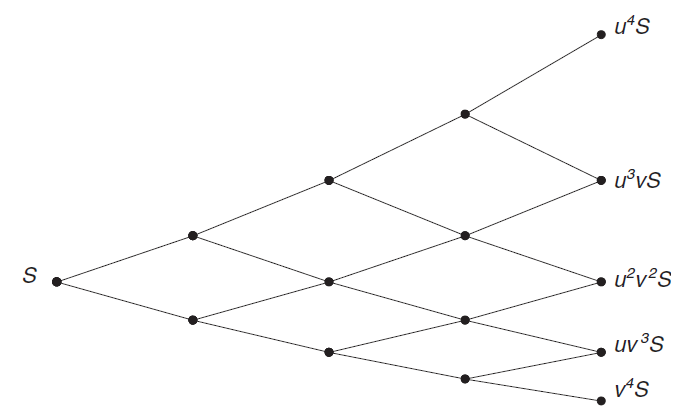
\includegraphics[width=0.6\textwidth]{figure/binomial_math.png}
    \caption{A binomial tree}
    \label{fig:binomial_math}
\end{figure}

The probability of reaching a particular node in the binomial tree depends on the number of distinct paths to that node and the probabilities of the up and down moves. The binomial tree therefore contains within it an approximation to the probability density function for the lognormal random walk, Figure \ref{fig:binomial_tree_general}.

\begin{figure}[H]
    \centering
    \begin{subfigure}[b]{0.4\textwidth}
        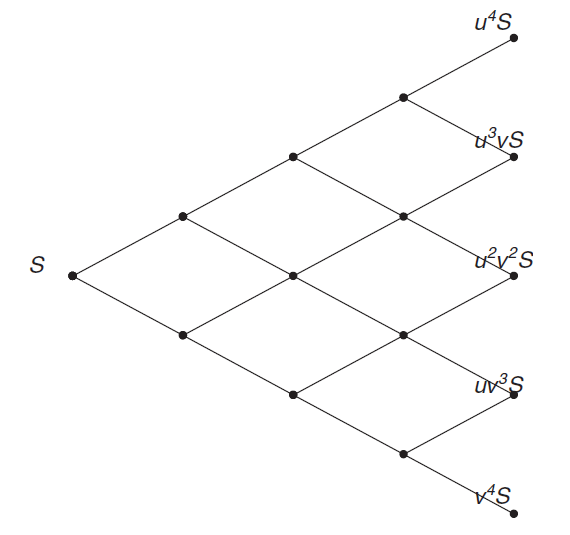
\includegraphics[width=\textwidth]{figure/binomial_schematic.png}
        \caption{Schematic presentation}
    \end{subfigure}
    \begin{subfigure}[b]{0.4\textwidth}
        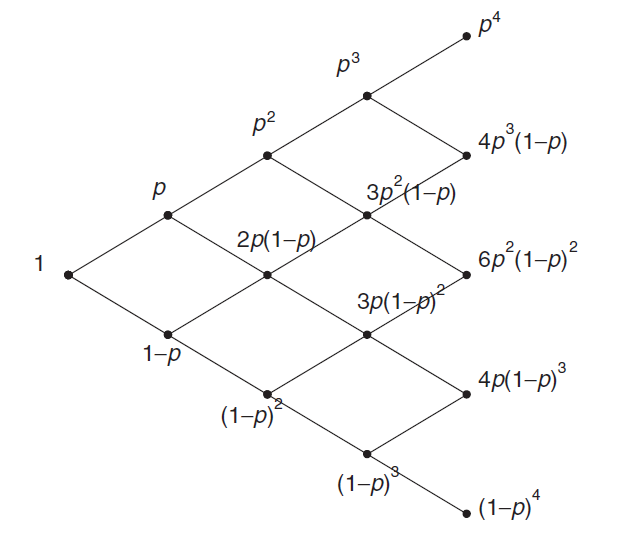
\includegraphics[width=\textwidth]{figure/binomial_counting.png}
        \caption{Counting path - Probability}
    \end{subfigure}
    \caption{A binomial tree}
    \label{fig:binomial_tree_general}
\end{figure}



\subsubsection{The Greeks}
The greeks are defined as derivatives of the option value with respect to various variables and parameters. It is important to distinguish whether the differentiation is with respect to a variable or a parameter. If the differentiation is only with
respect to the asset price and/or time then there is sufficient information in our binomial tree to estimate the derivative. It may not be an accurate estimate, but it will be an estimate. The option's $\Delta$, $\Gamma$ and $\Theta$ can all be estimated from the tree. On the other hand, it is harder if you want to examine the sensitivity of the option with respect to one of the parameters. They are harder to calculate in the sense that you must perform a second binomial calculation. This applies to the option's Vega and $\rho$.

The option's delta is defined by:
\begin{equation}
    \Delta = \frac{V^+ - V^-}{(u-v) \times S}
\end{equation}
As all quantities on the right-hand side are known, we can calculate the delta directly from the tree. In the limit as the time step approaches zero, the delta becomes:
\begin{equation}
    \Delta = \frac{\partial V}{\partial S}
\end{equation}

The gamma of the option is also defined as a derivative of the option with respect to the underlying:
\begin{equation}
    \Gamma = \frac{\partial^2 V}{\partial S^2}
\end{equation}
Gamma is a measure of how much we must rehedge at the next time step. Using the binomial tree, the gamma is just the change in the delta from one of these to the other divided by the distance between them. It, however, will be much easier when we use a finite-difference grid to estimate this quantity.

The theta of the option is the sensitivity of the option price to time, assuming that the asset price does not change. Again, this is easier to calculate from a finite difference grid. An obvious choice for the discrete time definition of theta is to interpolate between $V^+$ and $V^-$ to find a theoretical option value had the asset not changed and use this to estimate:
\begin{equation}
    \Gamma = \frac{\partial V}{\partial t}
\end{equation}
which results in:
\begin{equation}
    \Gamma = \frac{\frac{1}{2} \left( V^+ - V^- \right)}{\delta t}
\end{equation}

Estimating the other type of greeks, the ones involving differentiation with respect to parameters, requires performing a second binomial calculation. The calculation of the option's vega is presented here for illustration. The vega is the sensitivity of the option value to the volatility:
\begin{equation}
    \text{Vega} = \frac{\partial V}{\partial \sigma}
\end{equation}
Suppose we want to find the option value and the vega when the volatility is 20\%. The most efficient way to do this is to calculate the option price twice, using a binomial tree, with two different values of $\sigma$. Calculate the option value using a volatility of $\sigma \pm \varepsilon$, for a small number $\varepsilon$; call the values you find $V_\pm$. The option value is approximated by the average value:
\begin{equation}
    V = \frac{1}{2} \left( V_{+} - V_{-} \right)
\end{equation}
and the vega is approximated by:
\begin{equation}
    \text{Vega} = \frac{V_{+} - V_{-}}{2 \varepsilon}
\end{equation}
The idea can be applied to other greeks.



\subsection{Implementation}
\subsubsection{$(u,v,p)$ to $(\mu,\sigma)$}
The three constants $(u,v,p)$ are chosen to give the binomial walk the same drift and standard deviation $(\mu,\sigma)$ as the stock we are trying to model. Our starting point, the lognormal random walk
\begin{equation}
    dS = \mu \; S \; dt + \sigma \; S \; dX
\end{equation}
has the solution:
\begin{equation}
    S(t) = S(0) e^{\left( \mu - \frac{1}{2} \sigma^2 \right) t + \sigma \phi \sqrt{t}}
\end{equation}
where $\phi$ is a standardized normal random variable. 

For the binomial random walk to have the correct drift over a time period of $\delta t$ we need (details can be found in \cite{pw_mathfinderiv_1995}):
\begin{equation}
    puS + (1-p)vS = S \times E \left[ e^{\left( \mu - \frac{1}{2} \sigma^2 \right) \delta t + \sigma \phi \sqrt{\delta t}} \right] = S \times e^{\mu \delta t}
\end{equation}
i.e.
\begin{equation}
    pu + (1-p)v = e^{\mu \delta t}
\end{equation}
Rearranging this equation gives us:
\begin{equation}
    p = \frac{e^{\mu \delta t} - v}{u - v}
    \label{equ:binomial_cond_1}
\end{equation}

For the binomial random walk to have the correct variance we need (details can be found in \cite{pw_mathfinderiv_1995}):
\begin{equation}
    pu^2 + (1-p)v^2 = e^{\left( 2\mu + \sigma^2 \right)\delta t}
    \label{equ:binomial_cond_2}
\end{equation}

Having only two equations for the three parameters gives us one degree of freedom in this choice. As Equations \ref{equ:binomial_cond_1} and \ref{equ:binomial_cond_2} determine all the statistically important properties of the discrete random walk, the choice of the third equation is somewhat arbitrary. This degree of freedom is often used to give the random walk the further property that after an up and a down movement (or a down followed by an up) the asset returns to its starting value $S$. This gives us the requirement that:
\begin{equation}
    v(uS) = u(vS) = S
\end{equation}
i.e. 
\begin{equation}
	uv = 1
	\label{equ:binomial_cond_3}
\end{equation}
This choice leads to a tree in which the starting asset price reoccurs every even time-step and which is symmetric about this price, Figure \ref{fig:binomial_tree_3rd}(a). Another popular choice is:
\begin{equation}
    p = \frac{1}{2}
\end{equation}
which leads to a tree oriented in the direction of the drift, Figure \ref{fig:binomial_tree_3rd}(b) since the probabilities of an up-jump and a down-jump are equal.

\begin{figure}[H]
    \centering
    \begin{subfigure}[b]{0.45\textwidth}
        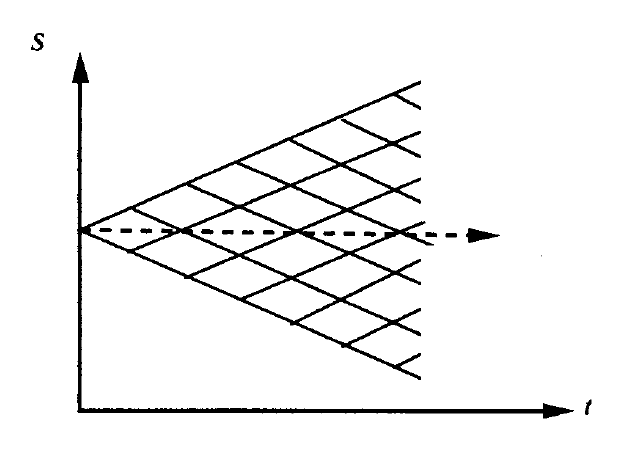
\includegraphics[width=\textwidth]{figure/uv=1.png}
        \caption{A tree with $u \times v = 1$}
    \end{subfigure}
    \begin{subfigure}[b]{0.45\textwidth}
        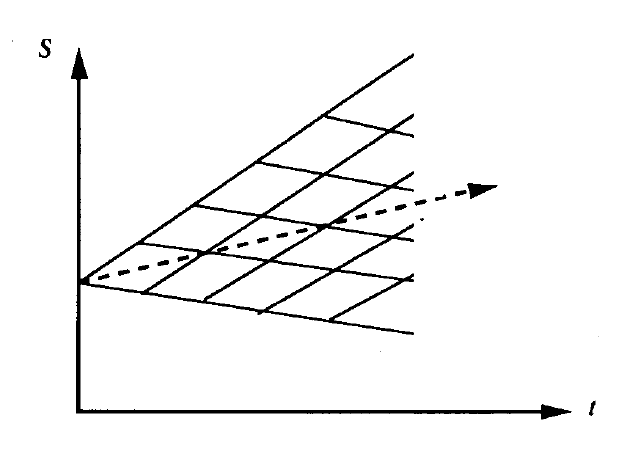
\includegraphics[width=\textwidth]{figure/p=05.png}
        \caption{A tree with $p = \frac{1}{2}$}
    \end{subfigure}
    \caption{Different binomial trees corresponding to the third equation}
    \label{fig:binomial_tree_3rd}
\end{figure}

This note only consider the first choice of freedome; correspondingly, Equations \ref{equ:binomial_cond_1}, \ref{equ:binomial_cond_2} and \ref{equ:binomial_cond_3} can be solved to give:
\begin{equation}
    u = \frac{1}{2} \left( e^{-\mu \delta t} + e^{\left( \mu + \sigma^2 \right)\delta t} \right) + \frac{1}{2} \sqrt{\left( e^{-\mu \delta t} + e^{\left( \mu + \sigma^2 \right)\delta t} \right)^2 - 4}
    \label{equ:binomial_u}
\end{equation}

The following approximations are good enough for most purposes:
\begin{align}
    u &\approx 1 + \sigma \delta t^{1/2} + \frac{1}{2} \sigma^2 \delta t \\
    v &\approx 1 - \sigma \delta t^{1/2} + \frac{1}{2} \sigma^2 \delta t \\
    p &\approx \frac{1}{2} + \frac{\left( \mu - \frac{1}{2} \sigma^2 \right) \delta t^{1/2}}{2 \sigma}
\end{align}

If the above derivation is being used for pricing options, the $\mu$ should be replaced by $r$ everywhere.



\subsubsection{Data structures}
The asset price and the option value are stored in two-dimensional array for clarity. The notation $S_i^n$ means the asset price at the $n$-th time step and at the node $i$ from the bottom, $0 \leq i \leq n$. In the lognormal model:
\begin{equation}
    S_i^n = S \times u^i v^{n-i}
\end{equation}
The notation $V_i^n$ means the option value at the same node. Our goal is to find $V_0^0$ knowing the payoff, i.e. knowing $V_i^N$ for all $0 \leq i \leq N$ where $N$ is the number of time steps. 


\subsubsection{Payoff function}
Assuming that we know the payoff function for our derivative security, and that it depends only on the values of the underlying asset at expiry, we are able to value it at expiry, i.e. time-step $N \delta t$.

If we are considering a put, we find that:
\begin{equation}
    V_i^N = \textbf{max} \left( E - S_i^N, 0 \right) \quad i = 0,1,2...,N
\end{equation}
where $E$ is the exercise price (strike). For a call, we find that:
\begin{equation}
    V_i^N = \textbf{max} \left( S_i^N - E, 0 \right) \quad i = 0,1,2...,N
\end{equation}



\subsubsection{Implementation}
The implementation is quite straight-forward for the European-style exercise. First, we build a tree of possible asset prices; then find the values of the option at expiry using the \textbf{payoff\_function}; finally, calculate the present values of the expected values of the option price under a risk-neutral random walk from expiry back until the present. The algorithm is presented below for the asset price $Asset$, the strike value $E$, the interest rate $r$, the volatility $\sigma$, the expiry $T$ and the number of time step $N$. The code can be found \href{https://github.com/chitn/quantfin_study/blob/master/code/binomial_model.py}{here}. 

\vspace{\baselineskip}
\begin{algorithm}[H]
\caption{European-style exercise}
\label{algo:binomial_european}  
\Begin{
    $Asset, E, r, \sigma, T, N $                      \tcc*[r]{Input} 
    \text{Time step     } $\delta t = \frac{T}{N}$    \tcc*[r]{Initialisation}
    \text{Discount rate } $dcr = \exp(-r \delta t)$                     \\
    \text{Calculate $(u, v, p)$ following \ref{equ:binomial_u}, \ref{equ:binomial_cond_3} and \ref{equ:binomial_cond_1}, respectively} \\
    \text{2D-array of asset value  $S = 0$ and option value $V = 0$}    \\
   
    \tcc*[r]{Calculate asset values}
    \text{Present asset price } $S_0^0 = Asset$  \\
    \For{i = 1 $\rightarrow$ N}{
        $S_0^i = S_0^{i-1} \times v$             \\
        \For{j = i $\rightarrow$ 1}{
            $S_j^i = S_{j-1}^{i-1} \times u$     \\
        }
    }       
    \tcc*[r]{Calculate option values}
    \For{i = 1 $\rightarrow$ N}{                 
         $V_i^N = \textbf{payoff\_function} \left(S_i^N, E\right)$  \\
    } 
    \For{i = N-1 $\rightarrow$ 0}{
        \For{j = 0 $\rightarrow$ i+1}{
            $V_j^i = \left( p \times V_{j+1}^{i+1} + (1-p) \times V_{j}^{i+1} \right) \times dcr$   
        }
    }    
    \text{Present option value } $Option = V_0^0$     
} 
\end{algorithm}
\vspace{\baselineskip}

The implementation for the American-style exercise is almost identical to that for the European-style exercise except a minor modification to address the early exercise to avoid arbitrage, i.e. the option value should be larger or equal to the payoff at any time. If our theoretical value calculated following \ref{equ:option_value_binomial} falls below the payoff then it is time to exercise. 
\begin{equation}
    V_j^i = \textbf{max} \left( \frac{p \times V_{j+1}^{i+1} + (1-p) \times V_{j}^{i+1}}{\exp(r \delta t)},
\textbf{payoff\_function} \left(S_j^i, E\right) \right)
\end{equation}
The algorithm for the American-style exercise is then only different from Algorithm \ref{algo:binomial_european} in calculating the intermediate option values, i.e. the option values is calculated by taking the maximum of the expected values and the payoff for early exercise at each time-step and the asset price.

\vspace{\baselineskip}
\begin{algorithm}[H]
\caption{American-style exercise}
\Begin{
    \For{i = N-1 $\rightarrow$ 0}{
        \For{j = 0 $\rightarrow$ i+1}{
            $\text{Theoretical option value } tv = \left( p \times V_{j+1}^{i+1} + (1-p) \times V_{j}^{i+1} \right) \times dcr $ \\
            $\text{Early exerice value } ev = \textbf{payoff\_function} \left(S_j^i, E\right) $                                  \\
            $V_j^i = \textbf{max} \left( tv, ev \right)$   
        }
    }    
    \text{Present option value } $Option = V_0^0$     
}
\label{algo:binomial_american}   
\end{algorithm}
\vspace{\baselineskip}

Figure \ref{fig:binomial_euam_put} illustrate the option value for European- and American-put options corresponding to different numbers of time steps $N$. The input is as follows $Asset = 100, E = 110, r = 0.06, \sigma = 0.3, T = 0.25 \& 1 \text{ (3-month and 1-year duration)}$.

\begin{figure}[H]
    \centering
    \begin{subfigure}[b]{0.45\textwidth}
        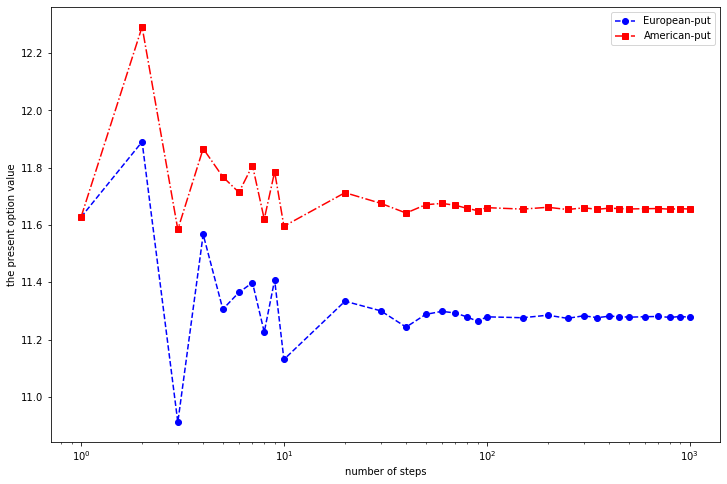
\includegraphics[width=\textwidth]{figure/binomial_model_euam_put_025.png}
        \caption{Expiry in 3-month}
    \end{subfigure}
    \begin{subfigure}[b]{0.45\textwidth}
        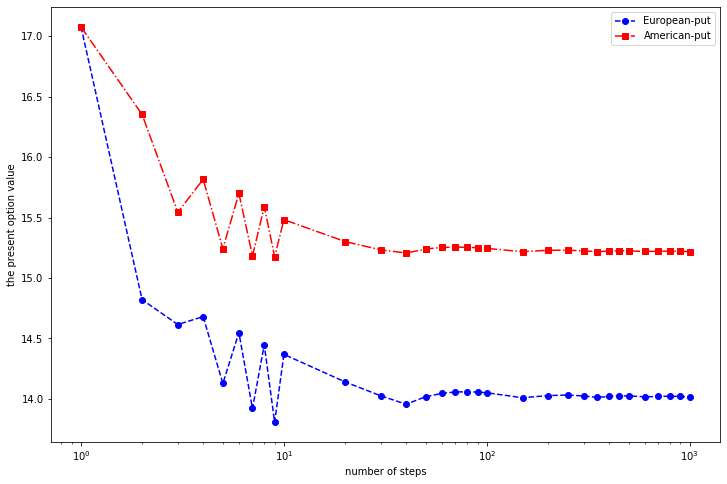
\includegraphics[width=\textwidth]{figure/binomial_model_euam_put_100.png}
        \caption{Expiry in 1-year}
    \end{subfigure}
    \caption{Binomial model for European- and American-put options}
    \label{fig:binomial_euam_put}
\end{figure}



\subsubsection{Dividend yields}
The binomial model can easily accommodate a constant dividend yield $D_0$ paid on the underlying. The effective risk-free growth rate of the asset becomes $\mu - D_0$ instead of $\mu$, that is:
\begin{equation}
    dS = \left( \mu - D_0 \right) \; S \; dt + \sigma \; S \; dX
\end{equation}
therefore we should replace $\mu$ by $\mu - D_0$ in the derivation of $(u,v,p)$. For the case $uv = 1$, the formulations of $(u,v,p)$ become:
\begin{align}
    A &= \frac{1}{2} \left( e^{-\left( \mu - D_0 \right) \delta t} + e^{\left( \mu - D_0 + \sigma^2 \right)\delta t} \right) \\
    u &= A + \sqrt{A^2 - 1} \\
    v &= A - \sqrt{A^2 - 1} \\
    p &= \frac{e^{\left( \mu - D_0 \right) \delta t} - v}{u - v}
\end{align}

The only effect of continuous dividend yields is to modify the probability $p$ and the jump sizes $u$ and $v$. Therefore, the same algorithm given in the previous section for both the European- and American-option values can still be used by simply modifying the parameters $(u,v,p)$ according to the above equations. 


\subsection{Continuous-time limit}
The binomial model is a discrete-time model for the option pricing. From this model, we can develop a continuous-time model (the famous Black-Scholes model) by let $\delta t \rightarrow 0$. 

We will start with the three approximation:
\begin{align*}
    u &\approx 1 + \sigma \sqrt{\delta t} \\
    v &\approx 1 - \sigma \sqrt{\delta t} \\
    p &\approx \frac{1}{2} + \frac{\mu \sqrt{\delta t}}{2 \sigma}    
\end{align*}
as introduced at the beginning of this section.

Next, we write:
\begin{align}
    V   &= V(S , t)                                          \\
    V^+ &= V(uS, t + \delta t) = V(S + (u-1)S, t + \delta t) \\
    V^- &= V(vS, t + \delta t) = V(S + (v-1)S, t + \delta t)   
\end{align}
and apply the Taylor series approximation with small $\delta t$ for $V^+$ and $V^-$ following:
\begin{equation}
    V(S + \delta S, t + \delta t) \approx V(S,t) + \delta t \frac{\partial V}{\partial t} + \delta S \frac{\partial V}{\partial S} + \frac{1}{2} \delta S^2 \frac{\partial^2 V}{\partial S^2} + ...
\end{equation}
This series goes on for ever, but we only use the largest and most important terms, those which are required for the Black–Scholes analysis.

By substituting $V^+$ and $V^-$ into the equation:
\begin{equation*}
    \Delta = \frac{V^+ - V^-}{(u-v) \times S}
\end{equation*}
to achieve:
\begin{equation}
    \Delta \approx \frac{\partial V}{\partial S} \quad \text{as } \delta t \rightarrow 0
\end{equation}

Then, by substituting $V$, $V^+$ and $V^-$ into the equation:
\begin{equation*}
    \left( 1 + r \delta t \right) V = p V^+ + (1-p)V^-
\end{equation*}
to find:
\begin{equation}
    \frac{\partial V}{\partial t} + \frac{1}{2} \sigma^2 S^2 \frac{\partial^2 V}{\partial S^2} + rS \frac{\partial V}{\partial S} - rV = 0
\end{equation}
This is the Black–Scholes equation. Again, the drift rate $\mu$ has disappeared from the equation. 

The famous Black–Scholes equation will be derived later using stochastic calculus rather than via the binomial model. The stochastic calculus derivation is far more useful than the binomial and being far easier to generalize.



\subsection{Miscellaneous \textcolor{red}{[FUTURE]}}
\begin{itemize}
    \setlength\itemsep{0em}
    \item Replicating portfolio
    \item Asset price process
\end{itemize}




\section{Monte-Carlo solution for Geometric Brownian motion}



\section{A trading game}




\chapter{Basic financial simulation II}
\section{Time series analysis}



\section{Statistical techniques}



\section{Machine learning techniques}



\chapter{Basic financial simulation III}
\section{Volatility modelling}
\label{sec:volatility_modelling}
In general, the Black–Scholes model is very robust and does a decent job of pricing derivatives. One of the most important flaws in the model concerns the behavior of volatility. In fact, we do not know what volatility currently is as well as what it may be in the future; whereas the correct pricing of derivatives requires us to know what the volatility is going to be. For this reason, volatility analysis and modeling takes a prominent role in financial simulation.


\subsection{Different types of volatility}
Volatility is difficult to estimate, the best we can hope to do is to measure it statistically. But such a measure is necessarily backwards looking, and we really want to know what volatility is going to be in the future. There are a few types of volatility:
\begin{itemize}
	\setlength\itemsep{0em}
	\item Actual volatility
	\begin{itemize}
		\setlength\itemsep{0em}
		\item This is the measure of the amount of randomness in an asset return at any particular time. It is very difficult to measure, but is supposed to be an input into all option pricing models. In particular, the actual (or `local') volatility goes into the Black–Scholes equation.
		\item There is no `timescale' associated with actual volatility, it is a quantity that exists at each instant, possibly varying from moment to moment.
		\item Example: the actual volatility is now 20\%... now it is 22.5\%...
	\end{itemize}
	\item Historical or realized volatility
	\begin{itemize}
		\setlength\itemsep{0em}
		\item This is a measure of the amount of randomness over some period in the past. The period is always specified, and so is the mathematical method for its calculation. Sometimes this backward-looking measure is used as an estimate for what volatility will be in the future. In pricing an option we are making an estimate of what actual volatility will be over the lifetime of the option. After the option has expired we can go back and calculate what the volatility actually was over the life of the option. This is the realized volatility.
		\item There are two `timescales' associated with historical or realized volatility: one short and one long.
		\item Example: The 60-day volatility using daily returns. Perhaps of interest if you are pricing a 60-day option, which you are hedging daily.
	\end{itemize}
	\item Implied volatility
	\begin{itemize}
		\setlength\itemsep{0em}
		\item The implied volatility is the volatility which when input into the Black–Scholes option pricing formul{\ae} gives the market price of the option. It is often described as the market's view of the future actual volatility over the lifetime of the particular option. However, it is also influenced by other effects such as supply and demand.
		\item There is one `timescale' associated with implied volatility: expiration.
	\end{itemize}
	\item Forward volatility
	\begin{itemize}
		\setlength\itemsep{0em}
		\item The adjective `forward' can be applied to many forms of volatility, and refers to the volatility (whether actual or implied) over some period in the future.
		\item Forward volatility is associated with either a time period, or a future instant.
	\end{itemize}
\end{itemize}



\subsection{To be continued}
\begin{itemize}
	\setlength\itemsep{0em}
	\item Volatility estimation by statistical means
	\item Maximum likelihood estimation
	\item Different approaches to modelling volatility
\end{itemize}



\section{Delta hedging}

\subsection{Classification of hedging strategies}
`Hedging' in its broadest sense means the reduction of risk by exploiting relationships or correlation between various risky investments. The reason for hedging is that it can lead to an improved risk/return. 


\subsubsection{Two main classifications}
Probably the most important distinction between types of hedging is between model-independent and model-dependent hedging strategies.

\paragraph{Model-independent hedging}
An example of such hedging is put-call parity. There is a simple relationship between calls and puts on an asset (when they are both European and with the same strikes and expiries), the underlying stock and a zero-coupon bond with the same maturity. This relationship is completely independent of how the underlying asset changes in value.

\paragraph{Model-dependent hedging}
Most sophisticated finance hedging strategies depend on a model for the underlying asset. The obvious example is the hedging used in the Black–Scholes analysis that leads to a whole theory for the value of derivatives. In pricing derivatives we typically need to at least know the volatility of the underlying asset.


\subsubsection{To be continued}
\begin{itemize}
	\setlength\itemsep{0em}
	\item Delta hedging
	\item Gamma hedging
	\item Vega hedging
	\item Static hedging
	\item Margin hedging
	\item Crash (Platinum) hedging
\end{itemize}



\subsection{To be continued}
\begin{itemize}
	\setlength\itemsep{0em}
	\item Implied versus actual volatilities
	\item Hedge with actual volatility
	\item Hedge with implied volatility
	\item Hedge with different volatilities
	\item Pros and cons of hedging with each volatility
	\item How does implied volatility behave
\end{itemize}



\section{Not yet covered}
\begin{itemize}
    \setlength\itemsep{0em}
    \item Multi-asset options
    \begin{itemize}
		\setlength\itemsep{0em}
		\item Multidimensional lognormal random walk
		\item Measuring correlations
		\item Options of many underlying
		\item And many more
	\end{itemize}
    \item Exotic and path-dependent options
    \item Barrier options
    \item Fixed-income products
    \item Swaps
    \item One-factor interest rate modeling
    \item Interest rate derivatives
\end{itemize}

\chapter{Intermediate financial simulation}
\begin{itemize}
    \setlength\itemsep{0em}
    \item Simulation of portfolio
    \item Simulation of processes with different levels of returns
    \item Simulation of processes with time-varying volatility
    \item Simulation of price processes
    \item Calibrating option pricing models
\end{itemize}
\chapter{Advanced financial simulation}
\begin{itemize}
    \setlength\itemsep{0em}
    \item Portfolio optimization with alternative risk measures
    \item Portfolio optimization with heuristics
    \item Portfolio optimization under Value-At-Risk   
    \item Back-testing 
    \item Back-testing portfolio strategies
    \item Econometric models
\end{itemize}
\chapter{Mathematical tools for finance}

%\section{Probability}

\subsection{Set theory}
Under moving...



\subsection{Permutation and Combination}
Under moving...



\subsection{Probability}
\subsubsection{Basic}
Under moving...


\subsubsection{Conditional probability and Bayes’s formula}
Under moving...



\subsection{Random variables}
\subsubsection{Basis}
Under moving...


\subsubsection{Properties}
Under moving...



\subsection{Discrete random variables}
\subsubsection{Basis}
Under moving...


\subsubsection{Uniform discrete random variable}
Under moving...


\subsubsection{Binomial random variable}
Under moving...


\subsubsection{Geometric random variable}
Under moving...


\subsubsection{Negative binomial random variable}
Under moving...


\subsubsection{Hyper-geometric random variable}
Under moving...


\subsubsection{Poisson random variable}
Under moving...



\subsection{Continuous random variables}
\subsubsection{Basis}
Under moving...


\subsubsection{Expected value}
If $X$ is a continuous random variable having a pdf $f(x)$ then the \textbf{expected value}\index{expected value} of $X$ is given by: 
\begin{equation}
    E[X] = \int_{-\infty}^\infty x f(x) dx
\end{equation}


\subsubsection{Cumulative distribution function (cdf)}
The \textbf{cumulative distribution function}\index{cumulative distribution function}\index{cdf}, $F$, of the random variable $X$ is defined for all real numbers $b$, by:
\begin{equation}
    F(b) = \mathbf{P}\{X \leq b\}
\end{equation}


\subsubsection{Probability density function (pdf)}
We say $X$ admits a \textbf{probability density function}\index{probability density function}\index{pdf} or \textbf{density}\index{density} if:
\begin{equation}
   \mathbf{P}\{X \leq b\} = F(b) = \int_{-\infty}^b f(x) dx 
\end{equation}
for some non-negative function $f$.


\subsubsection{Continuous uniform distribution function}
Under moving...


\subsubsection{Normal random variable}
$X$ is a \textbf{normal random variable}\index{normal random variable} with parameter $\mu$ and $\sigma^2$ if the density of $X$ is given by:
\begin{equation}
    f(x) = \frac{1}{\sqrt{2\pi}\sigma} e^\frac{-(x-\mu)^2}{2\sigma^2} \quad -\infty < x < \infty
\end{equation}
Thus, the cdf of a \textbf{standard random variable}\index{standard random variable}, i.e. one with mean $\mu = 0$ and variance $\sigma^2 = 1$, is given by:
\begin{equation}
    N(x) = \frac{1}{\sqrt{2\pi}} \int_{-\infty}^{0} e^\frac{-y^2}{2} dy
\end{equation}

The random variable $X$ is \textit{log-normally distributed} if for some normally distributed variable $Y$, $X=e^Y$, that is $\ln(X)$ is normally distributed. 


\subsubsection{Exponential random variable}
Under moving...


\subsubsection{Gamma distribution}
Under moving...



\subsection{Relationship between random variables}
\subsubsection{Basis}
Under moving...


\subsubsection{Independent random variables}
Under moving...


\subsubsection{Conditional distribution}
Under moving...


\subsubsection{Joint pdf of functions}
Under moving...


\subsubsection{Expected value of a function}
Under moving...


\subsubsection{Covariance}
Under moving...


\subsubsection{Coefficient of correlation}
Under moving...



\subsection{Miscellaneous}
\subsubsection{Central tendency}
Under moving...


\subsubsection{Moment generating functions}
Under moving...


\subsubsection{Central limit theorem}
Under moving...


\subsubsection{Special series}
Under moving...


%\section{Stochastic processes}
\subsection{Basic}
Under moving...


\subsection{Bernoulli stochastic process}
Under moving...


\subsection{Poisson stochastic process}
Under moving...


\subsection{Discrete-time Markov chains}
\subsubsection{Discrete-time Markov chains}
Not yet...


\subsubsection{Classification of states}
Not yet...


\subsubsection{Steady-state behavior}
Not yet...


\subsubsection{Absorption probabilities and expected time to absorption}
Not yet...


\subsubsection{Random walk models}
Not yet...



\subsection{Continuous-time Markov chains}
\subsubsection{Continuous-time Markov chains}
Not yet...


\subsubsection{Brownian motion}
Not yet...


\subsubsection{Birth-Death process}
Not yet...


%\section{Statistics}
Not yet...


\section{General numerical methods}
\subsection{Polynomial approximation}
A polynomial approximation is an approximation of a curve or a function with a polynomial. In this section we will see how to find a family of polynomials widely used to estimate functions, known as Taylor polynomials or Taylor series.



\subsubsection{Linear and quadratic approximation}
Let's start with approximating a function using its tangent line - a key idea in Euler's method. Assume that we know the function value and its derivative at some point (e.g. $f(a), f'(a)$). We can use these to approximate $f(x)$ for other points $x$ relatively near $a$ by:
\begin{equation}
	f(x) \approx P_1(x) = f(a) + f'(a)(x-a)
\end{equation}
This is called the first order Taylor polynomial of $f(x)$.

To get a better approximation, we can try to use a quadratic polynomial. Another thing we can try is to find a polynomial that has the same value as the function at some point $a$ and the same first and second derivatives there. We can do both by defining the second order Taylor polynomial for $f(x)$ near the point $x = a$ as follows:
\begin{equation}
	f(x) \approx P_2(x) = f(a) + f'(a)(x-a) + \frac{f''(a)}{2}(x-a)^2
\end{equation}



\subsubsection{Higher-order approximation}
By involving more derivatives and getting higher order polynomial we get better and better polynomial approximation. The $n$-th order Taylor polynomial for $x$ near $a$ is given by:
\begin{equation}
	P_n(x) = f(a) + f'(a)(x-a) + \frac{f''(a)}{2}(x-a)^2 + \sum_{i=3}^n \frac{f^{(i}(a)}{i!}(x-a)^i
\end{equation}
As $n$ goes to infinity, we have the \href{https://en.wikipedia.org/wiki/Taylor_series}{Taylor series}. The Taylor series is defined as follows:

\begin{center}
\begin{footnotesize}
\fbox{
\begin{minipage}{0.90\textwidth}

The Taylor series of a real or complex-valued function $f(x)$ that is infinitely differentiable at a real or complex number $a$ is the power series:
\begin{equation}
	P_n(x) = \sum_{n=0}^\infty \frac{f^{(n)}(a)}{n!}(x-a)^n
\end{equation}
where $f^{(n)}(a)$ denotes the $n$-th derivatives of $f$ evaluated at the point $a$. The derivative of order zero of $f$ is defined to be $f$ itself. 

\end{minipage}
}
\end{footnotesize}
\end{center}

Examples of Taylor series for several functions at $a = 0$ are given below:
\begin{itemize}
	\item Single function:
	\begin{itemize}
		\item $e^{x} = \sum_{n=0}^\infty \frac{x^n}{n!} = 1 + x + \frac{x^2}{2} + \frac{x^3}{6} + R_4(x)$
		\item $\ln(1+x) = \sum_{n=0}^\infty (-1)^{n+1} \frac{x^n}{n} = x - \frac{x^2}{2} + \frac{x^3}{3} + R_4(x)$
		\item $\cos(x) = \sum_{n=0}^\infty \frac{(-1)^n}{(2n)!} x^{2n}$
	\end{itemize} 
	\item A function of a function (derivation can be found in Section 14 of \href{https://en.wikipedia.org/wiki/Taylor_series}{this link}:
	\begin{itemize}
		\item $\frac{e^x}{\cos(x)} = 1 + x + x^2 + \frac{2x^3}{3} + \frac{x^4}{2} + R_5(x)$
		\item $\ln(1 + (\cos(x) - 1)) = -\frac{x^2}{2} - \frac{x^4}{12} - \frac{x^6}{45} + R_8(x)$
\end{itemize} 
\end{itemize}
The notation $R_n(x)$ is presented in the next section.



\subsubsection{Residual}
To evaluate how good the approximation is (or how big the error is) we need to calculate the difference between the approximation value and the exact answer. When using the $n$-th order Taylor series $P_n(x)$ centered at $a$ to approximate $f(x)$, the error is:
\begin{equation}
	E = f(x) - P_n(x)
\end{equation}
Often we are only interested in the magnitude of the error $|E|$. Fortunately, there is a simple formula for a bound on the size of the error $|E| = \left| R_n(x) \right|$, the bound is called the residual and is given as:
\begin{equation}
	\left| R_n(x) \right| = \left| \frac{f^{(n+1)}(c)}{(n+1)!}(x-a)^{n+1} \right|
\end{equation}
where $c$ is between $x$ and $a$. Normally, we will chose the value of $c$ in the range $(a;x)$ to maximize the value of $f^{(n+1)}(c)$; or, just choose a value that we know is surely reasonably larger than $f^{(n+1)}(c)$ for all $c \in (a;x)$. 

\begin{center}
\begin{footnotesize}
\fbox{
\begin{minipage}{0.90\textwidth}

\href{http://www.math.smith.edu/~rhaas/m114-00/chp4taylor.pdf}{\textbf{Example}}

Let's consider the magnitude of $R_5(x)$ of function $f = \cos(x)$ at $a = \pi$. We have $f^{(6)(x)} = -\sin(x)$ and $-1 \leq \sin(x) \leq 1$ hence:
\begin{equation}
	\left| f(x) - P_5(x) \right| \leq \left| R_n(x) \right| = \left| \frac{f^{(6)}(c)}{6!}(x-\pi)^6 \right| = \frac{1}{6!}(x-\pi)^6
	\nonumber
\end{equation}

If we approximate $\cos(3)$ by the fifth order Taylor series centered at $\pi$ then we have an error of at most:
\begin{equation}
	\frac{1}{720}(\pi - 3)^6 \approx 1.11 \times 10^{-9}
	\nonumber
\end{equation}

But if we approximate $\cos(1)$ also by the fifth order Taylor series centered at $\pi$ then we have an error of at most:
\begin{equation}
	\frac{1}{720}(\pi - 1)^6 \approx 3.0 \times 10^{-4}
	\nonumber
\end{equation}

\end{minipage}
}
\end{footnotesize}
\end{center}



\subsubsection{Multivariate Taylor series}
The Taylor series may also be generalized to functions of more than one variable as done in Section 19 of \href{https://en.wikipedia.org/wiki/Taylor_series}{this link}. Since the generalized equation is quite lengthy, an example for a two-variable function is given here.

Let's a function $f(x,y)$ depend on two variables $x$ and $y$, then the second order Taylor series at point $(a,b)$ is:
\begin{align}
	f(a,b) &+ (x-a)f_x(a,b) + (y-b)f_y(a,b) \nonumber \\
	       &+ \frac{1}{2!} \left( (x-a)^2 f_{xx}(a,b) + 2(x-a)(y-b) f_{xy}(a,b) + (y-b)^2 f_{yy}(a,b) \right)
\end{align}
where the subscripts denote the respective partial derivatives. A second order Taylor series expansion of a scalar-valued function of more than one variable can be written compactly as:
\begin{equation}
	T(\mathbf{x}) = f(\mathbf{a}) + (\mathbf{x-a})^T D f(\mathbf{a}) + \frac{1}{2!} (\mathbf{x-a})^T \left\{ D^2 f(\mathbf{a}) \right\} (\mathbf{x-a}) 
\end{equation}
where $D f(\mathbf{a})$ is the \href{https://en.wikipedia.org/wiki/Gradient}{gradient} of $f$ evaluated at $\mathbf{x = a}$ and $D^2 f(\mathbf{a})$ is the \href{https://en.wikipedia.org/wiki/Hessian_matrix}{Hessian matrix}. And from these two equations, you can deduce how the higher order Taylor series expansions look like for multivariate functions. 

\begin{center}
\begin{footnotesize}
\fbox{
\begin{minipage}{0.90\textwidth}

\href{http://www.math.smith.edu/~rhaas/m114-00/chp4taylor.pdf}{\textbf{Example}}

Let's practice the Taylor series expansion for a two-variable function $f(x,y) = e^x \ln(1+y)$ centered at $(a,b) = (0,0)$.

First we need to calculate the partial derivatives of $f(x,y)$ and evaluate them at the origin $(a,b)$.
\begin{alignat*}{4}
	& f_x    &&= e^{x} \ln(1+y)             && \quad \rightarrow f_x(0,0)    &&= 0  \\
	& f_y    &&= \frac{e^{x}}{1+y}          && \quad \rightarrow f_y(0,0)    &&= 1  \\
	& f_{xx} &&= e^{x} \ln(1+y)             && \quad \rightarrow f_{xx}(0,0) &&= 0  \\
	& f_{yy} &&= -\frac{e^{x}}{(1+y)^2}     && \quad \rightarrow f_{yy}(0,0) &&= -1 \\	
	& f_{xy} &&= f_{yx} = \frac{e^{x}}{1+y} && \quad \rightarrow f_{xy}(0,0) &&= f_{xy}(0,0) = 1	
\end{alignat*}

Substituting these values in to the general formula to get:
\begin{equation}
	e^{x} \ln(1+y) = T(x,y) = y + xy - \frac{y^2}{2} + ...
	\nonumber
\end{equation}

Now if we assume $(x,y) = (0.2, 0.2)$ and use this formula to approximate $e^{x} \ln(1+y)$ we will have a value of 0.220, the error is $2.69 \times 10^{-3}$.

\end{minipage}
}
\end{footnotesize}
\end{center}



\subsection{Polynomial interpolation}
This section describes the \href{https://en.wikipedia.org/wiki/Lagrange_polynomial}{Lagrange polynomials} which are widely used for polynomial interpolation. For a given set of points $(x_{j},y_{j})$, the Lagrange polynomial is the polynomial of lowest degree that assumes at each value $x_{j}$ there is a corresponding value $y_{j}$, so that the functions coincide at each point.

Given a set of $k+1$ data points:
\begin{equation}
	(x_0,y_0), (x_1,y_1),... ..., (x_k,y_k)
\end{equation}
where no two $x_i$ are the same, the interpolation polynomial in the Lagrange form is a linear combination:
\begin{equation}
	L(x) = \sum_{j=0}^k y_j l_j(x)
\end{equation}
of Lagrange basis polynomials:
\begin{equation}
	l_j(x) = \prod_{o \leq m \leq k} \frac{x - x_m}{x_j - x_m}
\end{equation}
where $0 \leq j \leq k$ and $m \neq j$.

It can be seen that, for all $j \neq i$, we have $l_j(x_i) = 0$ whereas $l_j(x_j) = 1$. It follows that $y_j l_j(x_j) = y_j$ so at each point $x_j$ we have $L(x_j) = y_j$ showing that $L$ interpolates the function exactly.

\begin{center}
\begin{footnotesize}
\fbox{
\begin{minipage}{0.90\textwidth}

\href{https://en.wikipedia.org/wiki/Lagrange_polynomial}{\textbf{Example}}

We wish to interpolate function $y = f(x)$ over the range $1 \leq x \leq 3$ given these three points:
\begin{alignat*}{4}
	& x_0 &&= 1 && \quad \rightarrow f(x_0) &&= 1  \\
	& x_1 &&= 2 && \quad \rightarrow f(x_1) &&= 4  \\
	& x_2 &&= 3 && \quad \rightarrow f(x_2) &&= 9 
\end{alignat*}

The interpolating polynomial is:
\begin{equation}
	L(x) = 1 \times \frac{x-2}{1-2} \frac{x-3}{1-3} + 
	       4 \times \frac{x-1}{2-1} \frac{x-3}{2-3} +
	       9 \times \frac{x-1}{3-1} \frac{x-2}{3-2} = x^2
	\nonumber
\end{equation}

\end{minipage}
}
\end{footnotesize}
\end{center}



\subsection{Numerical integration}
\subsubsection{Definite integrals}
The definite integral of a function $f(x)$ over an interval $[a;b]$ is the limit:
\begin{equation}
	\int_a^b f(x) dx = \lim_{N \rightarrow \infty} \sum_{i=1}^N f(x^*_i) (x_i - x_{i-1}) \quad x^*_i \in [x_{i-1}; x_i]
\end{equation}
and for each $N$:
\begin{equation}
	x_0 = a < x_1 < .. < x_N = b
\end{equation}
is a partition of $[a;b]$ with $N$ subintervals and the values $x^*_i \in [x_{i-1}; x_i]$ chosen in each subintervals is arbitrary. This definition is actually based on a simple idea is that the value of the definite integral represents the net area under the curve of the graph of $y = f(x)$ on the interval $[a;b]$. The term ``net'' means that the areas above and under $x$-axis are positive and negative, respectively. 

Although many integrals can be exactly solved by the \href{https://en.wikipedia.org/wiki/Fundamental_theorem_of_calculus}{fundamental theorem of calculus}, most definite integrals are actually impossible to solve exactly. For example, the famous \href{https://en.wikipedia.org/wiki/Error_function}{error function} in probability:
\begin{equation}
	\text{erf}(x) = \frac{2}{\sqrt{\pi}} \int_0^x e^{-t^2}dt
\end{equation}
is a definite integral which cannot be evaluated in closed form. Because of this reason, numerical integration becomes a good tool in mathematical modelling. The idea of numerical integration comes directly from the definition of integral which is using geometric shapes to approximate the area under the curve $y = f(x)$ to estimate definite integrals. 

In this section, the simplest methods of numerical integration are represented: 
\begin{itemize}
    \setlength\itemsep{0em}
    \item Riemann sums
    \item Newton-Cotes formula
    \item Monte-Carlo integration
\end{itemize}
The implementation of these algorithms can be found \href{https://github.com/chitn/quantfin_study/blob/master/code/integration.py}{here}.



\subsubsection{Riemann sums}
A \href{https://en.wikipedia.org/wiki/Riemann_sum}{Riemann sum} is a certain kind of approximation of an integral by a finite sum. A Riemann sum of a function $f(x)$ over a partition:
\begin{equation}
	x_0 = a < x_1 < x_2 < ... < x_{N-1} < x_N = b
\end{equation}
is defined as a sum of the form:
\begin{equation}
	\sum_{i=1}^N f(x_i^*) (x_i - x_{i-1}) \quad x_i^* \in [x_{i-1}; x_i]
\end{equation}
where each value $x_i^* \in [x_{i-1}; x_i]$ in each subinterval is abitrary. Riemann sums are important because they provide an easy way to approximate a definite integral:
\begin{equation}
	\int_a^b f(x) dx \approx \sum_{i=1}^N f(x_i^*) (x_i - x_{i-1}) \quad x_i^* \in [x_{i-1}; x_i]
\end{equation}
As the product $f(x_i^*) (x_i - x_{i-1})$ is the area of a rectangle of height $f(x_i^*)$ and width $x_i - x_{i-1}$, a Riemann sum can be considered as the area of $N$ rectangles with heights determined by the graph of $y=f(x)$.

The value $x_i^*$ chosen in each subinterval is arbitrary, there are four specific choices giving us different types of Riemann sum:
\begin{itemize}
	\setlength\itemsep{0em}
	\item $x_i^* = x_{i-1}$: left Riemann sum
	\item $x_i^* = x_{i}$: right Riemann sum
	\item $x_i^* = \frac{x_{i-1} + x_i}{2}$: midpoint Riemann sum
	\item trapezoidal sum: technically not a Riemann sum but the average of the left and right Riemann sums
\end{itemize}
Those four methods are usually approached with partitions of equal size. The interval $[a;b]$ is divided into $N$ subintervals, each of length:
\begin{equation}
	\Delta x = \frac{b-a}{N}
\end{equation}
Hence, the points in the partition will be:
\begin{equation}
	a, a + \Delta x, a + 2\Delta x, ..., a + (N-1)\Delta x, b
\end{equation}
\\


\textbf{Left Riemann sum}

Approximating the function by its value at the left-end points we have:
\begin{equation}
	\int_a^b f(x) dx = \left[ f(a) + f(a + \Delta x) + ... + f(b - \Delta x) \right] + \text{Residual}
\end{equation}
The error of this formula will be:
\begin{equation}
	\text{Residual} = \left| \int_a^b f(x) dx - \sum f_\text{left} \right| \leq \frac{M_1(b-a)^2}{2N}
\end{equation}
where $M_1$ is the maximum value of the absolute value of $f'(x)$ on the interval.

\textbf{Right Riemann sum}

Approximating the function by its value at the right-end points we have:
\begin{equation}
	\int_a^b f(x) dx = \left[ f(a + \Delta x) + f(a + 2\Delta x) + ... + f(b) \right] + \text{Residual}
\end{equation}
The error of the right Riemann sum is identical to that of the left Riemann sum.
\\


\textbf{Midpoint Riemann sum}

Approximating the function by its value at the midpoints of intervals we have:
\begin{equation}
	\int_a^b f(x) dx = \left[ f(a + \frac{\Delta x}{2}) + f(a + \frac{3\Delta x}{2}) + ... + f(b - \frac{\Delta x}{2}) \right] + \text{Residual}
\end{equation}
The error of this formula will be:
\begin{equation}
	\text{Residual} = \left| \int_a^b f(x) dx - \sum f_\text{midpoint} \right| \leq \frac{M_2(b-a)^3}{24N^2}
\end{equation}
where $M_2$ is the maximum value of the absolute value of $f^{(2)}(x)$ on the interval.
\\


\textbf{Trapezoidal sum}

In this case, the values of the function $f(x)$ on an interval are approximated by the values at the left- and right-end points, i.e. the area of the trapezoid formed by these two points. Following the same approach above we have:
\begin{equation}
	\int_a^b f(x) dx = \frac{1}{2} \Delta x \left[ f(a) + 2f(a + \Delta x) + 2f(a + 2\Delta x) + ... 2f(b - \Delta x) + f(b) \right] + \text{Residual}
\end{equation}
The error of this formula will be:
\begin{equation}
	\text{Residual} = \left| \int_a^b f(x) dx - \sum f_\text{midpoint} \right| \leq \frac{M_2(b-a)^3}{12N^2}
\end{equation}
\\


\textbf{Higher dimensions}

In two dimensions, the domain $A$ can be divided into a number of cells $A_i$ and each cell can be interpreted as having an ``area'' denoted by $\Delta A_i$. The Riemann sum is then:
\begin{equation}
	S = \sum_{i=1}^N f(x_i^*, y_i^*) \Delta A_i
\end{equation}
where $(x_i^*,y_i^*) \in A_i$.

Similarly, the domain $V$ in three dimensions can be divided into a number of cells $V_i$ and each cell can be interpreted as having a ``volume'' denoted by $\Delta V_i$. The Riemann sum is then:
\begin{equation}
	S = \sum_{i=1}^N f(x_i^*, y_i^*, z_i^*) \Delta V_i
\end{equation}
where $(x_i^*,y_i^*,z_i^*) \in V_i$. 

Figure \ref{fig:Riemann_sum} presents the Riemann sum of an integral:
\begin{equation}
	\int_0^5 x^{\sin(x)} + x^{\cos(x)} - \sqrt{x} dx
\end{equation}
with a small number of interval, $N = 30$, to illustrate the approximation. This example can be found \href{https://github.com/chitn/quantfin_study/blob/master/code/integration.py}{here}.

\begin{figure}[H]
    \centering
    \begin{subfigure}[b]{0.45\textwidth}
        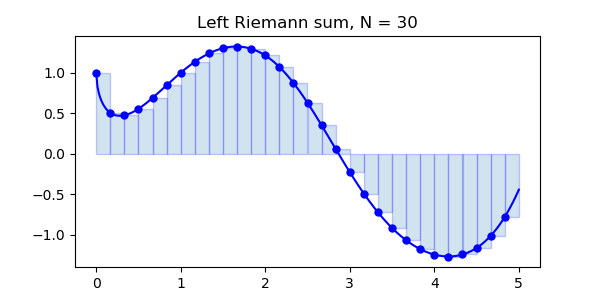
\includegraphics[width=\textwidth]{figure/riemann_left.png}
        \caption{Left Riemann sum}
    \end{subfigure}
    \begin{subfigure}[b]{0.45\textwidth}
        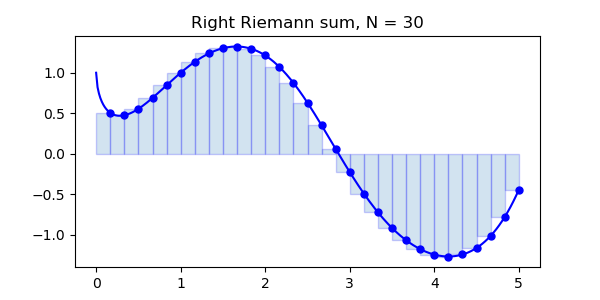
\includegraphics[width=\textwidth]{figure/riemann_right.png}
        \caption{Right Riemann sum}
    \end{subfigure}
    \begin{subfigure}[b]{0.45\textwidth}
        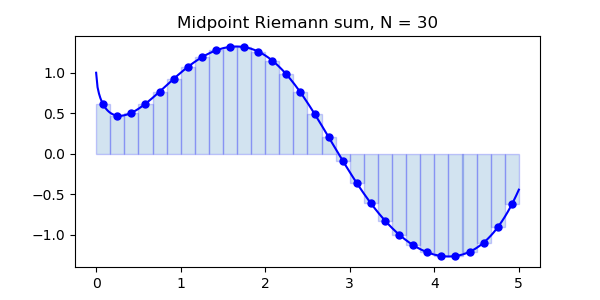
\includegraphics[width=\textwidth]{figure/riemann_mid.png}
        \caption{Midpoint Riemann sum}
    \end{subfigure}
    \begin{subfigure}[b]{0.45\textwidth}
        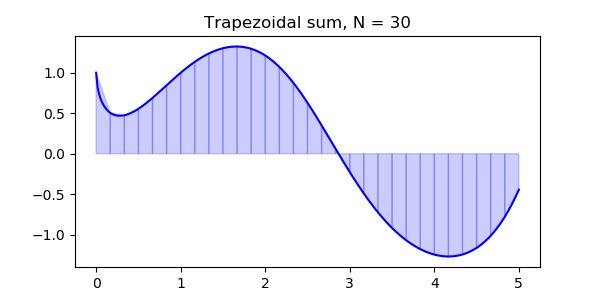
\includegraphics[width=\textwidth]{figure/riemann_trap.png}
        \caption{Trapezoidal sum}
    \end{subfigure}
    \caption{Riemann integration}
    \label{fig:Riemann_sum}
\end{figure}



\subsubsection{Newton-Cotes formulas}
\href{https://en.wikipedia.org/wiki/Newton-Cotes_formulas}{Newton–Cotes formulas}, also called the Newton–Cotes (quadrature) rules, are a group of formulas for numerical integration (also called quadrature) based on evaluating the integral at equally spaced points. If it is required that the points at which the integral is evaluated are not equally spaced, then other methods such as Gaussian quadrature are probably more suitable.

It is assumed that the value of a function $f$ defined on $[a;b]$ is known at equally spaced points $x_i$, for $i = 0, ..., n$, where $x_0 = a$ and $x_n = b$. There are two types of Newton–Cotes formulas, the ``closed'' type which uses the function value at all points, and the ``open'' type which does not use the function values at the endpoints. The Newton–Cotes formulas of degree $n$ are stated as:
\begin{align}
	\int_a^b f(x) dx &\approx \sum_{i=0}^{n} w_i f(x_i)   \quad \text{``close''} \\
	\int_a^b f(x) dx &\approx \sum_{i=1}^{n-1} w_i f(x_i) \quad \text{``open''}
\end{align}
where $x_i = ih + x_0$ with $h = \frac{x_n - x_0}{b} = \frac{b - a}{n}$ is called the step size. The $w_i$ are called weights and are derived from the Lagrange basis polynomials. They depend only on the $x_i$ and not on the function $f$. Let $L(x)$ be the interpolation polynomial in the Lagrange form for the given data points $(x_0, f(x_0)), ..., (x_n, f(x_n))$, then:
\begin{equation}
	\int_a^b f(x) dx \approx \int_a^b L(x) dx = \int_a^b \left( \sum_{i=0}^n f(x_i) l_i(x) \right) dx = \sum_{i=0}^n f(x_i) \underbrace{\int_a^b l_i(x) dx}_{w_i}
\end{equation}

The Newton-Cotes formulas, in fact, cover some other rules such as Riemann midpoint, trapezoidal sum, Simpson's rule... The following table lists some of the Newton-Cotes formulas (the notation $f_i$ is the shorthand for $f(x_i) = f(a + i \frac{b-a}{n}$):
\begin{table}[H]
\begin{center}
\caption{Numerical integration with Newton-Cotes formulas}
\begin{tabular}{cclll}
\multicolumn{5}{c}{Closed Newton-Cotes formulas}                                                                              \\
Degree $n$ & Step size $h$   & Common name       & Formula                                 & Error bound                      \\
\hline
1          & $b-a$           & Trapezoid rule    & $\frac{h}{2} (f_0 + f_1)$               & $\frac{1}{12} h^3 f^{(2)}(\xi)$  \\
2          & $\frac{b-a}{2}$ & Simpson's rule    & $\frac{h}{3} (f_0 + 4f_1 + f_2)$        & $\frac{1}{90} h^5 f^{(4)}(\xi)$  \\
3          & $\frac{b-a}{3}$ & Simpson's 38 rule & $\frac{3h}{8} (f_0 + 3f_1 + 3f_2 + f_3)$ & $\frac{3}{80} h^5 f^{(4)}(\xi)$  \\
           &                 &                   &                                         &                                  \\
\multicolumn{5}{c}{Open Newton-Cotes formulas}                                                                                \\
Degree $n$ & Step size $h$   & Common name       & Formula                                 & Error bound                      \\
\hline
2          & $\frac{b-a}{2}$ & Midpoint rule     & $2h f_1$                                & $\frac{1}{3} h^3 f^{(2)}(\xi)$   \\
3          & $\frac{b-a}{3}$ & Trapezoid rule    & $\frac{3h}{2} (f_1 + f_2)$              & $\frac{1}{4} h^3 f^{(2)}(\xi)$   \\
4          & $\frac{b-a}{4}$ & Milne's rule      & $\frac{4h}{3} (2f_1 - f_2 + 2f_3)$      & $\frac{28}{90} h^5 f^{(4)}(\xi)$
\end{tabular}
\end{center}
\end{table}



\subsubsection{Monte-Carlo integration}
Monte-Carlo integration uses random sampling of a function to numerically compute an estimate of its integral. Suppose that we want to integrate the one-dimensional function $f(x)$ from $a$ to $b$:
\begin{equation}
	F = \int_a^b f(x) dx
\end{equation}
We can approximate this integral by averaging samples of the function $f$ at uniform random points within the interval. Given a set of $N$ uniform random variables $X_i \in [a;b)$ with a corresponding PDF of $\frac{1}{b-a}$, the Monte Carlo estimator for computing $F$ is:
\begin{equation}
	\langle F^N \rangle = (b-a) \frac{1}{N-1} \sum_{i=0}^N f(X_i)
\end{equation}
The random variable $X_i \in [a;b)$ can be constructed by warping a random number uniformly distributed between zero and one, $\xi \in [0;1)$:
\begin{equation}
	X_i = a + \xi (b-a)
\end{equation}
Using this construction, we can expand the estimator to:
\begin{equation}
	\langle F^N \rangle = (b-a) \frac{1}{N} \sum_{i=0}^{N-1} f(a + \xi (b-a))
\end{equation}
Sine $\langle F^N \rangle$ is a function of $X_i$, it is also a random variable; and therefore, $\langle F^N \rangle$ is an approximation of $F$ using $N$ samples.

It is possible to show that:
\begin{equation}
	E \left[ \langle F^N \rangle \right] = F \quad \text{note that } pdf(F) = \frac{1}{b-a}
\end{equation}
As we increase the number of samples $N$, the estimator $\langle F^N \rangle$ becomes closer approximation of $F$. Due to the \textit{Law of Large Numbers}, in the limit we can guarantee that we have the exact solution:
\begin{equation}
	Pr \left\{ \lim_{N \rightarrow \infty} \langle F^N \rangle = F \right\} = 1
\end{equation}
We can estimate convergence of this estimation by determining the convergence rate of the estimators variance. It is possible to show that:
\begin{equation}
	\sigma \left[ \langle F^N \rangle \right] \propto \frac{1}{\sqrt{N}}
\end{equation}
This means that we must quadruple the number of samples in order to reduce the error by half. Standard integration techniques exist which converge much faster in one dimension, that's why Monte-Carlo integration is not a preference in one-dimensional problem. However the convergence rate of basic techniques becomes exponentially worse with increased dimensions; whereas the basic Monte Carlo estimator above can easily be extended to multiple dimensions, Algorithm \ref{algo:mc_inte}, and the convergence rate for Monte Carlo is independent of the number of dimensions in the integral. This makes Monte Carlo integration the only practical technique for many high dimensional integration problems. More details information on the Monte-Carlo integration can be found \href{https://cs.dartmouth.edu/~wjarosz/publications/dissertation/appendixA.pdf}{here} and \href{https://en.wikipedia.org/wiki/Monte_Carlo_integration}{here}.

\vspace{\baselineskip}
\begin{algorithm}[H]
\caption{Monte-Carlo integration}
\label{algo:mc_inte}  
\Begin{
    $x_{\min}, x_{\max}, y_{\min}, y_{\max}$  \tcc*[r]{Input} 
    Function $f(x,y)$, Number of sample $N$   \\
    Set temporary variable $tmp = 0$          \tcc*[r]{Initialisation}
    \For{$i = 1 \rightarrow N$}{
    	$x = \text{random.uniform} \in [x_{\min}; x_{\max}]$   \\
    	$y = \text{random.uniform} \in [y_{\min}; y_{\max}]$   \\
    	$tmp \mkern9mu +\!= f(x,y)$
	}
	$estimator = (x_{\max} - x_{\min}) (y_{\max} - y_{\min}) \frac{tmp}{N}$
} 
\end{algorithm}
\vspace{\baselineskip}

Another way of implementing the Monte-Carlo integration, following closely a counting-approach and geometrical definition of the integral can be found in Algorithm \ref{algo:mc_inte_1d}. This algorithm is, however, harder to generalize into multiple dimensions. 

\vspace{\baselineskip}
\begin{algorithm}[H]
\caption{Monte-Carlo integration by geometrical counting}
\label{algo:mc_inte_1d}  
\Begin{
    $x_{\min}, x_{\max}$                                        \tcc*[r]{Input} 
    Function $f(x)$, Number of sample $N$                       \\
    Finding bounds of $f(x) = f_{\min}, f_{\max}$               \tcc*[r]{Initialisation}
    Set counting variable $count = 0$, indicator vector $z$ (can be zero-initialized here) \\
    \For{$i = 1 \rightarrow N$}{
    	$x  = \text{random.uniform} \in [x_{\min}; x_{\max}]$   \\
    	$fx = f(x)$                                             \\
    	$ft = \text{random.uniform} \in [f_{\min}; f_{\max}]$   \\
    	\uIf{$|ft| \leq |fx|$}{
    		\If{$ft > 0$ \text{and} $fx > 0$ \text{and} $ft < fx$}{
    			$count \mkern9mu +\!= 1$               \tcc*[r]{area over x-axis is positive}
    			$\mathbf{z}[i] = 1$
    		}
    		\If{$ft < 0$ \text{and} $fx < 0$ \text{and} $ft \geq fx$}{
    			$count \mkern9mu -\!= 1$               \tcc*[r]{area under x-axis is negative}  
    			$\mathbf{z}[i] = -1$
    		}
    	}
    	\Else{
    		$\mathbf{z}[i] = 0$
    	}
	}
	$estimator = (x_{\max} - x_{\min}) (y_{\max} - y_{\min}) \frac{count}{N}$  \\
	Plotting with the indicator vector $\mathbf{z}$
} 
\end{algorithm}
\vspace{\baselineskip}

Figure \ref{fig:mc_inte_1d} presents the Monte-Carlo integration following Algorithm \ref{algo:mc_inte_1d} for an integral:
\begin{equation}
	\int_{10}^{20} x^2 \sin(x)^3 dx
\end{equation}
The results for a sample of 100.000 sample points following Algorithm \ref{algo:mc_inte} and \ref{algo:mc_inte_1d} are -181.04 and -182.12, respectively. The results from \href{https://www.wolframalpha.com/input/?i=integrate+x^2+sin^3+x+dx+from+10+to+20}{WolframAlpha} is -181.16. The approximation of this integral by the Riemann sum with 10.000 interval yields the result of -181.16. This example can be found \href{https://github.com/chitn/quantfin_study/blob/master/code/integration.py}{here}.

\begin{figure}[H]
    \centering
    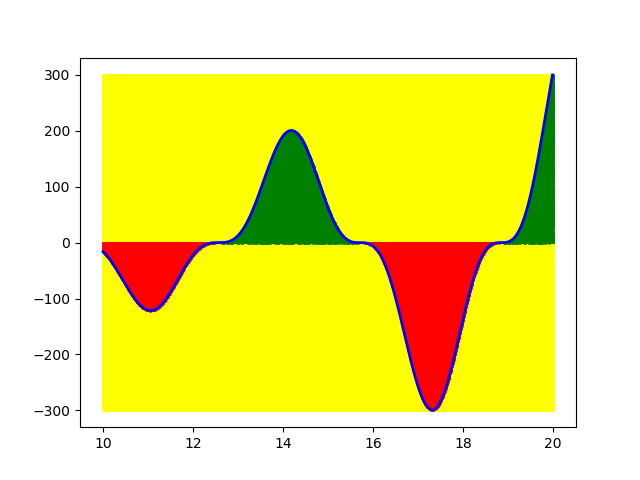
\includegraphics[width=0.75\textwidth]{figure/monte_carlo_inte.png}
    \caption{Monte-Carlo integration}
    \label{fig:mc_inte_1d}
\end{figure}



\subsection{Numerical differentiation}

\subsubsection{Derivative and differentiation}
The \href{https://en.wikipedia.org/wiki/Derivative}{derivative} of a function of a real variable measures the sensitivity to change of the function value (output value) with respect to a change in its argument (input value). Differentiation is the action of computing a derivative. The derivative of a function $y = f(x)$ of a variable $x$ is a measure of the rate at which the value $y$ of the function changes with respect to the change of the variable $x$. By definition we have:
\begin{equation}
	f'(a) = \lim_{h \rightarrow 0} \frac{f(a+h) - f(a)}{h}
\end{equation}
When the limit exists, $f$ is said to be differentiable at $a$. The derivative satisfies the property that:
\begin{equation}
	\lim_{h \rightarrow 0} \frac{f(a+h) - (f(a) + f'(a) \times h)}{h} = 0
\end{equation}
which means:
\begin{equation}
	f(a+h) \approx f(a) + f'(a) h
\end{equation}
for $f$ near $a$. This interpretation can be extended further easily. For example, if $f$ is twice differentiable then:
\begin{equation}
	f(a+h) \approx f(a) + f'(a) h + \frac{1}{2} f''(a) h^2
\end{equation}
If $f$ is infinitely differentiable, then this is the beginning of the Taylor series for $f$ evaluated at $a+h$ around $a$. Consequently, the simplest method to estimate the derivatives to an arbitrary order of accuracy is to use \href{https://en.wikipedia.org/wiki/Numerical_differentiation}{finite difference approximations} which can be central, forward or backward.



\subsubsection{First derivative}
Following the finite difference approximations, the first derivative is calculated as follows:
\begin{itemize}
	\setlength\itemsep{0em}
	\item The forward difference formula with step size $h$
	\begin{equation}
		f'(a) \approx \frac{f(a+h) - f(a)}{h}
	\end{equation}
	\item The backward difference formula
	\begin{equation}
		f'(a) \approx \frac{f(a) - f(a-h)}{h}
	\end{equation}
	\item The central difference formula is the average of the forward and backwards difference formulas
	\begin{equation}
		f'(a) \approx \frac{f(a+h) - f(a-h)}{2h}
	\end{equation}
\end{itemize}
It can be seen that the finite difference approximations are based on the Taylor series, therefore the error in the finite difference approximations can be derived from Taylor's theorem:
\begin{itemize}
	\setlength\itemsep{0em}
	\item The error of the forward difference formula
	\begin{equation}
		\left| \frac{f(a+h) - f(a)}{h} - f'(a) \right| \leq \frac{h F}{2}
	\end{equation}
	with $|f''(x)| \leq F$ for all $x in [a;a+h]$. This error formula is hold for the backward difference formula as well.
	\item The error of the central difference formula
	\begin{equation}
		\left| \frac{f(a+h) - f(a-h)}{2h} - f'(a) \right| \leq \frac{h^2 C}{6}
	\end{equation}
	with $|f'''(x)| \leq C$ for all $x in [a-h;a+h]$.
\end{itemize}
An important consideration in practice when the function is calculated using floating-point arithmetic is the choice of step size $h$. If $h$ is too small, the subtraction will yield a large rounding error due to cancellation. If $h$ is too large, apparently, the accuracy reduces. For the numerical derivative formula evaluated at $x$ and $x + h$, a choice for $h$ that is large enough to avoid the large rounding error of $\sqrt{\varepsilon}x$, where the machine epsilon $\varepsilon = 2.2 \times 10^{-16}$ but small enough to avoid the secant error for optimum accuracy; such an option can be:
\begin{equation}
	h = \sqrt{\varepsilon \left| \frac{f(x)}{f''(x)} \right|}
\end{equation}

In the family of the finite difference approximations, you can achieve approximation with higher order of accuracy by involving more terms of the Taylor series or \href{https://en.wikipedia.org/wiki/Finite_difference_coefficient}{finite difference coefficient}.



\subsubsection{Higher derivative}
Approximations of higher derivatives $f''(x), f'''(x),...$ can easily be obtained in by using the Talor series expansion as above. For example, the central difference formula for the second derivative is as follows:
\begin{align}
	f(a+h) &= f(a) + hf'(a) + h^2\frac{f''(a)}{2!} + h^3\frac{f'''(a)}{3!} + h^4\frac{f^{(4)}(\xi_+)}{4!} ... \nonumber \\
	f(a-h) &= f(a) - hf'(a) + h^2\frac{f''(a)}{2!} - h^3\frac{f'''(a)}{3!} + h^4\frac{f^{(4)}(\xi_-)}{4!} ... \nonumber \\
	\rightarrow f(a+h) + f(a-h) &= 2f(a) + h^2f''(a) + h^4 \frac{f^{(4)}(\xi_+) + f^{(4)}(\xi_-)}{24} \nonumber \\
	\rightarrow f''(a) &\approx \frac{f(a+h) - 2f(a) + f(a-h)}{h^2}
\end{align}
and the error term is:
\begin{equation}
	h^2 \frac{f^{(4)}(\xi_+) + f^{(4)}(\xi_-)}{24}
\end{equation}
in which $\xi_{+/-}$ is a small number between $a$ and $a+h$.

Other forms with the same or higher order of accuracy of finite difference formulas can be found \href{https://en.wikipedia.org/wiki/Finite_difference_coefficient}{here}.



\subsubsection{Partial derivatives}
Given a function of multiple variables, differentiation generalises in a simple way: differentiating the resulting function as a function of one variable while keeping other variable fixed. Finite difference formulas for partial derivatives follows the same approach. For example, the central difference formulas for a function of two variables are as follows:
\begin{align}
	\frac{\partial f}{\partial x}(a,b) &\approx \frac{f(a+h,b) - f(a-h,b)}{2h}  \\
	\frac{\partial f}{\partial y}(a,b) &\approx \frac{f(a,b+k) - f(a,b-k)}{2k}  \\
	\frac{\partial^2 f}{\partial x^2}(a,b) &\approx \frac{f(a+h,b) - 2f(a,b) + f(a-h,b)}{h^2}  \\
	\frac{\partial^2 f}{\partial x \partial y}(a,b) &\approx \frac{f(a+h,b+k) - f(a+h,b-k) - f(a-h,b+k) + f(a-h,b-k)}{4hk} 	
\end{align}    
Sometimes, the notation:
\begin{alignat*}{4}
	& f(a+h,b+k) &&= f_{1,1}  && \quad f(a+h,b-k) &&= f_{1,-1}  \\
	& f(a-h,b+k) &&= f_{-1,1} && \quad f(a-h,b-k) &&= f_{-1,-1} 
\end{alignat*}
is used in \href{https://www.uio.no/studier/emner/matnat/math/MAT-INF1100/h07/undervisningsmateriale/kap7.pdf}{practice}, then the finite difference formula for partial derivatives can be shortened, for example:
\begin{equation}
	\frac{\partial^3 f}{\partial x^2 \partial y} \approx \frac{f_{2,1} - 2f_{0,1} + f_{-2,1} - f_{2,-1} + f_{0,-1} - f_{-2,-1}}{8h^2k}
\end{equation}

\begin{center}
\begin{footnotesize}
\fbox{
\begin{minipage}{0.90\textwidth}

\href{http://www.ohiouniversityfaculty.com/youngt/IntNumMeth/lecture27.pdf}{\textbf{Example}}

Suppose $u = u(x,y)$ is a function of two variables that we only know at grid points $(x_i, y_j)$. The values of $u$ at $(x_i, y_j)$ are recorded in the matrix:
\begin{equation*}
	u(x_i, y_j) = 
	\begin{pmatrix}
		5.1 & 6.5 & 7.5 & 8.1 & 8.4  \\
		5.5 & 6.8 & 7.8 & 8.3 & 8.9  \\
		5.5 & 6.9 & 9.0 & 8.4 & 9.1  \\
		5.4 & 9.6 & 9.1 & 8.6 & 9.4
	\end{pmatrix}
\end{equation*}
Suppose that the grid points are evenly spaced in both $x-$ and $y-$direction with $h = 0.5$ and $k = 0.2$. Then $u_y(x_2, y_4)$ can be approximated by the central difference as follows:
\begin{equation*}
	u_y(x_2, y_4) \approx \frac{u_{2,5} - u_{2,3}}{2k} \approx \frac{8.9 - 7.8}{2 \times 0.2} = 2.75
\end{equation*}

Similarly, $u_{xy}(x_2, y_4)$ can be approximated as:
\begin{equation*}
	u_{xy}(x_2, y_4) \approx \frac{u_{3,5} - u_{3,3} - u_{1,5} + u_{1,3}}{4hk} \approx \frac{9.1 - 9.0 -8.4 + 7.5}{4 \times 0.2 \times 0.5} = -2.0
\end{equation*}

\end{minipage}
}
\end{footnotesize}
\end{center}

Figure \ref{fig:nume_deriv} presents the first and second derivative of a function calculated by the numerical differentiation with the finite difference approach. The implementation can be found \href{https://github.com/chitn/quantfin_study/blob/master/code/differentiation.py}{here}.

\begin{figure}[H]
    \centering
    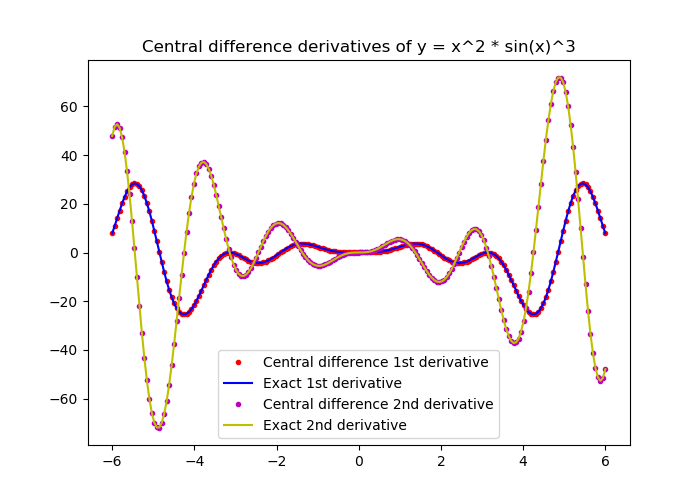
\includegraphics[width=0.75\textwidth]{figure/derivative.png}
    \caption{First and second derivatives calculated with numerical differentiation}
    \label{fig:nume_deriv}
\end{figure}



\subsection{Root finding}
In mathematics and computing, a \href{https://en.wikipedia.org/wiki/Root-finding_algorithms}{root-finding algorithm} is an algorithm for finding zeroes of continuous functions, i.e. a number/vector $x$ for which $f(x) = 0$. Generally, the zeroes of a function cannot be computed exactly nor expressed in closed form, root-finding algorithms provide approximations to those. There are many algorithms for finding roots, this section only describes three basic algorithms, namely:
\begin{itemize}
	\setlength\itemsep{0em}
	\item Bisection method
	\item Newton-Raphson method
	\item Secant method
\end{itemize}
The implementation of these algorithms can be found \href{https://github.com/chitn/quantfin_study/blob/master/root_finding.py}{here}.



\subsubsection{Bisection method}
The simplest root-finding algorithm is the \href{https://en.wikipedia.org/wiki/Bisection_method}{bisection method} which can apply to any continuous function $f(x)$ on an interval $[a;b]$ where the value of the function $fx)$ changes sign from $a$ to $b$, i.e. $f(a) \times f(b) < 0$. The idea is simple: divide the interval in two, a solution must exist within one sub-interval, select the sub-interval where the sign of $f(x)$ changes and repeat until the root is found. Following this algorithm, we can easily estimate the absolute error of the approximation after $N$ iteration as:
\begin{equation}
	\left| x_{\text{exact}} - x_N \right| \leq \frac{b - a}{2^{N+1}}
\end{equation}
From this equation, we can also calculate the minimum number of iteration required to achieve the absolute error less than a certain threshold $\epsilon$ as follows:
\begin{equation}
	N \geq \frac{\log{\frac{b-a}{\epsilon}}}{\log(2)} - 1
\end{equation}
Although Bisection method is easy to implement and quite robust, generalization of Bisection method to a multivariate problem is not straightforward. 



\subsubsection{Newton-Raphson method}
\href{https://en.wikipedia.org/wiki/Newton's_method}{Newton–Raphson method} is a root-finding algorithm which produces successively better approximations to the roots of a real-valued function.  
\\


\textbf{Single-variable function}

Given a single-variable function $f(x)$, the function's derivative $f'(x)$ and an initial guess $x_0$ for a root of $f(x) = 0$. If the initial guess is close enough, then:
\begin{equation}
	x_1 = x_0 - \frac{f(x_0)}{f'(x_0)}
\end{equation}
is a better approximation of the root than $x_0$. Geometrically, $(x_1,0)$ is the intersection of the $x$-axis and the tangent of the graph $f$ at a point $(x_0,f(x_0))$, therefore, the improved guess is the root of the linear approximation at the initial point. The process is repeated as:
\begin{equation}
	x_{n+1} = x_n - \frac{f(x_n)}{f'(x_n)}
\end{equation}
until $\left| x_{n+1} - x_n \right| \leq \epsilon$ in which $\epsilon$ is a certain predefined precision. Newton-Raphson method will usually converge with a quadratic rate provided that the initial guess is close enough to the unknown root and that $f'(x_0) \neq 0$.
\\

 
\textbf{Multivariate problem}

Given $k$ multivariate functions $\mathbf{f} = (f_1, f_2,... f_k)$ of $k$ variables $\mathbf{x} = (x_1, x_2,... x_k$. One can find the root $\mathbf{x}$ satisfying $\mathbf{f(x)} = 0$ by following the iteration:
\begin{equation}
	\mathbf{x}_{n+1} = \mathbf{x}_{n} - \mathbf{J}_{\mathbf{f}} (\mathbf{x}_n)^{-1} \mathbf{f}_{\mathbf{x}_n}
\end{equation}
in which $\mathbf{J}_{\mathbf{f}}$ is the Jacobian matrix which is defined as:
\begin{equation}
	\mathbf{J}_{\mathbf{f}} = \left[ \frac{\partial \mathbf{f}}{\partial x_1} \dots \frac{\partial \mathbf{f}}{\partial x_n} \right] =
	\begin{bmatrix}
		\frac{\partial f_1}{\partial x_1} & \dots & \frac{\partial f_1}{\partial x_n} \\
		\vdots & \ddots & \vdots \\
		\frac{\partial f_n}{\partial x_1} & \dots & \frac{\partial f_n}{\partial x_n}		
	\end{bmatrix}
\end{equation}
Rather than computing the inverse of the Jacobian matrix, we can save time by solving the system of linear equations:
\begin{equation}
	\mathbf{J}_{\mathbf{f}} (\mathbf{x}_n) \left( \mathbf{x}_{n+1} - \mathbf{x}_n \right) = -\mathbf{f} (\mathbf{x}_n)
\end{equation}
for the unknown $\mathbf{x}_{n+1} - \mathbf{x}_n$.
\\


\textbf{Minimization and maximization problems}

Newton-Raphson method can be used to find a minimum or maximum of a function $f(x)$. The derivative is zero at a minimum or maximum, so local minima and maxima can be found by applying Newton-Raphson method to the derivative. The iteration becomes:
\begin{equation}
	x_{n+1} = x_n - \frac{f'(x_n)}{f''(x_n)}
\end{equation}
\\


\textbf{Practical considerations}

Newton-Raphson method is an extremely powerful technique, in general the convergence is quadratic. However, there are a couple of difficulties with the method:
\begin{itemize}
	\setlength\itemsep{0em}
	\item Difficulty in calculating derivative of a function: we can use numerical approximation of the derivative or use secant method;
	\item Failure to converge to the root;
	\item Overshoot then divergence;
	\item Poor initial estimation then divergence;
	\item and some other minor problems. 
\end{itemize}
This mean we need pay enough attention on using Newton-Raphson method. More information on the problems with Newton-Raphson method and how to (partially) overcome them can be found \href{https://en.wikipedia.org/wiki/Newton's_method}{here}.



\subsubsection{Secant method}
The \href{https://en.wikipedia.org/wiki/Secant_method}{secant method} is very similar to the bisection method except instead of dividing each interval by choosing the midpoint the secant method divides each interval by the secant line connecting the endpoints. The secant method can be thought of as a finite-difference approximation of Newton-Raphson method although it is invented long before. The secant method always converges to a root of $f(x) = 0$ provided that $f(x)$ is continuous on $[a;b]$ and $f(a) \times f(b) < 0$.

The secant method can be birefed as follows: given a function $f(x)$ and the interval $[a_0; b_0]$, compute $f(x_0)$ where $x_0$ is given by the secant line:
\begin{equation}
	x_0 = a_0 - f(a_0) \frac{b_0 - a_0}{f(b_0) - f(a_0)}
\end{equation}
Then determine the next subinterval which should be $[a_0; x_0]$ if $f(a_0) \times f(x_0) < 0$ or $[x_0; b_0]$ if $f(x_0) \times f(b_0) < 0$. Repeat this procedure until the root is found. 
\\

Table \ref{tab:root_finding} presents the performance of the aforementioned root-finding algorithms in finding the root of function:
\begin{equation}
	f(x) = \sqrt{x} * \log(x) - 5
	\nonumber
\end{equation}
in the interval of $[1;10]$ with the threshold for the absolute error of $\epsilon = 10^{-10}$. The implementation of this illustration can be found \href{https://github.com/chitn/quantfin_study/blob/master/code/root_finding.py}{here}.
\begin{table}[H]
\begin{center}
\caption{Performance of root-finding algorithms}
\label{tab:root_finding}
\begin{tabular}{lccc}
Method                    & Iteration number & Root      & Error                    \\
\hline
Bisection method          & 33               & 6.8017009 & 3.9394 $\times 10^{-11}$ \\
Newton-Raphson numerical  & 4                & 6.8017009 & 4.3432 $\times 10^{-13}$ \\
Newton-Raphson analytical & 4                & 6.8017009 & 8.8818 $\times 10^{-16}$ \\
Secant method             & 11               & 6.8017009 & 4.4653 $\times 10^{-11}$
\end{tabular}
\end{center}
\end{table}


















\section{Finite difference method}
\subsection{Introduction}
Illustration with the heat or diffusion equation having the form:
\begin{equation}
    \frac{\partial u}{\partial t} = \frac{\partial^2 u}{\partial x}
\end{equation}
where $u$ is the temperature, $x$ is a spatial coordinate and $t$ is time. Physical meaning of this equation is as follows: (1) consider the flow into and out of a small section of the bar; (2) the flow of heat along the bar is proportional to the spatial gradient of the temperature, hence the derivative of this, the second derivative of the temperature (right-hand side), is the heat retained by the small section; (3) this retained heat causes a change in the temperature (left-hand side).

\begin{itemize}
	\setlength\itemsep{0em}
    \item Local truncation error
    \item Numerical stability
\end{itemize}



\subsection{Explicit}
Not yet...



\subsection{Implicit}
Not yet...



\subsection{Crank-Nicolson}
Not yet...


%\section{Optimization}
\subsection{Unconstrained optimization}
\begin{itemize}
    \setlength\itemsep{0em}
    \item Line search method
    \item Steepest descent method
    \item Newton-Raphson method
    \item Conjugate gradient method
    \item Quasi Newton-Raphson method
    \item Choice of stepsize
\end{itemize}
Not yet...



\subsection{Constrained optimization}
\begin{itemize}
    \setlength\itemsep{0em}
    \item Linear programming
    \item Quadratic programming
\end{itemize}
Not yet...






\printindex

\bibliographystyle{unsrt}
\bibliography{bib_quant}

\end{document}